\documentclass[11pt,oneside]{book}
\usepackage{graphicx}
\usepackage{booktabs}
\usepackage{caption}
\usepackage{subcaption}
\usepackage{amsmath}
\usepackage{amsfonts}
\usepackage{amssymb}
\usepackage{lscape}
\usepackage{psfrag}
\usepackage[usenames]{color}
\usepackage{bbm}
\usepackage[update]{epstopdf}
\usepackage[bookmarks,pdfstartview=FitH,pdfborder={0 0 0}]{hyperref}
\usepackage{verbatim}
\usepackage{listings}
\usepackage{textcomp}
\usepackage{fancyhdr}
\usepackage{multirow}
\usepackage{tikz}
\usepackage{lipsum}
\usepackage{xcolor}
\usepackage[margin=1in]{geometry}
\usepackage{algorithm}
\usepackage{algpseudocode}
\usepackage{mathtools}
\usepackage[T1]{fontenc}
\usepackage{adjustbox}
\newcommand{\hint}[1]{{\color{blue} \em #1}}
\newcommand{\code}[1]{\texttt{#1}}
\newcommand{\ra}[1]{\renewcommand{\arraystretch}{#1}}

\begin{document}

% Update the Thesis inforation below!
\begin{titlepage}
    \centering
    
\includegraphics[width=\textwidth]{figures/eth-nsg-header}\\[60mm]
    %
    {\Huge\bf\sf{
        Building a Reactive Caching System with Serverless Computing %\\[5mm]
        % Second Line of Thesis Title
    }}\\[10mm]
    {\Large\bf\sf Master Thesis}\\[3mm]
    %
    {\Large\bf\sf Author: Tobias Buner} \\[5mm]
    {\sf Tutor: Ege Cem Kirci, Rui Yang}\\[5mm]
    {\sf Supervisor: Prof. Dr. Laurent Vanbever}\\[30mm]
    %
    {\sf September 2021 to March 2022}
\end{titlepage}

\thispagestyle{empty}
\newpage
\pagenumbering{roman}
\clearpage
\null
\vfil
\thispagestyle{plain}
\begin{center}\textbf{Acknowledgement}\end{center}
I would like to thank Professor Laurent Vanbever and my two tutors Ege Cem Kirci and Rui Yang, for this great opportunity. Their valuable feedback, continuous support, and excellent guidance played a crucial role for me and this work. I have learned a lot and am very grateful for this experience and the great collaboration.
\vfil
\clearpage 

\clearpage
\null
\vfil
\thispagestyle{plain}
\begin{center}\textbf{Abstract}\end{center}
% The same is true for cloud storage, where the well-known trade-off between cost and latency is the driving factor for various services. 
% The popularity of cloud-based services is leading to an increasing number of different services that are evolving to accommodate the diverse requirements. The same applies to cloud storage: the various services are optimized for a certain level in terms of the trade-off between cost and latency. Latency is critical to the user experience. Therefore, it is important to keep end-to-end latency as low as possible across the entire technology stack. The same is true for cloud storage, where in-memory caching can play a critical role in meeting desired latency requirements. Current fully managed in-memory caching systems suffer from the low flexibility of their pricing model in specific settings. In this work, we combine a well-known in-memory caching technology with serverless computing to build a managed system. Serverless computing enables our reactive system design to provide responsiveness, which is critical in terms of cost and latency. We demonstrate the applicability of serverless computing in a novel approach to providing in-memory caching. Our system outperforms managed services in certain conditions and achieves high in-memory percentages despite its reactive approach.
Cloud-based services are becoming increasingly popular, with many new services emerging or existing services being adapted to current requirements. The same applies to cloud storage: the various services are optimized for a certain level regarding the trade-off between cost and latency. Latency is critical to the user experience, so it is essential to keep end-to-end latency as low as possible across the technology stack. Cloud storage is no exception, and in-memory caching can play a critical role in meeting desired latency requirements. Current fully managed in-memory caching systems suffer from the low flexibility of their pricing model in specific settings. In this work, we combine a well-known in-memory caching technology with serverless computing to build a custom managed system. Serverless computing enables our reactive system design to provide responsiveness through fast spin-up times, which is critical in terms of cost and latency. We demonstrate the applicability of serverless computing in a novel approach to providing in-memory caching. The results show that our reactive design with serverless computing can outperform managed services under certain conditions and achieve high cache hit rates despite its reactive approach.
\vfil
\clearpage 


\clearpage
\setcounter{tocdepth}{2}
\tableofcontents
\clearpage

\pagenumbering{arabic}

\chapter{Introduction}
\label{cha:introduction}
% * Motivate in-memory caching (motivation).
% * Breve introduction of our system and give a general direction   when and how our system can be helpful.
% * Clarify what the system is capable of and summarize the simplifications we did (Restrictions and Assumptions).
% *  Overview of the Thesis.

% \begin{itemize}
%     \item Software as a Service (SaaS): CSPs host the application which is then used by customers (e.g. Google Docs).
%     \item Platform as a Service (PaaS): CSPs provide the runtime environment as a platform that developers can easily use for deployment (e.g. AWS Elastic Beanstalk\footnote{Service for automatic deployment of uploaded code~\cite{noauthor_aws_nodate}.}) 
%     \item Infrastructure as a Service (IaaS): Offers essential compute, storage, and networking resources as a service on demand (e.g. AWS EC2 and S3).
% \end{itemize}

Cloud computing has evolved from a promising business idea to ubiquitous technology over the past decade. The advantages and key features of cloud computing, such as scalability and elasticity in an easy-to-use environment, formed the basis for its success~\cite{saraswat_cloud_2020}. The leading cloud service providers~(CSPs) are Amazon Web Services (AWS)~\cite{noauthor_cloud_nodate-4}, Google Cloud Platform (GCP)~\cite{noauthor_cloud_nodate-3}, and Microsoft Azure~\cite{noauthor_cloud_nodate-2}. The services themselves are often categorized based on the service model into Software as a Service (SaaS), Platform as a Service (PaaS), and Infrastructure as a Service (IaaS). Cloud computing offers almost unlimited possibilities for the development of applications within the cloud environment, which also requires storage options. 

~\\
The evolution of storage was already a ubiquitous topic even without cloud computing, leading to various storage services offered as IaaS and commonly referred to as cloud storage. Cloud storage comes in all forms and guarantees in terms of data management. For the purposes of this work, we focus on the performance guarantees related to latency and associated costs. Therefore, cloud storage services range from slow inexpensive to fast but costly in-memory caching services. Latency is often critical to the user experience. As a result, in-memory caching is often used to accelerate slower storage tiers to reduce latency for latency-critical parts. 

~\\
While most cloud-based services follow the pay-per-use model, the way each service implements this varies widely. Slower storage tiers often offer a pay-as-you-go model in terms of storage capacity used and the number of accesses, while the pricing model changes with in-memory caching. In-memory caching is tightly coupled to nodes that provide the in-memory capacity, resulting in a pay-per-use model in terms of node hours. The cost-effectiveness of cloud-based in-memory caching systems is therefore highly workload-dependent. Imagine an application with a latency-critical part that is only needed situationally for short periods. We refer to this setting as \emph{bursty workloads} so that in-memory caching is only needed for the duration of these workloads with unknown arrival times. The pay-per-use model for in-memory caching, based on node hours, is clearly not optimized for this situation where workloads last less than an hour and consequently suffer from cost inefficiencies. The elasticity to respond to these workloads cost-effectively is clearly limited by the design of current managed in-memory caching services.

~\\
This work addresses the cost inefficiency of a managed in-memory caching service for bursty workloads. We develop a system targeting these situations and using a reactive design to avoid over-provisioning in-memory caching resources. Redis~\cite{noauthor_redis_nodate-3} is one of the most popular in-memory data structure stores and provides the foundation for our in-memory caching layer. However, the main contribution of our work is the reactive orchestrator of our system, which attempts to provide a low-cost in-memory caching system. The dynamically updatable reverse proxy provides the entry point for requests and forwards them based on the orchestrator's decisions. The responsiveness of our system is crucial for a cost-efficient in-memory caching service. Especially since the price depends directly on the duration in which in-memory caching is needed, but also the latency plays an important role; a reactive system that provides in-memory caching only after a few dozen seconds has clearly missed its target. To mitigate this problem, we explore the opportunities offered by the emerging serverless computing platform as an additional in-memory caching layer~\cite{noauthor_serverless_nodate}. Although serverless computing is a less cost-effective tier in terms of GB-seconds compared to Redis, we leverage the fast startup times of the serverless platform to build our reactive system. The design of our system addresses the need for a more elastic managed caching service that avoids over-provisioning in-memory resources when they are not needed through its reactive design. 

% ~\\
% This is achieved by using a dynamically updatable reverse proxy which can forward the requests to situationally running in-memory caching layer according to the decisions made by our reactive orchestrator. 
% Our system uses a reverse proxy to forward requests to the appropr

~\\
It is challenging to build a cost-effective in-memory caching system for applications that rely on it for only a fraction of an hour. It becomes even more complicated when we assume that the arrival time of these workloads is unknown and changes over time, making the use of learning algorithms challenging. Amazon provides a fully-managed service for Redis called ElastiCache~\cite{noauthor_amazon_nodate-1},  which follows the pay-per-use model of node hours and does not provide the desired elasticity. In addition to this managed service, Redis can also be hosted on cloud units that follow a pay-per-use model on a node-per-second basis and provide better elasticity. However, once we leave the comfort zone of a managed service in the cloud, the system administrator is responsible for cost-effectively managing the Redis cluster. The most straightforward approach is to build a reactive system based on self-hosted Redis instances. This approach results in poor guarantees for short burst workloads because the response time is limited by the time required to start an instance. The benefit of a fully managed service to a system administrator is undeniable. Therefore, our system addresses the challenge of building a managed system that builds on the simple reactive design but improves the responsiveness by integrating an additional in-memory caching layer with serverless computing.

% However, once we leave the comfortable zone of a managed service in the cloud, a lot of responsibility falls on the system administrator to get everything right. The advantage of a fully managed service is undeniable for a system administrator. Still, the flexibility these systems offer is clearly limited during short peaks of required in-memory caching. This scenario can be extended to general workloads, as the same principle applies to scaling the in-memory caching system. If scaling is only required for a fraction of an hour, the pricing model does not provide the desired elasticity in terms of cost efficiency.

~\\
We explore the potential of serverless computing to enable a reactive in-memory caching system that responds in a timely manner. The reactive design provides a managed service that relieves the system administrator of managing an in-memory cache cost-effectively. The elasticity of our reactive system enables fine-grained and cost-effective in-memory caching. Building a hybrid in-memory caching layer based on Redis and serverless computing seems promising for our particular setting. Our in-memory caching layer achieves similar latencies compared to a pure Redis-based system. It provides the same end-to-end latency reduction by a factor of three for the slower cloud storage service AWS S3. For a single burst workload of varying duration but less than an hour, our system achieves an in-memory percentage of about 95\% at a lower cost than a full node hour for self-hosted Redis and ElastiCache. We even achieve costs on the order of self-hosted Redis running for precisely the duration of the workload.

% The reactive design of our in-memory caching system is able to achieve a high in-memory percentage around 95\% with an end-to-end latency reduction by a factor of 3 despite the great influence of the Internet traffic latency. Our in-memory layer achieves similar latencies compared to a pure Redis based system while offering

% \begin{itemize}
%     \item Motivate in-memory caching.
%     \item Use the AWS ElastiCache billing granularity and the effort to design an automation process for self-hosted Redis with regard to short lasting peak workloads to motivate the usage of Serverless with regard to caching.
%     \item Explain the core goal our system tries to achieve.
%     \item Limitations within the scope of this work and that we cover topics within the outlook chapter to make our system comparable to AWS ElastiCache by providing a fully managed in-memory caching service.
% \end{itemize}

% \begin{itemize}
%     \item Motivate the problem (What is the problem?, Why is it important? What is your observation? How did you approach the problem?)
%     \item Discuss what you did and present main findings (Able to reduce costs in case of unpredictable peaks, Serverless platform offers great opportunities to build a reactive multi-layer caching system)
%     \item 
% \end{itemize}

% \section*{Overview}
% \label{sec:overview}
~\\
In Chapter~\ref{cha:background} we introduce relevant technologies and infrastructures in the context of this work. Chapter~\ref{cha:design} describes the goal of our system and its design. The following is a more detailed description of each part in terms of its implementation and motivation in Chapter~\ref{cha:implementation}. Chapter~\ref{cha:evaluation} provides experimental results for our system to evaluate the usability of our approach. Some simplifications and limitations that make this work possible within the scope of this thesis, and how our current system can overcome them, are highlighted in the discussion in Chapter~\ref{cha:discussion_and_outlook}. Chapter~\ref{cha:related_work} presents related work in caching and serverless computing in the context of this work. Finally, Chapter~\ref{cha:conclusion_and_outlook} concludes this thesis.


% Example table:
% \begin{table}[htbp]
%     \centering
%         \begin{tabular}{ c  p{130pt}  l }
%         \toprule
%         Column 1 & Column 2 \newline (additional line) & Column 3 \\
%         \midrule
%         C1,R2 & C2,R2 & C2,R3 \\
%         C1,R3	& \multicolumn{2}{ c }{C2\&C3,R3} \\
%         C1,R4 & C2,R4 & C3,R4\\
%         \bottomrule
%         \end{tabular}
%     \caption{Table 1}
%     \label{tab:table1}
% \end{table}
\chapter{Background}
\label{cha:background}
We use existing cloud-based solutions as building blocks for the development and deployment of our solutions, which we present in more detail in this chapter. We focus on technical details relevant to our system and general information such as pricing and other important characteristics. Section~\ref{sec:in_memory} presents general principles of in-memory data management and an introduction to Redis~\cite{noauthor_redis_nodate-3}, one of the most popular open-source in-memory databases. Section~\ref{sec:aws_services} provides an overview of several AWS services that are relevant in the context of our work.

\section{In-Memory Data Management}
\label{sec:in_memory}
% Both relational and NoSQL databases are in-memory databases that provides different mechanism for data storage and retrieval~\cite{zhang_-memory_2015}.
In-memory data processing is becoming increasingly popular in numerous application areas. The ability to manage and process data at high speed enables not only big data systems to support interactive data analytics but also provides new opportunities for servers to use in-memory data management as a distributed cache for frequent data storage and retrieval~\cite{zhang_-memory_2015}. The higher throughput and lower latency of memory enable much faster processing compared to hard disks~\cite{chen_towards_2016}. This, combined with the fact that the price of memory is dropping by a factor of ten every five years, while capacity and bandwidth continue to increase, and it is not surprising that in-memory data management is a popular field in academia and industry~\cite{zhang_-memory_2015}. 

~\\
There are two main types of modern database systems: relational (SQL) and non-relational (NoSQL) databases. Relational databases have a table-based data structure with a predefined schema, while non-relational databases do not use a predefined schema and store unstructured data. Non-relational databases can be based on key-value pairs, documents, column-oriented, or graphs. Besides the different structures for storing data, the main difference is the implicit properties. Normalization in relational databases reduces storage requirements by reducing data duplication and contributes to data integrity. This is also an important point for the performance of relational and non-relational databases, but direct comparison is always tricky because it depends very much on the context. In principle, relational databases can satisfy the transactional properties of ACID\footnote{A set of properties for database transactions: Atomicity, consistency, isolation, durability.}~\cite{garcia-molina_database_2008}, while non-relational databases as distributed systems are coupled to the CAP theorem\footnote{The CAP theorem states that a distributed system can only achieve two of the three properties: Consistency, Availability and Partition Tolerance.}~\cite{sadalage_nosql_2012}. Another important point is the scaling of the systems. While relational databases are usually scaled vertically, non-relational databases can be scaled more cost-effectively by scaling horizontally. 

\subsection{NoSQL}
\label{subsec:nosql}
Coming back to in-memory data management, it is important to know that there are relational and non-relational in-memory databases. NoSQL databases are often motivated by their simplicity, favoring availability compared to consistency, and the ability to scale horizontally by adding more servers, which makes them perfect for building a distributed cache~\cite{zhang_-memory_2015, mohamed_relational_2014}. For the purpose of this work, we focus on non-relational data storage systems, which are divided into four categories~\cite{mathew_analysis_2015}:
\begin{itemize}
  \item \textbf{Key-Value Stores.} The simplest type of NoSQL databases are key-value stores, where data is stored in unstructured form. Key-value stores are highly partitionable and therefore allow perfect horizontal scaling. 
  \item \textbf{Document Stores.} Document databases extend simple key-value storage by storing the value in a structured format, a document. Since the value is stored in a more structured form, indexing by specific fields is possible and not limited to simple queries by key, as with key-value stores.
  \item \textbf{Column-Oriented Stores.} Similar to relational databases, column-oriented databases are table-based, but they store the data in columns instead of rows. While relational databases query the table row by row, column-oriented stores allow for faster querying when only a few columns are of interest.
  \item \textbf{Graph Databases.} Compared to relational databases, where data is used to express relationships, graph databases store relationships directly as edges and focus heavily on the connection between data nodes.
\end{itemize}

% In-Memory Data processing using Redis Database~\cite{kaur_-memory_2018}.
% In-Memory Big Data Management and Processing: A Survey~\cite{zhang_-memory_2015}.
% Relational vs. NoSQL Databases: A Survey~\cite{mohamed_relational_2014}.

\subsection{Redis}
\label{subsec:redis}
Redis is one of the most popular, open-source, in-memory non-relational databases in the category of key-value stores~\cite{noauthor_redis_nodate-3}. Redis achieves high performance compared to other key-value databases and relational databases while providing a simple, domain-independent \code{get/set} API~\cite{puangsaijai_comparative_2017, adya_fast_2019}. By supporting data structures other than strings (e.g., lists, sets, and hashes), Redis is not a typical key-value store such as Memcached. It also supports more advanced features, but these are not relevant in the context of this work. The book \emph{Redis in Action}~\cite{noauthor_redis_nodate} gives a good overview of what Redis can do and which problems can be solved with Redis. Redis provides a fully functional in-memory remote database, yet it is often used as a caching service for a primary database to improve performance. Amazon provides two managed services for Redis: Amazon MemoryDB for Redis~\cite{noauthor_amazon_nodate-3} and Amazon ElastiCache for Redis~\cite{noauthor_amazon_nodate-1} which is described in more detail in Section~\ref{subsec:elasticache}. Both services provide a fully managed in-memory database service billed by instance hours per node. However, ElastiCache is designed to accelerate the performance of a primary persistence database, while MemoryDB is designed to be used as the primary database~\cite{noauthor_introducing_2021}.

\paragraph{Persistence.} While Redis is designed to handle high rates of read requests and generally provide high availability, failover must always be considered. Redis provides two forms of persistence in the event of a failure by writing the in-memory data to disk. The first method dumps the data when a specified condition is met, or Redis receives the specified command. In contrast, the second method is similar to a write-ahead log that maintains persistence by writing operations to disk. To ensure high availability, a particular mode of the Redis server can be used for automatic failover management from a master to one of its replicas, called \emph{Redis Sentinel}.  

\paragraph{Scaling.} Redis supports replication in the form of a master/replica design. The master instance is responsible for processing writes, while multiple read replicas can scale for higher rates of read queries. The read replicas receive a copy of the entire database and the respective updates of the writes performed on the master instance. The well-known sharding method can be used to increase the total available memory but is also used to increase write throughput. This allows Redis to split the data across multiple machines, resulting in multiple master instances when the limit of a single machine is reached, resulting in a Redis Cluster. Interestingly, Redis handles reads/writes with a single-thread design, avoiding the overhead of synchronizing with locks, while most of the time, either the network or memory is the bottleneck. If the server contains multiple CPUs, one could also start multiple instances on the same server and treat them as different servers instead of using multiple machines if the CPU is the bottleneck.

\paragraph{History.} We mentioned Redis Sentinel for automatic failover above. It is worth noting that Redis did not initially support sharding or automatic failover. Before creating a distributed system with sharding support, Redis Sentinel was developed to provide automatic failover management for the master/replica topology. Later, the Redis Cluster project was developed to distribute data to different machines using sharding and multiple master instances while providing automatic failover management. As of Redis 3.0, both techniques are integrated into Redis~\cite{silva_redis_2015}.

\paragraph{Revisiting the CAP Theorem.} The CAP theorem states that a distributed system cannot provide consistency, availability, and partition tolerance at the same time. Strictly speaking, Redis is neither consistent nor available under network partitions~\cite{silva_redis_2015}. However, Redis attempts to provide the best possible guarantees with respect to both but focuses on building a fast in-memory system. For this reason, Redis is often used as a caching layer for read-intensive workloads, while the system is backed by another primary database that provides strict guarantees. The book \emph{Redis Essentials}~\cite{silva_redis_2015} provides more information on this topic and the capabilities of Redis Sentinel and Redis Cluster.

\paragraph{Redis as a Cache.} In Redis, data can be explicitly removed with \code{del} operations. However, another way to manage the data is to specify time to live, and Redis will automatically remove the key when it expires. There is also the possibility to declare an eviction policy so that once the memory limit is reached, Redis uses the policy to manage the data. Examples are \emph{noeviction}, which results in an error when the limit is reached, LRU approach where the least recently used key is removed, and some more. Some hybrid policies combine a traditional eviction policy with the specified TTL. So while Redis provides a fully functional in-memory remote database, the design clearly targets the use case of Redis as a caching layer.


% Towards Scalable and Reliable In-Memory Storage System: A Case Study with Redis~\cite{chen_towards_2016}.
% A Comparative Study of Relational Database and Key-Value Database for Big Data Applications~\cite{puangsaijai_comparative_2017}.
% Workload Analysis of a Large-Scale Key-Value Store~\cite{atikoglu_workload_2012}.
% Redis in Action~\cite{noauthor_redis_nodate}.
% Redis Essentials~\cite{silva_redis_2015}.
% Multi-thread performance on a single thread in-memory database~\cite{lubis_multi-thread_2015}.


\section{AWS Services}
\label{sec:aws_services}
The following section describes some of the more than 200 available services offered by Amazon Web Services (AWS)~\cite{noauthor_cloud_nodate}. Since we either use the services as a building block in our system or refer to them in the discussion, we will briefly introduce the services with information relevant to this work. All prices in this section refer to the Europe(Frankfurt) region and correspond to the information on the official website for the respective service.


\subsection{Simple Storage Service (S3)}
\label{subsec:s3}
Amazon Simple Storage Service (S3) focuses on a simple design to provide users with robust and simple object storage~\cite{noauthor_cloud_nodate-1}. There is no specific storage hierarchy other than buckets, but with some naming convention for the keys of the objects, the user can enforce a folder structure supported by the S3 console. However, the actual data model is a flat structure of buckets and the objects stored in each bucket. An object in the context of S3 is the value stored as an unstructured sequence of bytes and some metadata. S3 provides a simple key-value store that allows you to store an unlimited number of objects in buckets, with an object size limit of 5 TB. The bucket name, key, and version ID uniquely identify an object, while the authentication process ensures access control. Depending on the use case and requirements, S3 supports different storage classes: Standard, Reduced Redundancy Storage (RRS), and GLACIER~\cite{noauthor_amazon_nodate-2}. We focus on the standard class in this work.

\paragraph{Pricing.} The total cost of S3 is made up of several components, centered around the approach that users pay only for what they use, which is more or less unusual for storage services. So the cost are based on some key metrics: the required storage capacity, number of requests, and the amount of data transferred. For storage capacity, Amazon offers different price tiers, which lead to a cheaper price per GB above a certain amount. The price per GB is \$0.0245 for the first 50 TB/month. For requests, the price depends on the type of query and is given as the price per 1000 queries, for \code{PUT, COPY, POST, LIST} \$0.0054 is charged, while \code{GET, SELECT} and all other queries cost \$0.00043.

\subsection{Elastic Compute Cloud (EC2)}
\label{subsec:ec2}
Amazon Elastic Compute Cloud (EC2) is one of the most well-known of Amazon Web Services~\cite{noauthor_secure_nodate}. The service provides users with scalable computing capacities with configurable security, networking, and storage capabilities. The unique virtual computing environments are called instances and can be created and managed by the user through the EC2 console, the AWS CLI, or language-specific SDKs. Figure~\ref{fig:ec2_lifecycle} shows the lifecycle of an EC2 instance, which depends on whether the instance is deployed with an Elastic Block Store (EBS)\footnote{EBS allows block storage to be added to EC2 units in the form of SSD or HDD.} volume attached. This is the case in our deployment, and therefore the only states relevant for us are pending, running, stopping, and stopped. The Amazon Machine Image (AMI) is specified when an instance is created and used to boot the instance. Starting the instance is possible only when it is in the stopped state, while we can stop it when it is in the pending or running state. EC2 offers a wide range of instance types with different CPU, memory, storage, and network capacities combinations. We focus on the \code{t2.micro} instance with 1 vCPU (thread of the actual core), 1 GiB memory, and low to moderate network performance.

\begin{figure}[ht!]
  \begin{center}
      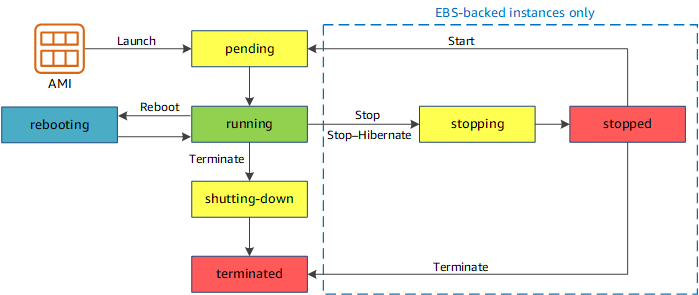
\includegraphics[width=0.8\textwidth]{figures/ec2_instance_lifecycle.png}
      \caption{Illustration of the state transitions of an EC2 instance~\cite{noauthor_instance_nodate}.}
      \label{fig:ec2_lifecycle}
  \end{center}
\end{figure}

\paragraph{Networking.} The instance is given a private and a public IPv4 address, where the private address is not reachable over the Internet but can be used for communication between endpoints within the same Virtual Private Cloud (VPC)\footnote{Amazon VPC builds a virtual network environment that users can control at will.}, while the public address is reachable over the Internet. The private IPv4 remains associated with the network interface during the lifecycle, while a public IPv4 is reassigned each time the instance transitions to the running state. Security groups\footnote{Security groups allow users to control traffic and act as a custom virtual firewall.} can be used to configure a virtual firewall and restrict incoming and outgoing traffic based on type, protocol, port, and source.

\paragraph{Pricing.} The lifecycle shown is important later when our orchestrator manages the EC2 instance, but the lifecycle also plays a crucial role in understanding the EC2 billing process. Once an instance enters the running state, it will be charged for every second it keeps running, with a minimum of one minute. The price depends heavily on the instance type, the price for the \code{t2.micro} instance is \$0.0134 per hour. There are several ways to pay for EC2 instances: On-Demand, Savings Plans, and Spot Instances. Everything covered in this section refers to on-demand instances as we have used them. Savings plans reduce the price in exchange for a consistent amount of usage commitment. In contrast, Spot instances allow one to request free EC2 capacity at reduced prices, suitable for stateless, fault-tolerant, or flexible applications~\cite{noauthor_secure_nodate}.

\subsubsection{Application in Practice: Self-Hosted Redis}
The EC2 computing platform can be used to host a wide range of applications. The platform also offers the option of setting up a self-hosted Redis cluster. We use the term ``self-hosted'', even though the servers are deployed in the cloud, to illustrate the difference from the fully managed Amazon ElastiCache for Redis service in the next section. Getting a self-hosted Redis server up and running is relatively easy, while the real work is to monitor, maintain and properly configure it to meet requirements. Redis can be downloaded to an EC2 instance and set up as a daemon that runs when the EC2 instance enters the running state. When setting up a Redis cluster on multiple machines with sharding and multiple read replicas, the process to get each node up and running is similar. For the system administrator, the more challenging part is setting up each node configuration correctly to get the desired cluster.

~\\
Once the self-hosted Redis server or cluster is correctly configured, the system administrator is still responsible for keeping the instance only running if the cache is actually needed to avoid unnecessary costs. The system administrator is also responsible for scaling and maintaining the whole system. This entire process can be done manually or through automation. Later, we use the term ``automation process'' to describe the effort required for the system administrator to maintain and manage the self-hosted Redis server or cluster in a cost-effective manner using automation scripts. 

% Once the self-hosted Redis server or cluster is up and running, the system administrator is still responsible for scaling and maintaining the system. This entire process can be done manually or through automation. Automation requires querying the system for certain metrics and triggering scaling based on the metrics received. While there are some third-party tools available to assist the system administrator, it is still a significant amount of work to get everything up and running as intended.

% ElastiCache or Self-Hosted Redis on EC2: Which is the One For You?~\cite{noauthor_elasticache_nodate}.

\subsection{ElastiCache}
\label{subsec:elasticache}
Amazon ElastiCache is a Cache-as-a-Service on the AWS platform that uses either Redis or Memcached as its caching engine~\cite{noauthor_amazon_nodate-1}. The caching layer provided by ElastiCache is the same as self-hosted Redis, except that it is a fully managed service that takes care of provisioning, monitoring, and updating. More specifically, ElastiCache allows setting up Redis in a few clicks without ever touching the actual server(s). When creating an ElastiCache Cluster, one can enable or disable cluster mode and specify the number of replicas. If cluster mode is enabled, the number of shards can be specified, and the number of replicas is then considered the number per shard. The actual memory capacity is selected per node by specifying the desired node type, similar to the instance types for EC2. A few AWS-specific settings remain, but at this point, one is ready to confirm the creation of the ElastiCache cluster. Once up and running, the Redis cluster is configured, running, and seamlessly maintained without worrying about it. \emph{Performance at Scale with Amazon ElastiCache}~\cite{noauthor_performance_nodate} provides a good overview as well as the official documentation~\cite{noauthor_comparing_nodate}.

\paragraph{Cluster Mode Disabled vs. Enabled.}
% cluster mode enables vs disabled
Deploying a Redis cluster in disabled cluster mode is similar to Redis Sentinel, where the cluster is built from a single shard. Therefore, the only way to scale for more memory and better write throughput is to scale the node type. For read scaling, one can have up to five read replica nodes. In enabled cluster mode, vertical scaling is still possible, but sharding allows to scale the number of shards in addition to the number of replicas per shard. ElastiCache allows users to scale the node type or cluster configuration with a few clicks or through the AWS command-line interface without worrying about the underlying process of provisioning new instances or copying the data to the new node type.

\paragraph{Auto Scaling.}
% only available for cluster mode enabled
% https://docs.aws.amazon.com/AmazonElastiCache/latest/red-ug/Replication.Redis-RedisCluster.html
In August 2021, Amazon added a new feature to ElastiCache, Auto Scaling. Using AWS Application Auto Scaling and CloudWatch metrics, ElastiCache provides the ability to set automatic scaling policies. ElastiCache for Redis then automatically scales according to the policies by either adding/removing shards to the cluster or adding/removing read replicas, similar to the manual scaling described above. ElastiCache auto-scaling enables two types of scaling policies:
\begin{itemize}
  \item Target tracking scaling policies adjust resources based on a target value for a specific metric (e.g., memory usage).
  \item Scheduled scaling policy: Create scheduled actions to scale at specific times to handle predictable load changes.
\end{itemize}
It is important to note that auto-scaling is only available for ElastiCache in enabled cluster mode and that there are additional restrictions on ElastiCache node types. Only instance type families \code{R5, R6g, M5, M6g} and instance sizes \code{Large, XLarge and 2XLarge} are supported.

~\\
Scaling is possible both online and offline; although performance is affected by the computationally intensive scaling operations when scaling online, the server continues to process requests during the scaling process. The scaling process takes time, as it may require copying the entire database to a new node or online resharding, which involves rebalancing the shards. Thus, ElastiCache Auto Scaling ensures that a scaling action is not triggered lightly by monitoring whether the target value exceeds the specified metric over an extended period of several minutes~\cite{noauthor_auto_nodate}.

\paragraph{Pricing.} Billing is similar to EC2; there are on-demand and reserved nodes, with a discount offered for long-term commitments. The price is tied to the instance type used and is billed hourly instead of seconds for EC2. Node type names include a cache before their name, while naming conventions are the same as EC2 instances. The price per hour for \code{cache.t2.micro} is \$0.019. A portion of the memory is used for system overhead for each node. So while the EC2 node type \code{t2.micro} provides 1 GiB of memory, the corresponding ElastiCache node type \code{cache.t2.micro} provides only 0.555 GiB of memory. For the next larger node type \code{t2.small} with 2 GiB of memory, the corresponding ElastiCache node type provides 1.55 GiB of memory.

% ElastiCache or Self-Hosted Redis on EC2: Which is the One For You?~\cite{noauthor_elasticache_nodate}.
% Performance at Scale with Amazon ElastiCache~\cite{noauthor_performance_nodate}.

\subsection{Serverless Computing}
\label{subsec:lambda}
In general, Cloud computing or Infrastructure-as-a-Service (IaaS) is widespread and popular in practice. The pay-as-you-go model and the ability to scale without investing in hardware allowed cloud providers to take over a large portion of IT organizations' annual software and IT infrastructure spending. This clearly shows how popular cloud-based services like EC2 are. If resources are used as efficiently as possible, there is little for users to complain about. However, the responsibility for scaling lies with users, often leading to over-provisioning to accommodate sudden increases~\cite{castro_rise_2019}. While cloud providers are trying to ameliorate this problem by providing additional services such as EC2 Auto Scaling to help users use resources as efficiently as possible, cloud providers have also released a new approach to this problem, called serverless computing. 

~\\
Serverless computing is a computing platform like EC2 where servers are hidden from developers and code is run on demand and charged for actual execution time. Serverless computing is often referred to as Function-as-a-Service (FaaS). It allows developers to focus on implementation rather than the actual provisioning, resource allocation, and auto-scaling that is now handled by the cloud provider~\cite{eismann_serverless_2021}. The stateless nature of serverless computing is a challenge for applications that rely on state sharing or require data exchange~\cite{jonas_cloud_2019, klimovic_pocket_nodate}. Popular use cases are currently tightly coupled to the provided features of serverless computing, i.e., mainly event-driven workloads that can leverage the ability to scale from zero to infinity~\cite{jonas_cloud_2019}. However, it is important to note that serverless computing has attracted the attention of industry and academia and is constantly evolving to overcome particular challenges, making it a potentially leading platform in the future. Much work is done in benchmarking or architecture analysis~\cite{wang_peeking_2018, scheuner_function-as--service_2020}. There are also attempts to improve or extend the current architecture based on their needs~\cite{shahrad_serverless_2020, wawrzoniak_boxer_2021, wang_galleon_2021}. Others seek to solve challenges in the current paradigm of serverless computing~\cite{moyer_punching_2021, klimovic_pocket_nodate}. Exploring the possibilities of the serverless computing paradigm is of general interest and has led to several interesting projects that include serverless computing as a building block~\cite{wang_infinicache_2020, mahgoub_sonic_2021, thomas_particle_2020, noauthor_granular_nodate}.

~\\
In our work, we focus on AWS Lambda, Amazon's serverless computing service~\cite{noauthor_serverless_nodate}. We explore the capabilities of the serverless platform to provide in-memory caching capabilities. When creating a AWS Lambda function, the platform packages the function code into a container that runs on the multi-tenant cluster of machines managed by AWS. The user only has to specify the function code and some parameters about the function (runtime, architecture, memory, timeout), while the CPU is allocated proportionally to the amount of memory. Invoking a function is event-based, AWS supports several possible events: HTTP requests via Amazon API Gateway\footnote{Fully managed service for APIs.}, object changes on S3, table updates in Amazon DynamoDB\footnote{Fully managed, key-value NoSQL database.}~\cite{noauthor_fast_nodate}, or simply via the Invoke API provided by their SDK. The Invoke API supports synchronous (wait for response) and asynchronous calls. 

\begin{figure}[ht!]
  \begin{center}
      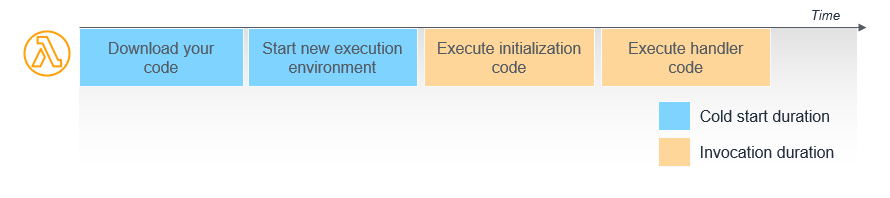
\includegraphics[width=0.8\textwidth]{figures/lambda_invoke.png}
      \caption{Illustrates the process of setting up an execution environment for AWS Lambda and then running the function code~\cite{noauthor_operating_2021}.}
      \label{fig:lambda_invoke}
  \end{center}
\end{figure}

\paragraph{Execution Environment.} Once the function is invoked, an execution environment on a Lambda Worker is created or assigned if a matching one already exists. Each execution environment may be used for only one concurrent invocation, while many instances of the same function can be executed concurrently. AWS Lambda continuously monitors and manages the execution environments, creating new environments and destroying old ones. Creating an execution environment includes downloading the code for the function and setting up the environment with the memory, runtime, and configuration as specified by the user. Once the environment setup is complete, Lambda executes the initialization code before executing the actual handler code, as shown in Figure~\ref{fig:lambda_invoke}. The first two steps are also referred to as a \emph{cold start}, which adds latency to the invocation process but is not charged for. After the function returns, Lambda keeps the execution environment for a non-deterministic period of time to optimize resource management and performance. Thus, if a new request for the same function arrives on time, the execution environment can be reused, resulting in a faster startup time, called a \emph{warm start}~\cite{noauthor_security_nodate, noauthor_operating_2021}.

\paragraph{Reusable Execution Environments.} The cold start concept compared to warm start has some additional effects despite the shortened start time. Reusing the execution environment also means that local state and even outgoing connections remain available. This can be used to save costs by reducing the actual execution time, as stated in the official documentation, but also provides many opportunities to use the serverless platform as a pay-as-you-go storage~\cite{wang_infinicache_2020}, which may not have been their intention. The duration that the execution environment remains is not deterministic, making it challenging to use this mechanism reliably. For security and data leakage reasons, care should be taken when using the execution environment to store data across invocations.

\paragraph{Networking.} Lambda function in a VPC does not have access to the Internet but can connect to other services in the same VPC. The significant problem is that AWS Lambda blocks inbound network connections but supports outbound TCP/UDP connections. NAT traversal techniques can be used to work around this limitation, for example, to allow direct communication between serverless functions~\cite{moyer_punching_2021}. 

\paragraph{Pricing.} Billing is based on the number of requests to the function and the function execution duration. The duration includes only the time when the actual function code (initialization code and handler code) was executed. Billing granularity is much finer on a millisecond basis compared to EC2. The price per millisecond depends on the amount of memory specified by the user. The minimum amount of memory is 128 MB and costs \$0.0000000021 per 1ms, 1024 MB costs \$0.0000000167, while the maximum amount is 10240 MB for \$0.0000001667 per 1ms. The price per millisecond is linearly proportional to the amount of memory available and thus to the CPU capacity.

\chapter{Design}
\label{cha:design}
In this chapter, we motivate the design of a reactive caching system with serverless computing in Section~\ref{sec:system_goals}. In Section~\ref{sec:system_overview}, we give a general overview of our system and its building blocks, while Section~\ref{sec:system_workflow} introduces the system workflow and how those building blocks interact with each other. Chapter~\ref{cha:implementation} describes the implementation of the individual blocks in more detail.


\section{Design Goals}
\label{sec:system_goals}
Modern applications often rely on in-memory caching to improve latency-sensitive parts of their applications. Read-intensive applications can benefit significantly from in-memory caching by avoiding repeated accesses to the slow database or repeated, expensive queries of the database. Multiple distributed in-memory key-value stores, such as Memcached and Redis, are already available to provide optimized performance. In-memory caching is more expensive than slower tiers such as hard disks or SSDs, but it offers a huge performance boost, which is the main incentive for using in-memory caching. 

~\\
We first take a brief detour to Redis-based systems, which form the foundation of our in-memory caching layer and compare self-hosted Redis with ElastiCache for Redis to understand the need for a reactive in-memory caching system. We point out the current elasticity limitations regarding a fully managed service and mention the challenges of cost-effective maintenance of self-hosted Redis. This leads to the problem setting we focus on in this work and helps understand the reactive design of our system described at the end. 

\subsection{Redis-based Caching}
ElastiCache for Redis offers caching as a service within a few clicks without bothering about the actual servers underneath. The running Redis cluster is conceptually the same as a self-hosted Redis cluster on EC2 instances. However, everything ElastiCache offers is done in a few clicks, whereas with self-hosted Redis, the system administrator has to take care of it (without a simplified web interface). We mentioned an automation process that the sysadmins could use to avoid having to do this manually, but this requires a lot of effort to set up the automation process in the desired way and burdens him with much responsibility. Auto-scaling is an additional feature for ElastiCache that allows the cluster to scale as needed. The same behavior can be achieved with the automation process, only with more effort than a few clicks. Of course, the managed service comes at a price, so when comparing the hourly price, it is not surprising that the ElastiCache instance (\code{cache.t2.micro}) costs \$0.019, while the EC2 instance (\code{t2.micro}) costs \$0.0134. When comparing larger node type families, the factor even increases according to the prices on the official documentation. Another big difference is the billing granularity. While EC2 is billed per second with a minimum billing granularity of 60 seconds, ElastiCache uses a billing granularity of one hour. So as long as the cost is not an issue, ElastiCache provides a service that requires minimal system administrator effort to maintain a running and easily scalable Redis cluster. However, if cost reduction is the primary concern and the associated sysadmin effort does not get in the way, self-hosted Redis offers more customization options and finer-grained control over the Redis cluster. 

~\\
Thus, the pay-per-use model of ElastiCache is based on node hours compared to node seconds for self-hosted Redis on EC2. Depending on the billing granularity, the cost-effectiveness of the fully managed system depends heavily on the actual workload. So imagine a workload with a certain base utility and a short burst workload at the beginning of each hour that triggers ElastiCache's auto-scaling to provision an additional node for a full hour. In addition, ElastiCache is not designed for situational usage, as a cluster cannot be stopped to prevent billing if it remains unused but can only be deleted and recreated. This, combined with the billing granularity, significantly limits the cost-effective elasticity of ElastiCache for these specific workloads. 

~\\ 
On the other hand, Self-Hosted Redis is also not cost-effective in the case of burst workloads if the instance is running for the entire hour. With self-hosted Redis, the system administrator can dynamically start and stop the Redis instance to avoid paying for unused time. However, there is still some start-up time required before Redis is available. Therefore, it is difficult to set up an automation process for self-hosted Redis for burst workloads with unknown arrival times. The sysadmin either risk preemptively starting the in-memory caching layer without using it, which adds unnecessary cost, or reacting to the load, which results in poor performance because it takes time for the EC2 instance hosting the Redis server to become available. So building a cost-effective in-memory caching system in this scenario is difficult if one does not know the workload in advance. 


\subsection{Problem Setting}
The mentioned burst workloads are the primary problem setting within the scope of this work. Burst workload means only the time duration for which in-memory caching is required. For example, a burst workload of five minutes means that in-memory caching is only required for the duration of that burst, i.e., five minutes, while the rest of the time, the cache runs without being used. In the context of this work, we focus on the case where a single Redis instance can handle a load of such a burst for simplicity. The previous section has shown why providing in-memory caching for such bursty workloads can be difficult or cost-inefficient with a pure Redis-based system.

\subsection{Reactive Caching}
We address the above problems by building a reactive in-memory caching system in this work. Table~\ref{tab:layers} provides an overview of the different memory layers used in our system and their key characteristics. While self-hosted Redis is the foundation of our in-memory caching system, the main contribution of our work is the reactive design to build a cost-effective in-memory caching system and the integration of an additional in-memory caching layer in the form of serverless computing. The reactive design avoids over-provisioning of in-memory caching resources and therefore enables a cost-effective system. We emphasize the importance of responsiveness when building an in-memory caching system, as a reactive system based only on self-hosted Redis that takes a few dozen seconds to provision in-memory caching capacity is clearly suboptimal. To mitigate the long startup times of EC2 instances for self-hosted Redis, which are on the order of 30 seconds, serverless compute units are less cost-effective but available within milliseconds. The reactive design of our in-memory caching system can respond within milliseconds by leveraging the serverless platform and transitioning to the lower-cost, self-hosted Redis layer if the load persists.

\begin{table*}[t]
    \centering
    \ra{1.2}
        \begin{tabular}{ @{}l l l l l l@{} }
        \toprule
          & Layer & Latency & Startup Time & Cost & Pricing-Model \\
        \midrule
        S3 & Storage & High & - & \$ & request \& storage cost \\
        Lambda & Cache & Low & $\sim$20ms (warm-start) & \$\$\$ & billed per ms \\
         & & & $\sim$500-700ms (cold-start) & & \\
        Redis & Cache & Low & $\sim$20-50s & \$\$ & billed per second \\
        \bottomrule
        \end{tabular}
    \caption{This table shows the key characteristics of the different layers in our system. S3 is the persistent storage backend, while the in-memory caching layer includes self-hosted Redis and serverless computing.}
    \label{tab:layers}
\end{table*}

~\\
In the context of this work, we focus on the scenario of burst workloads durations less than an hour for fixed-size in-memory caching. The evaluation in Chapter~\ref{cha:evaluation} provides more details about the workload characteristics to motivate our approach, while Chapter~\ref{cha:discussion_and_outlook} discusses future work to extend our system to a fully managed scalable in-memory service similar to ElastiCache.

% Our system attempts to solve this problem by providing an additional layer of in-memory caching in the form of serverless compute units that benefit from startup times in the order of milliseconds, compared to startup times of around 30 seconds when using self-hosted Redis on EC2 instances. The additional layer is used to build a reactive system that is able to respond in time, and for the transition period where we set up a Redis cache in case the load persists. 

% \subsection{Why not just use ElastiCache?}
% % \paragraph{Amazon ElastiCache for Redis vs. Self-Hosted Redis on EC2}
% % specify differences and specifc use cases
% Building a Redis-based managed caching system raises the question of why not just use ElastiCache. This section clarifies the difference of self-hosted Redis and ElastiCache and motivates the design of our reactive caching system compared to ElastiCache.

% ~\\
% ElastiCache for Redis offers caching as a service within a few clicks without bothering about the actual servers underneath. The running Redis cluster is conceptually the same as a self-hosted Redis cluster on EC2 instances. However, everything ElastiCache offers is done in a few clicks, whereas with self-hosted Redis, the system administrator has to take care of it. We mentioned an automation process that the sysadmin can use to avoid having to do this manually, but this requires a lot of effort to set up the automation process in the desired way and burdens him with a lot of responsibility. Auto-scaling is an additional feature for ElastiCache that allows the cluster to scale as needed. The same behavior can be achieved with the automation process, only with more effort than a few clicks. Of course, the managed service comes at a price, so when comparing the hourly price, it is not surprising that the \code{cache.t2.micro} ElastiCache instance costs \$0.019, while the \code{t2.micro} EC2 instance costs \$0.0134. When comparing larger node type families, the factor even increases. Another big difference is the billing granularity. While EC2 is billed per second with a minimum billing granularity of 60 seconds, ElastiCache uses a billing granularity of one hour. So as long as cost is not an issue, ElastiCache provides a service that requires minimal system administrator effort to maintain a running and easily scalable Redis cluster. However, if cost reduction is the primary concern and the associated sysadmin effort does not get in the way, self-hosted Redis offers more customization options and finer-grained control over the Redis cluster. 

% ~\\
% Situational use of ElastiCache is difficult because the cluster cannot be stopped, only deleted and recreated. So ElastiCache doesn't really provide scaling to zero, and even if delete and recreate does the trick, ElastiCache's billing granularity still strongly discourages its use as a cost-effective situationally used cache. Self-hosted Redis, on the other hand, is a suitable building block in building a reactive in-memory caching service using serverless computing. The evaluation and discussion will further address this topic.


% This section compares the managed service ElastiCache to self-hosted Redis and explains the reference to our work. ElastiCache manages the whole server hosting and managing/monitoring which results in an easy setup within a few clicks but less flexibility with respect to the cluster configuration. Scaling takes much less effort with ElastiCache and even supports setting up auto-scaling with a few clicks, whereas with self-hosted Redis, the system administrator has to do this either manually by setting up new instances or through automation scripts, which puts a lot of responsibility and effort on the system administrator~\cite{noauthor_elasticache_nodate}. 

% When comparing prices, we consider the same node type and assume that the system overhead for the self-hosted Redis is about the same. The ElastiCache node type price for \code{cache.t2.micro} is \$0.019 per hour, while the EC2 price is \$0.0134. Without much surprise, the managed service is more expensive with a factor of 1.418. The factor for the \code{cache.r5.large} node type is 1.71 and for the \code{cache.m6g.large} node type even 1.92. Remember that Redis is mostly single-threaded (I/O handler), so using instances with multiple vCPUs does not directly increase performance as stated in the AWS documentation: you need to multiply the reported CPU usage by the number of CPU cores to get the actual usage of the single core that Redis uses~\cite{noauthor_performance_nodate}. In comparison, self-hosted Redis can easily use multiple CPUs by launching multiple instances on the same server, thus building a multi-tenant system that uses all available CPU capacity.


\section{Design Overview}
\label{sec:system_overview}
% Our system consists of several building blocks: a single orchestrator, a reverse proxy, a storage backend, and the in-memory caching layer.
This section provides a general overview of our system and its building blocks, as shown in Figure~\ref{fig:system_overview}. Clients interact with the reverse proxy to retrieve the value of a particular key. The reverse proxy acts only as a gateway, forwarding the request to the appropriate endpoint and sending back the associated response. The orchestrator manages the entire system, including the caching layer, and provides the reverse proxy with the necessary information about the corresponding endpoint. The storage backend stores key-value pairs in persistent storage, while the caching layer is responsible for high-frequency reads and consistent throughput through in-memory caching. Our in-memory caching layer consists of two building blocks based on AWS Lambda's serverless platform and the other on self-hosted Redis with EC2 instances. Although both provide in-memory capacity, the actual use case is very different due to their characteristics, as described in the previous section. The endpoint used by the reverse proxy is either the backend storage in the form of S3 or the caching layer that the orchestrator occasionally sets up. When and how our orchestrator decides to deploy an in-memory caching layer is resolved by an event-based reactive scheduler, where events contain information about recent requests in the past provided by the reverse proxy.

\begin{figure}[ht!]
    \begin{center}
        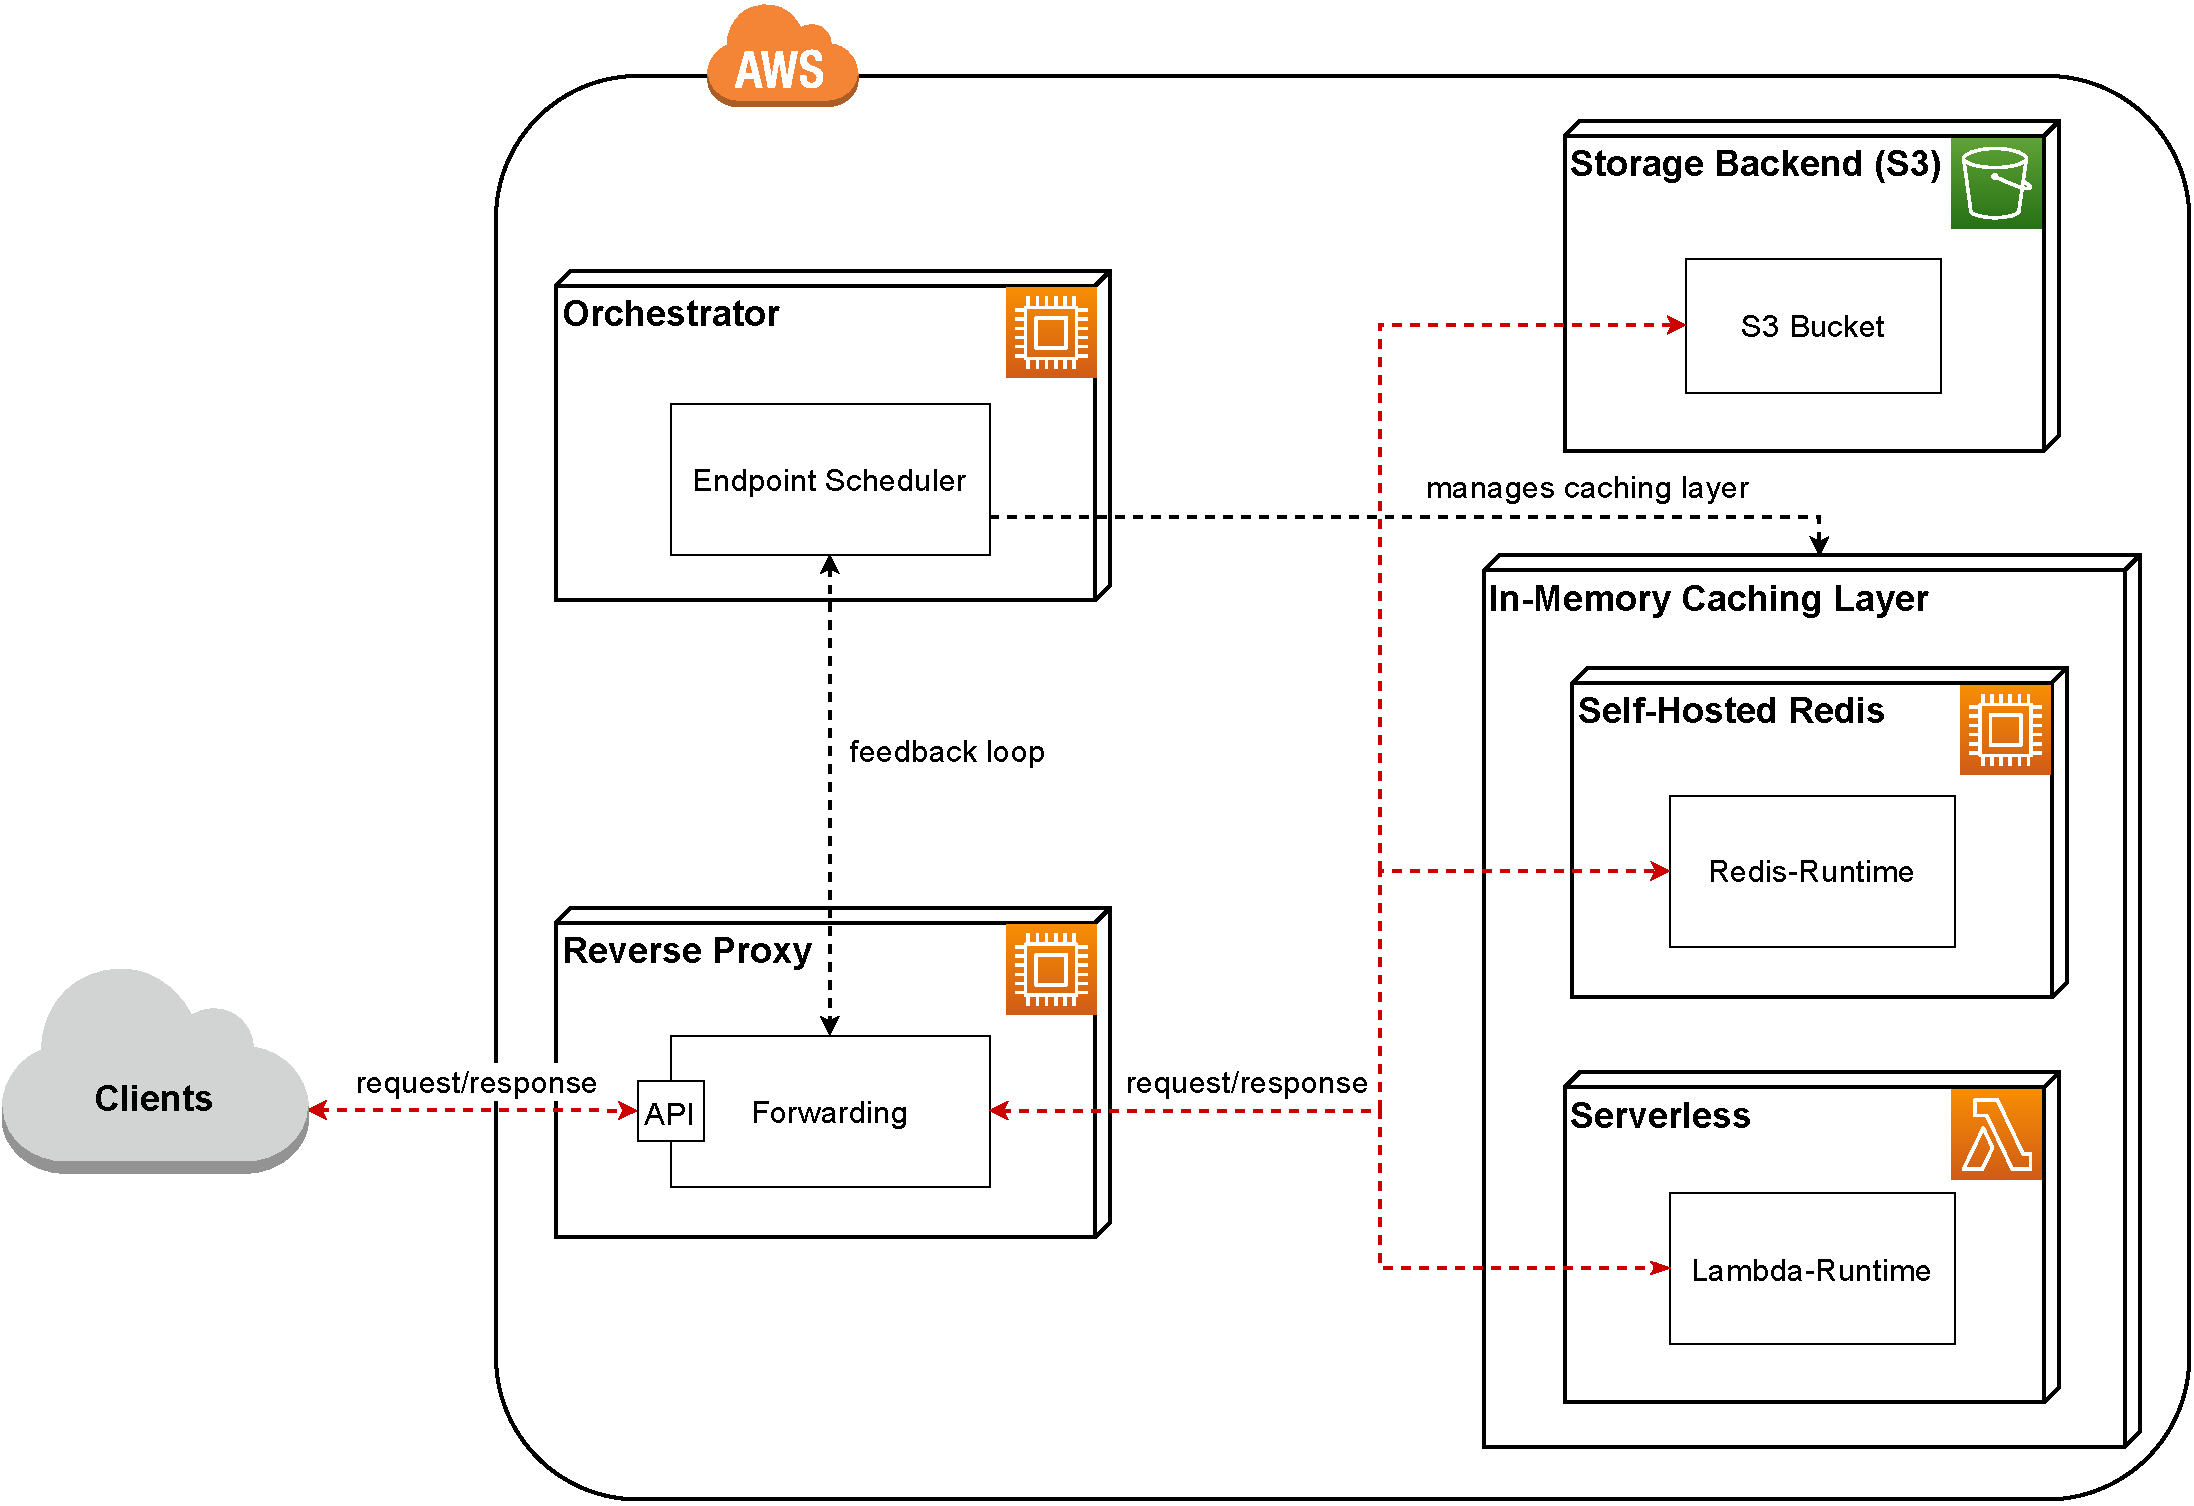
\includegraphics[width=0.95\textwidth]{figures/system_overview.pdf}
        \caption{General overview of the building blocks of our system. Only the main communication is shown, while a more detailed communication overview is given below for each individual part.}
        \label{fig:system_overview}
    \end{center}
\end{figure}

~\\
Figure~\ref{fig:system_overview} only provides a general overview of our system and the main communication channels. In Chapter~\ref{cha:implementation}, each part of the system is discussed in more detail in terms of implementation and design decisions to solve the given challenges. We also focus on how each part interacts with the others and the communication required. By deploying the orchestrator on a separate EC2 instance, we have created a system that closely adheres to the primary/secondary communication model. Therefore, our orchestrator takes on the role of the primary node that controls the other parts of the system (secondary nodes). With this design pattern, we were able to build the system in a modular fashion while maintaining a high degree of flexibility in adapting parts to changing requirements. The last point is crucial as the requirements changed and also crucial in view of Chapter~\ref{cha:discussion_and_outlook}, where we will talk about future work and the way of integrating the necessary changes into our system.

\section{System Workflow}
\label{sec:system_workflow}
This section should help to understand the workflow of our system. We describe this from the perspective of a request arriving from the client, which is the most crucial functionality since our system is built as an in-memory caching system. Also, the main contribution of our work is based on the arrival of these requests since the orchestrator that manages the whole system is a reactive event-based mechanism. This provides a good overview for the next chapter, where we describe each building block in more detail with respect to the actual implementation.

~\\
The reverse proxy does exactly what its name suggests: It accepts requests from the client and forwards the request either to the memory backend or to a running in-memory caching layer. The storage backend and self-hosted Redis are simple in that they only act as a server, while a serverless function is not intended to act as a server to which requests can be forwarded. Section~\ref{sec:serverless} will cover the serverless platform in more detail. The memory backend is always available and therefore forms the default endpoint to which our reverse proxy forwards requests, while the in-memory caching layer only runs situationally. This leads to our orchestrator, responsible for managing the in-memory caching layer and thus forms the core of our system. The reverse proxy informs the orchestrator about the requests received, which form the events that our event-based reactive orchestrator works with. Our orchestrator responds quickly and uses the serverless platform to make in-memory caching available based on these events. If the load persists with respect to these events, the orchestrator uses the serverless platform until it successfully launches the self-hosted Redis instance. Therefore, the orchestrator is also responsible for keeping the reverse proxy endpoints up to date with respect to the managed in-memory caching layers. Thus, when a new request arrives at the reverse proxy, the request is forwarded to the in-memory caching layer and not to the storage backend. 

\paragraph{Endpoint Scheduler.}
We mentioned our orchestrator's event-based, reactive design, which we will refer to as our orchestrator's endpoint scheduler. The endpoint scheduler keeps a state for each object and follows a state diagram to manage the in-memory caching layers. The endpoint scheduler changes its state and thus provides in-memory caching to the reverse proxy based on the state and events. The state diagram models the endpoint that the reverse proxy should use. The way we use serverless computing as an additional in-memory caching layer forms the first layer that provides in-memory caching. This allows our reactive endpoint scheduler to quickly respond to events that indicate a need for in-memory caching. If the demand persists, the endpoint scheduler switches to self-hosted Redis and uses the serverless platform for the startup time required by the EC2 instance hosting Redis. The instance can also be shut down again by the endpoint scheduler, and we basically start over. 

\chapter{Implementation}
\label{cha:implementation}
Chapter~\ref{cha:design} gives a rough overview of what the individual building blocks in our system are responsible for and how the system is structured as a whole. In this chapter, we take a closer look at the individual parts and how they are implemented to provide the necessary functionality. While we go into more detail about the implementation of our system, we also mention some of the challenges we encountered while developing our system and how we overcame them. 

~\\
In Section~\ref{sec:reverse_proxy} we introduce the reverse proxy, its forwarding mechanics, and the messages that update these endpoints. 
The orchestrator contains the tools to manage the caching layers. Section~\ref{sec:orchestrator} describes those tools and introduces the endpoint scheduler, which uses these tools in the form of an event-based reactive mechanism, and is thus responsible for decision-making and setting up the caching layer. The storage backend and caching layer are also briefly covered; since S3 (see Section~\ref{sec:storage_backend}) and Redis (see Section~\ref{sec:self_hosted_redis}) do not require implementation, the focus is on the Lambda runtime (see Section~\ref{sec:serverless}). We explain how we leverage the serverless platform to create a server-like function that serves requests while AWS Lambda blocks incoming TCP connections. 

~\\
We chose Go as the implementation language for our system (orchestrator, reverse proxy, and Lambda runtime). Go is often used for cloud-based or server-side applications due to its high performance and built-in concurrency. The Go package \code{Redeo}~\cite{noauthor_redeo_nodate-1} was used to create Redis protocol-compatible TCP servers/services similar to InfiniCache~\cite{wang_infinicache_2020}.

\section{Reverse Proxy}
\label{sec:reverse_proxy}
The reverse proxy is the entry point for clients to retrieve key-value pairs by providing an API. Depending on the forwarding rules set by the orchestrator, the reverse proxy interacts with either the storage backend or the in-memory caching layer in the form of the Lambda runtime or self-hosted Redis. For the purposes of this work, we assume that the client is outside the AWS infrastructure without worrying about the actual client.

~\\ 
First, the reverse proxy implementation details are described in terms of startup and initialization. Then, the overall forwarding mechanic of the reverse proxy for API requests and how our system updates the endpoints are explained in more detail. 

\subsection{Startup}
At startup, the reverse proxy establishes a persistent TCP connection with the orchestrator, which is later used for client/server communication, with the reverse proxy acting as the client. The corresponding address of the EC2 instance running the orchestrator is determined using the AWS SDK and the hard-coded instance ID. The reverse proxy also starts two servers at startup, one for the orchestrator and the other for communication with the Lambda runtime. This way, we can provide a bidirectional client/server communication between the reverse proxy and the orchestrator. In order for the orchestrator and later the Lambda runtime environment to connect to the corresponding reverse proxy server, the reverse proxy sends a \emph{ProxyHello} message to the orchestrator after the connection is successfully established, which contains the required information about both server endpoints. Last but also most important, the reverse proxy launches an API with a corresponding \code{get} endpoint through which the client can request key-value pairs. The API is implemented with the Gin Web Framework\footnote{Uses the Go package \code{HttpRouter}~\cite{schmidt_httprouter_2022} compared to the Go standard package \code{net/http} for a powerful HTTP request router for better performance according to their documentation.}~\cite{noauthor_gin_2022}.

\subsection{Forwarding}
\label{subsec:forwarding}
The API endpoint for \code{get} requests on our reverse proxy must distinguish whether the requests need to be forwarded to backend storage or whether in-memory caching is available. In this section, we first describe how this forwarding process is implemented in more detail. We then address the challenge of forwarding requests to dynamic endpoints that can shut down at any time, called in-flight handling. Finally, we briefly discuss the messages that the reverse proxy receives responsible for keeping the endpoints up to date; when and which building blocks trigger these messages is described in their respective sections.

~\\
The reverse proxy uses a mapping for each key that is overwritten when changes are received for routing. As we will see later, multiple goroutines could read and overwrite these entries, so a safe mapping for concurrent use from the Go package \code{sync.map} is used. Controlled by this mapping, either S3, the running Lambda runtime, or the self-hosted Redis instance is queried. Before the request is forwarded, a goroutine sends a message to the orchestrator containing the key, the endpoint to use, and a Unix timestamp.

~\\
So far, we have only mentioned that the request is forwarded. We describe the implementation details depending on the endpoint in this section. For the backend storage and the self-hosted Redis, the process is basically the same, while for the Lambda runtime, we have to consider that the connection is not a traditional client/server connection. Accessing the storage backend is relatively self-evident with the \code{aws-sdk-go} for the S3 service. The value is downloaded and copied into the response and returned to the client. The package go-redis~\cite{noauthor_redis_nodate-1} is used to query the self-hosted Redis instance. The client is initialized with an address and password before the request arrives and then used to forward the request by using the \code{get} operation for the client. Section~\ref{subsec:lambda} explains connection management for the Lambda runtime in more detail and why we are not able to get the appropriate response to a request as in traditional client/server scenarios. While sending the request using the Lambda runtime client is straightforward, we have to make some additional preparations to receive the response. In addition to the key, we also send a universally unique identifier (UUID) in our \code{get} request. A go channel is created through which the response is forwarded by the goroutine handling the response. We store the channel in a mapping and use the UUID as the key to associate the response with the corresponding request. The response contains the UUID of the request so that the response handler can find the correct channel to forward the response to. Once we receive the response on the channel, it can be sent back to the client.

\subsubsection{In-Flight Handling} 
To prevent the case where our reverse proxy forwards a request to the caching layer while the corresponding layer is simultaneously shut down, we use two Reader/Writer mutual exclusion locks (\code{sync.RWMutex}). One for the self-hosted Redis and one for the Lambda runtime. Each time a request is forwarded, the goroutine handling the request claims the corresponding Read lock and releases the lock after the request is resolved. As long as a request for one of the caching layers is in-flight, claiming the Write lock will block. Both caching layers send a message to the reverse proxy before they shut down, asking the reverse proxy to acknowledge the message. So before we acknowledge such a message, the reverse proxy claims the Write lock, which is blocked as long as a request is in-flight. As soon as we claim it, we can safely confirm the shutdown. Updating the mapping beforehand prevents new requests from being in-flight for the given endpoint, so the caching layer can be safely turned off.

\subsubsection{Updates} 
Later in Section~\ref{sec:orchestrator}, we will see how the orchestrator makes decisions about the caching layer and how the two layers are started and handled. For now, we will focus only on the messages received by the reverse proxy and the resulting actions. The orchestrator receives the following messages:
\begin{itemize}
    \item \emph{RedisStart}: Contains the address of the self-hosted Redis instance used to initialize a new Redis client.
    \item \emph{RedisUpdate}: Informs the reverse proxy about added or removed keys in the Redis instance. Adding sets the corresponding mapping entry to the Redis endpoint, while removing deletes the entry.
    \item \emph{RedisStop}: Claims the Write lock for Redis, removes the Redis client and sends an acknowledgment back.  
\end{itemize}
Similar to the orchestrator, the Lambda runtime also sends two messages to the reverse proxy:
\begin{itemize}
    \item \emph{LambdaStart}: Contains the key that is now served by the Lambda runtime and sets the corresponding mapping entry to the Lambda endpoint.
    \item \emph{LambdaBye}: The message contains the key of the Lambda runtime that is currently being shut down. Checks the mapping and deletes the entry if the current Lambda endpoint is included. Otherwise, no action is taken, indicating that a message from the orchestrator has already overwritten the entry. Unlike the Redis shutdown acknowledgment mechanism, the message handler starts a goroutine that claims the Lambda Write lock and sends a separate acknowledge message instead of a response. This is necessary because bidirectional client/server communication with the Lambda runtime is not possible due to the limitation of incoming connections.
\end{itemize}

\section{Orchestrator}
\label{sec:orchestrator}
% Object Manager
% Self-hosted Redis instance management.
% Lambda function invoke handling.
The reverse proxy is responsible for actually forwarding the client requests, while the orchestrator works in the background to ensure that the reverse proxy operates as intended and that the corresponding in-memory caching layer is managed as expected. 

~\\
First, we cover the startup and initialization of the orchestrator. We then present the tools and implementation details that the orchestrator needs to manage the in-memory caching layers in Section~\ref{subsec:orchestration_cachinglayer}. We cover how the orchestrator manages the EC2 lifecycle for the self-hosted Redis instance and how the serverless functions are invoked as an additional in-memory caching layer. Section~\ref{subsec:endpoint_scheduler} then explains the reactive design of our system by introducing the orchestrator's endpoint scheduler, which is responsible for managing the in-memory caching layers based on a state diagram. The endpoint scheduler is modeled as a reactive event-based mechanism that uses a feedback loop with the reverse proxy for events and keeps the endpoints on the reverse proxy up to date.

% Section~\ref{subsec:endpoint_scheduler} then explains reactive design of our system by covering the logic behind the orchestrator, which we call the endpoint scheduler. The state of the current implementation models our endpoint scheduler as a reactive, event-based mechanism where events are messages from the proxy that inform our orchestrator of the latest requests served. Choosing a simple and transparent mechanism as our endpoint scheduler helped get the system up and running quickly and provide insight into the capabilities of our system. 

\subsection{Startup}
The startup is similar to the reverse proxy by starting two servers, one for the communication with the Lambda runtime and the other for the reverse proxy. The server for the reverse proxy is required once the proxy is up and running. Recall that one of the first actions of the reverse proxy after establishing a connection to the orchestrator is to send a startup message containing the addresses of the two endpoint servers running on the reverse proxy. After receiving the message, the orchestrator also establishes a persistent TCP connection to the reverse proxy for client/server communication. This time the orchestrator acts as a client resulting in the bidirectional client/server communication channel. In addition, the orchestrator loads a system configuration file at startup, which is explained in more detail in Section~\ref{subsec:endpoint_scheduler}. It also initializes the \emph{RedisServerInstance} structure, which is used when interacting with the self-hosted Redis instance to keep track of the status of the EC2 instance running the Redis server, elaborated in more detail below.

\paragraph{Development API.} At startup, the orchestrator sets up a publicly available API that can be used to test and control the system. This is not used by the system but is worth mentioning because it was used extensively for testing before the system ran properly in its entirety. It contains endpoints for starting and shutting down the self-hosted Redis instance and interacting with it using standard Redis operations and the \code{ping} command. The API also includes endpoints to start and stop the Lambda runtime and an additional endpoint to log the current state of the reverse proxy forwarding rules on the console.  

\subsection{Orchestration of the Caching Layer}
\label{subsec:orchestration_cachinglayer}
This section covers the actions performed by the orchestrator to start, set up, and stop the caching layer components. This includes the required communication with other parts of the system. In the next section on the endpoint scheduler, we will see how these actions are actually applied in the running system. The role of the orchestrator for the self-hosted Redis part is much more extensive than simply invoking the serverless function that acts as Lambda runtime. Therefore, in this section, we only briefly cover the invocation process, while Section~\ref{sec:serverless} explains in more detail the design of our serverless function that acts as a caching layer component.

\subsubsection{Self-hosted Redis} 
As mentioned in Section~\ref{subsec:ec2}, our self-hosted Redis server runs on the EC2 compute platform as a daemon. As soon as the instance is up, the daemon starts, and the corresponding Redis server is available a short time later. The general role of the orchestrator is to start the instance as soon as the self-hosted Redis cache layer is requested and to shut it down if we decide otherwise. To track the status of the instance, the orchestrator maintains the \emph{RedisServerInstance} structure containing the instance ID, the address, and the status. At startup, the structure is initialized by querying the status of the EC2 instance using the AWS SDK for the EC2 service and the hard-coded instance ID. The address is set when the instance enters the running state and removed when stopped. We use two levels of abstraction in the implementation, where the first level is at the Redis level, and the underlying level is about the EC2 instance running the daemon. The Redis layer interacts with the EC2 instance layer to start and stop the instance as needed. This abstraction serves to separate the tasks of each layer clearly. The EC2 layer is responsible for managing the lifecycle transitions of the EC2 instance and informing the Redis layer of the transitions. While the Redis layer initiates these state transitions, it ensures that the actual Redis server daemon is up and running and notifies the reverse proxy about it. Due to the time required for the state transitions and the startup time of the daemon, we designed those two layers in a non-blocking manner by using goroutines and channels to notify each other.

~\\
Initially, the instance is in the stopped state, and when the orchestrator decides to start the Redis server, we initiate the startup at the Redis layer. A channel can be provided that is used as a signaling mechanism to notify the caller when the Redis server is ready. The Redis layer initiates the EC2 startup at the second layer and again uses a signaling channel to be notified when the instance enters the running state. We get the address of the running EC2 instance on this channel, which is used to create a new Redis client. Using the Redis client, we periodically \code{ping} the Redis server. When we get back a successful \code{pong}, we know that the Redis server is up and running and inform the reverse proxy with the \emph{RedisStart} message, which provides it with the required address to create a Redis client itself.

~\\
When the orchestrator requests to stop the Redis server, we query the list of current keys and inform the reverse proxy in the \emph{RedisUpdate} about the removed keys. Afterward, we send the message \emph{RedisStop} to the reverse proxy, which uses the acknowledgment mechanism described above for in-flight requests. So after we receive the acknowledgment, we can safely delete the Redis key-value pairs, remove the Redis client, and finally shut down the EC2 instance using the second layer. The caller can provide a channel to get notified as soon as the instance enters the stopped state.

~\\
In Section~\ref{subsec:ec2} we discussed that the instance is only billed when it is in the running state; this is important later for evaluating the cost of our system. When we ask the Redis server to start, the provided channel is notified when the instance enters the running state and starts accounting. For shutdown requests, billing ends when the function returns, while the channel is used to notify when the instance enters the stopped state, which means we can restart the instance.

\subsubsection{Lambda Runtime} 
Starting the Lambda runtime is simply a matter of invoking the Lambda function using the AWS SDK for the Lambda service. The function is called synchronously with the function name and a payload received from the handler code as function arguments. The payload includes the key of the key-value pair to be served by the Lambda runtime and a \emph{TICK} duration, the use of which is explained in Section~\ref{sec:serverless}. Also, the payload contains two addresses, one for the orchestrator server and the other for the reverse proxy server (which was received in the \emph{ProxyHello} message). Remember that this call blocks because of the synchronous requests. Once the Invoke returns, the Lambda runtime environment has either finished executing, crashed, or reached the timeout limit.

\subsection{Endpoint Scheduler}
\label{subsec:endpoint_scheduler}
% explain the general concept of the endpoint scheduler
% reactive, event-based mechanism
% events are
Our orchestrator now has all the tools to start and manage the in-memory caching layer. What is still missing is the reactive event-based mechanism, the endpoint scheduler. We mentioned the endpoint scheduler and the state diagram that models the endpoint used by the reverse proxy. The endpoint scheduler maintains a state for each object and follows the state diagram shown in Figure~\ref{fig:endpoint_scheduler}. Requests received by the reverse proxy are used as events that, together with the current state and additional parameters, trigger the transition within the state diagram and thus change the endpoint on the reverse proxy. 

~\\
First, we provide an overview of the state diagram and our endpoint scheduler and describe the system parameters used in the state diagram. We then explain in detail the implementation of our reactive event-based mechanism. Finally, we introduce the system configurator, which is used to derive the required system parameters for our system.

\begin{figure}[t]
    \begin{center}
        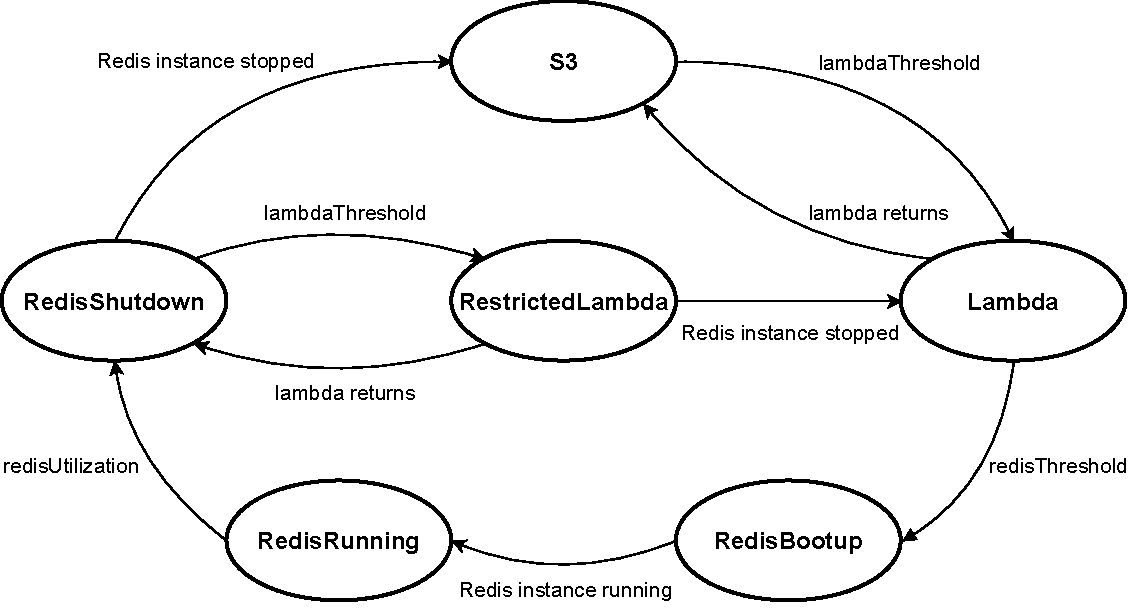
\includegraphics[width=0.8\textwidth]{figures/endpoint_scheduler.pdf}
        \caption{State diagram of the reactive, event-based endpoint scheduler.}
        \label{fig:endpoint_scheduler}
    \end{center}
\end{figure}

\subsubsection{State Diagram}
Initially, only the backend storage is available, which is referred to as state \textsc{S3}. We motivated serverless computing as a rapidly available additional in-memory caching layer. Thus, when our endpoint scheduler decides to provide in-memory caching, it switches to the \textsc{Lambda} state. This decision is based on a threshold for the number of requests received within a given time window. The following state transition is a bit more complicated due to the way we use the serverless platform, but simply put, the endpoint scheduler decides to either return to the \textsc{S3} state and turn off the serverless in-memory layer, or, if the load persists, use the less expensive self-hosted Redis layer. The time required to make the EC2 instance hosting Redis available is represented by the state \textsc{RedisBootup}. We continue to use the serverless platform for in-memory caching in this interim. Once the instance is up and running, the event-based design is suboptimal because we could get stuck in this state and the instance will be up and running forever. Therefore, to decide whether the endpoint scheduler should stop the Redis instance, a timer is used to re-evaluate the decision periodically. At this point, we cannot directly return to the \textsc{S3} state because the Redis instance is still shutting down, which prevents our system from restarting the instance immediately. To model this situation, we use the \textsc{RedisShutdown} state, which is basically the same as \textsc{S3}, except that when the serverless platform is restarted, the option to transition back to Redis is disabled until the instance is successfully stopped.

% The endpoint scheduler keeps a state for each key and follows a state diagram shown in Figure~\ref{fig:endpoint_scheduler}. The state transitions are based on thresholds and parameters defined in the system configuration, which is presented first. The diagram and the actions performed by the endpoint scheduler based on the state and events are then explained in more detail.

\subsubsection{System Parameters}
After a general introduction of the endpoint scheduler and the state diagram, we introduce the system parameters that play an essential role in the responsiveness and behavior of our endpoint scheduler since the transitions in the state diagram are directly coupled to them. Section~\ref{sec:endpoint_scheduler} in the evaluation examines their impact and their high dependence on the actual workload, while Section~\ref{subsec:system_configurator} shows how these parameters are derived. The parameters are loaded by the orchestrator from the local \code{conf.yaml} file at startup. To understand the next section about the implementation of the reactive event-based mechanism, we give a brief overview here:
\begin{itemize}
    \item \emph{TICK}: Used as argument for the Lambda runtime, and from then on serves as the \emph{TICK} duration for the timeout-based Lambda runtime described in Section~\ref{sec:serverless}.
    \item \emph{lambdaWindowElements}: Specifies the number of most recent requests to be considered when evaluating the \emph{lambdaThreshold}.
    \item \emph{lambdaThreshold}: Time duration, if the last requests defined by the \emph{lambdaWindowElements} value are within this duration, the threshold is exceeded.
    \item \emph{redisThreshold}: Specifies the number of requests that must be resolved from the current Lambda runtime to transition to the self-hosted Redis caching layer. 
    \item \emph{redisUtilization}: Time duration, shutdown of the Redis server if the last requests stored in the queue are not within this duration.
\end{itemize}
The state we keep for each key includes not only the state according to Figure~\ref{fig:endpoint_scheduler}, but also a counter called \emph{lambdaCount}, a queue that stores the timestamps of the last five requests, and a mutual exclusion lock which becomes more apparent when we explain the implementation of the reactive event-based mechanism in the next section.

\subsubsection{Reactive Event-Based Mechanism.}
It is important to note that anything that happens on the orchestrator does not directly affect the end-to-end latency of \code{get} requests. However, it is worth noting that the additional message that the reverse proxy sends to the orchestrator that forms the event for our event-based mechanism does impact end-to-end latency, but it is an asynchronous message sent via a goroutine, so it is not actually on the critical latency path but consumes CPU capacity on the reverse proxy. To reduce the number of messages sent by the reverse proxy to the orchestrator, the granularity of those messages could be reduced by transferring some logic to the reverse proxy and sending messages only after certain thresholds are exceeded. This would increase the reverse proxy work while reducing the number of messages transmitted. We chose to retain fine-grained messaging to avoid passing logic to the reverse proxy and to clearly separate forwarding and endpoint scheduling. The number of messages could be reduced, if necessary, by batch processing on the part of the reverse proxy, which would affect the responsiveness of our mechanism. Although the endpoint scheduler does not directly influence the end-to-end request latency, it is nevertheless closely linked. The result of our endpoint scheduler determines whether an in-memory caching layer is set up, which is directly reflected in the end-to-end latency of incoming requests by using the available caching layer.

~\\
The endpoint scheduler processes each event in the form of a message from the reverse proxy about a received request individually. The message contains the requested key and the timestamp when the reverse proxy received the request. When processing the event, the corresponding state of the specified key is retrieved first, and the mutex in the state is used to synchronize event processing for the same key. The timestamp is pushed back to the queue, and then the actual processing starts based on the current state. Figure~\ref{fig:endpoint_scheduler} provides an overview of all possible states. We try to keep the synchronized part of the processing as minimalistic as possible and use goroutines for more time-consuming tasks, carefully using the corresponding key's mutex to prevent concurrent state changes or interactions.

~\\
\textbf{\textsc{S3.}} We use the queue to calculate the time difference between the last timestamp and the timestamp specified by \emph{lambdaWindowElements}. The size of the queue limits the possible values for the \emph{lambdaWindowElements}, and we first check if enough timestamps have already been added to the queue. Suppose the calculated time difference is less than the duration of \emph{lambdaThreshold}. In that case, we enter the \textsc{Lambda} state and start a goroutine responsible for starting the Lambda runtime and handling the event when the function returns. When the function returns, the goroutine locks the mutex, resets the \emph{lambdaCount} to zero, and switches back to the \textsc{S3} state if we are still in the \textsc{Lambda} state.

~\\
\textbf{\textsc{Lambda.}} The Lambda runtime is either already running or is just being started in this state. So first, we increase the \emph{lambdaCount} and check the current value. If the value exceeds the \emph{redisThreshold}, we send the \emph{KeepRunning} message to the Lambda runtime and enter the \textsc{RedisBootup} state.\\
A goroutine is actually used to start the self-hosted Redis instance. Remember that we can provide a channel that will be notified when the Redis server is up and running and the Redis client is ready to use. Once the channel is notified, the goroutine proceeds to prepare the Redis server to serve the appropriate key by downloading the key-value pair from S3 and setting it up on the Redis server. We then send a \emph{RedisUpdate} message to the reverse proxy, which changes the forwarding to use the Redis server. While this whole process takes some time, we do not keep the mutex in the goroutine that is started after we transition to the \textsc{RedisBootup} state. But as soon as we have sent the message to the reverse proxy, we lock the mutex, transition into the \textsc{RedisRunning} state, and send the \emph{ManualShutdown} message to the Lambda runtime.\\
Finally, another goroutine manages how long the Redis server actually runs. While the event-based design works great for the Lambda runtime, which uses a timeout functionality, we need to use something similar for our Redis server because if no more events arrive, we would be stuck in the \textsc{RedisRunning} state. To solve this problem, the goroutine uses a \code{time.Ticker} with a period of one minute to periodically check if the Redis server should be stopped. The check first locks the mutex, and if the time difference between the last timestamp and the first timestamp in our queue is greater than the \emph{redisUtilization} duration, we stop the Redis server; otherwise, we check again later. After stopping the Redis server and transitioning to the \textsc{RedisShutdown} state, a goroutine waits on the notification channel signaling that the EC2 instance has transitioned to the stopped state. At this point, we lock the mutex and change the state depending on the current state. We are either in the \textsc{RedisShutdown} state and transition to the \textsc{S3} state, or we are in the \textsc{RestrictedLambda} state where we transition to the \textsc{Lambda} state. 
% shorten the lambda part

~\\
\textbf{\textsc{RedisBootup.}} In this state, there is no event-based action; the Lambda runtime is currently running with timeout disabled due to the \emph{KeepRunning} message. In the meantime, the Redis server is started and prepared to serve requests for the given key, which will lead to the transition to the next state as described above.

~\\
\textbf{\textsc{RedisRunning.}} Once we have transitioned to the \textsc{RedisRunning} state, the reverse proxy has been updated, and the Redis server from now on will serve requests for the key. No event-based actions are performed, but the periodic task explained above decides when to shut down the instance based on the timestamps in our queue and the \emph{redisUtilization}.

~\\
\textbf{\textsc{RedisShutdown.}} The process is similar to the \textsc{S3} state except that we change to the \textsc{RestrictedLambda} state compared to the \textsc{Lambda} state. The goroutine that handles the event when the function returns slightly differs depending on our state when the function returns. So if we are in the \textsc{Lambda} state, we move to the \textsc{S3} state, but if we are in the \textsc{RestrictedLambda} state, we move back to the \textsc{RedisShutdown} state.

~\\
\textbf{\textsc{RestrictedLambda.}} This state is similar to the \textsc{Lambda} state, which indicates a running Lambda runtime. However, compared to the \textsc{Lambda} state, we cannot currently start the Redis server because we are still in the process of shutting it down. Nevertheless, we increase the \emph{lambdaCount}, because as soon as the EC2 instance enters the stopped state, a state transition is triggered that depends on the current state, as described in the \textsc{Lambda} state. So if we are currently in the \textsc{RestrictedLambda} state, we will transition to the \textsc{Lambda} state, which indicates that we are now ready to restart the Redis server.

\subsection{System Configurator}
\label{subsec:system_configurator}
% show how we derive these parameters
% explain the initial thoughts for the sensitivity and rate input
With a better understanding of our reactive event-based mechanism, we now explain in more detail how we derive the system configuration parameters mentioned above. The tight dependence between the behavior or responsiveness of our endpoint scheduler and the workload distribution makes it difficult to design the system to perform well for every possible workload. To address this problem, we separate the system configuration parameters from the orchestrator to allow the user some flexibility in providing appropriate parameters at startup. The system parameters determine how quickly our system responds to backend storage accesses by starting a Lambda runtime, the granularity for the transition to the Redis layer, and the forgiveness with which each caching layer is kept operational with respect to the actual workload hitting our system. Choosing the appropriate parameters seems to be a hyperparameter optimization problem. However, without knowing the characteristics of the workload in advance, it is challenging to derive parameters that work well for each workload. We also work with a two-dimensional optimization problem, where we want to achieve the best performance (in-memory cache) while minimizing the cost of our system (minimize in-memory cache runtime). 

\newpage
\noindent
We try to solve this problem by providing a system configurator that runs on the EC2 instance of the orchestrator before we start the actual orchestrator. It receives some input from the system administrator and derives the system configuration parameters stored in the \code{conf.yaml} file. The input includes the expected rate of requests per object during a one-minute time interval and a sensitivity value, which should reflect how important it is for the system administrator to have in-memory caching. The rate is needed to get a general understanding of the expected time between requests, while the sensitivity is used to define the forgiveness mentioned above. Thus, a higher sensitivity value leads to longer availability of in-memory caching but also higher costs. The system configurator is designed as a step function, a linear combination of the rate and the sensitivity value. We originally thought this was crucial, but Section~\ref{sec:endpoint_scheduler} in the evaluation will show some limitations of our system for general workloads, while it becomes less important for peak workloads as shown in Section~\ref{subsec:peak_workload}. The explicit calculations of the system configurator can be found in the Appendix~\ref{sec:system_configurator_algorithm}. 

\section{Storage Backend}
\label{sec:storage_backend}
S3 forms the persistent storage backend part of our system for the key-value pairs. If no in-memory caching is required, the client interacts directly with the storage backend without a reverse proxy in between. Our system, specifically the reverse proxy, uses the S3 API to retrieve key-value pairs when in-memory caching is not available for client requests. The other parts of our system also use the storage backend when setting up the in-memory caching layer. In the case of self-hosted Redis, the orchestrator is responsible for retrieving the key-value pairs and setting them up on the Redis instance. In contrast, the Lambda runtime queries the storage backend itself for the key specified in the Invoke arguments.

\section{Serverless}
\label{sec:serverless}
We leverage the AWS Lambda serverless platform by using a function as an in-memory caching component. Our function is designed to act as a server in the client/server design principle, allowing our reverse proxy to forward \code{get} requests to the Lambda runtime, which previously fetched the object from the storage backend at startup. The orchestrator invokes the Lambda runtime and communicates with the reverse proxy when it can be used as the endpoint of the caching layer. The lifetime of the function is managed by a timeout that is extended when requests are received. The maximum lifetime is limited by the concept of transitioning to the self-hosted Redis caching layer when demand persists. Otherwise, the timeout function forces the Lambda runtime to shut down.

\subsection{Startup}
% Lambda Communication explanation.
% Object retrieval.
Section~\ref{subsec:lambda} covers all the background of how AWS Lambda starts a function, up to the point where the actual function code is executed. The initialization code covers everything before we start the handler code, where we get the payload mentioned in Section~\ref{subsec:orchestration_cachinglayer} as function arguments: the key, the \emph{TICK}, and two endpoint addresses. Our initialization code creates two servers and registers the specific handler functions for the servers. As mentioned in Section~\ref{subsec:lambda}, reuse of the execution environments will result in state still being available to our function, so most of the operations now described are designed in the manner of get or create to take advantage of the case where the function is invoked as a warm startup.

\newpage
\noindent
The handler code starts by setting up the runtime, which is responsible for managing the timeout of our function. The initial timeout duration is set accordingly to the \emph{TICK} argument and continuously checked using a goroutine. The key argument represents the key-value pair that the Lambda runtime should cache. If the mapping is empty, we download the key-value pair from S3 and update the corresponding mapping. This way, in the case of a warm startup, we do not download an existing value. Then, we establish the connection to the endpoints specified in the arguments and start serving the created servers through these connections. One connection is intended for communication with the orchestrator, the other for reverse proxy communication. At this point, we send the \emph{LambdaStart} message to the reverse proxy, which contains the keys provided by the Lambda runtime that overrides the forwarding rule if the backend storage previously provided the key. The Lambda runtime acts as a server for requests from the reverse proxy and commands from the orchestrator.

\subsection{Runtime}
% Runtime management and timer functionality (extending, in-flight handling).
The function continues execution until either the timeout expires or we receive the \emph{ManualShutdown} message from the orchestrator. The lambda runtime is waiting on two channels, with each channel used to notify the occurrence of one of the above events. If such an event occurs, we send the \emph{LambdaBye} message to the reverse proxy and block until we receive the acknowledgment as described in Section~\ref{subsec:forwarding}. With this mechanism, the Lambda runtime environment continues to serve requests sent before the reverse proxy was notified of the shutdown but prevents new requests from being forwarded to the Lambda runtime. After the acknowledgment is received, the Lambda runtime returns, at which point the synchronous function Invoke by the orchestrator returns.

~\\
The timeout duration was initially set to the \emph{TICK} duration. However, our runtime managing the timeout functionality extends this timeout by an additional \emph{TICK} for each \code{get} request we receive from the reverse proxy. Once we receive the \emph{KeepRunning} message from the orchestrator indicating that we are about to start the self-hosted Redis server, we disable the timeout extension feature for \code{get} requests. We do not entirely disable the timeout to avoid implementation issues where the function continues to run until the function-specific timeout of four minutes is reached (we set this timeout to four minutes to avoid unnecessary billing time during development). Instead, when we receive the \emph{KeepRunning} message, we extend the timeout by two minutes and disable the feature to extend it as described above. In this way, the function will run until we receive the \emph{ManualShutdown} message indicating that the self-hosted Redis server is running, and the Lambda runtime is no longer needed.

\subsection{Connection Management}
We repeatedly mentioned the lack of bidirectional client/server communication when the Lambda runtime was involved. We briefly covered the issue of AWS Lambda functions not allowing incoming TCP or UDP connections in Section~\ref{subsec:lambda}. This section describes how we overcome this issue to achieve bidirectional communication. As described in the startup section, two servers are started, one for the orchestrator and the other for the reverse proxy. For a traditional server, we specify a listener for the server to serve on, which then accepts incoming connections on the listener and serves each client. A handler function should be registered for each command that the server offers.

\newpage
\noindent
However, this is impossible for the Lambda runtime because no incoming connections are allowed. So, unlike the traditional server setup with a listener, the Lambda runtime connects to the specified endpoints provided at startup and serves the previously established connection based on the mentioned \code{Redeo} package, similar to how InfiniCache~\cite{wang_infinicache_2020} solves this problem. The way to register handler functions for the Lambda runtime server is the same as for traditional servers. 

~\\
The other part of the connection (orchestrator or reverse proxy) sets up a server with a listener at startup itself, which is precisely the endpoint provided to the Lambda runtime as invoke argument. So when the Lambda runtime establishes the connection, the counterpart accepts the incoming connection and creates a new client with the associated connection, through which requests can be sent to the Lambda runtime. At the same time, we have a goroutine that handles all incoming requests on the connection from the Lambda runtime. In this way, we can provide bidirectional client/server communication between the Lambda runtime and its counterpart with only one connection established by the Lambda runtime. The drawback of this approach is that the complexity of mapping a response to a request is shifted to the application layer since we cannot distinguish between requests and responses as described in Section~\ref{subsec:forwarding}.

\section{Self-Hosted Redis}
\label{sec:self_hosted_redis}
Self-hosted Redis on EC2 is used as an in-memory caching component similar to the serverless platform. The reverse proxy can forward requests by querying the Redis instance directly. Unlike the Lambda runtime, the orchestrator is responsible for managing the entire lifecycle of the Redis instance, so only the orchestrator tells the reverse proxy if Redis is available, which keys are being served, and when the keys are no longer available because the instance is shut down. We decided to use the Redis instance as a start-and-forget caching layer by removing the keys when the instance is shut down. Therefore, the orchestrator is responsible for setting up the keys to be served by the Redis instance by downloading them from the backend store and issuing Redis commands. We avoid using Redis features to maintain the database after a restart, such as writing snapshots to disk or keeping an append-only file used to replay operations on restart. This avoids unpredictable startup times for our Redis instance due to the extra time required to set up the correct database state and avoids inconsistent data in the caching layer.
\chapter{Evaluation}
\label{cha:evaluation}
% describe experiments:
% - setup
% - number of measurements
% - show results in Figures and/or tables and discuss and compare the results
In this chapter, we evaluate the usability and performance of our system in various experiments. First, we introduce the simulation environment responsible for setting up and running the experiments, the deployment of our system, and some concepts relevant to the evaluation. Afterward, we present simulations and measurements to evaluate the usability and performance of our system. The experiments and results are structured in several sections with different focuses. First, we take a closer look at the end-to-end latency, which is a crucial part of an in-memory system. Then, we present the simulation experiments for different traces, indicating some usability limitations due to the design of our system. An important role is given to the endpoint scheduler, whose performance and decision-making are discussed afterward. This leads to the motivation for burst workloads and why the design of our system is advantageous in this scenario. The related focus on a reactive system leads to a closer discussion and evaluation of the reactivity of our system using the serverless platform. 

~\\
For each section in the evaluation, we first give an overview of the experiment, followed by a discussion and their results. A summary highlights the experiment's findings at each section's end. The next Chapter~\ref{cha:discussion_and_outlook} provides a general summary of the evaluation in terms of the usability of our system. Appendix Table~\ref{tab:costs} provides detailed information for each simulation used to derive the total costs in our evaluations. 

\section{Setup}
\label{sec:setup}
% include relevant details for the evaluation part written in python
% mention the cloudwatch queries for Lambda
% mention the log file written by the orchestrator for the redis runtime duration
First, we describe how our system is deployed on AWS. Appendix~\ref{sec:aws_setup} provides a more detailed explanation of the deployment and the specific configurations required to get our system up and running, while in this section, we focus more on the actual cloud components and associated costs. Next, we cover the client part of our system, as shown in Figure~\ref{fig:system_overview}, which is the part we simulate in our experiments. Those experiments are based on replaying a trace of requests specified by a time delay in seconds since the start of the simulation. So our simulation environment is responsible for creating a trace of requests, simulating them, and collecting the data needed to evaluate the cost and performance of the simulation. We also introduce an offline endpoint scheduler that knows the trace in advance and can be used to evaluate the performance of our scheduler. To compare the cost of our system, we introduce Redis-based comparison systems and explain what to consider when referring to them.

\subsection{System Deployment}
\label{subsec:system_deployment}
Our system is fully deployed on AWS in the Europe(Frankfurt) region (\code{eu-central-1}). The deployment includes two EC2 instances for hosting the reverse proxy and orchestrator, an additional EC2 instance for the self-hosted Redis caching layer, a Lambda function for the second in-memory caching layer, and an S3 bucket where the desired object is stored. While Appendix~\ref{sec:aws_setup} covers the actual steps to get our system up and running in more detail, in this section, we focus on the component specifications relevant to the evaluation. The EC2 instances are on-demand instances (\code{t2.micro}) with one vCPU and one GiB of memory for \$0.0134 per hour. The AWS Lambda function is configured with 1024 MB of memory and a timeout of four minutes\footnote{This timeout should never be triggered and was established to avoid unnecessary costs during development.}, and uses the Go 1.x runtime and $x86\_64$ instruction set architecture. Other resources such as the CPU for the Lambda function are allocated proportionally to the amount of memory chosen. The use of S3 is not of further interest since we assume that this layer is present in any system we consider.
% While we chose the lowest memory setting for our function to minimize cost during our testing, we will use the price for the AWS Lambda function including 1024 MB of memory for reasons explained in section~\ref{subsec:comparison_systems}.


\subsection{Simulation Environment}
\label{subsec:simulation_environment}
The whole simulation part is written in python and divided into three parts. The first part provides several ways to generate/derive a request trace written to an output file and used by the second step, which executes the requests on the target system. The simulation again generates an output file, which the evaluation step can then use to retrieve more information and display an initial evaluation, which we will discuss in the following sections.

~\\
The environment used for the simulation is a single machine with an Intel Core i7-9700K @3.60GHz CPU with eight cores and 32 GiB RAM running Arch Linux 5.15.16-1-lts. Most simulations were performed for a simple HTML object with size 144B. Thus, if no other specifications are made for the object size, we always use the S3 object of size 144B.

\subsubsection{Trace Generation/Derivation}
In order to run arbitrary simulations on our system and thus model the actual client, we write a standardized trace file for the simulator part. Each line in the trace file contains the information of a request; it includes the time offset from the beginning of the simulation (in seconds), the method of the requests (only \code{get}), and the key for the object to be queried. As shown below, the generation script supports different methods to derive a trace. Depending on the method, multiple additional arguments can be specified:
\begin{itemize}
    \item \textbf{poisson:} This method models the requests for a key as a Poisson Process. It requires an additional argument specifying the $\lambda$ parameter of the Poisson process and indicates the rate of requests per minute. A Poisson process is commonly used to model random arrival times of events that occur with a certain frequency~\cite{noauthor_basic_nodate}. Using a Poisson process makes it easy to derive the arrival times since they are independent and follow a simple exponential distribution with the same argument $\lambda$. Using the Python module \code{random} and its function \code{expovariate}, we can easily derive the arrival times. In this method, we need to specify the total duration of the simulation, so we add arrival times until we exceed the specified duration.
    \item \textbf{spike-simple:} A normal distribution is used to model a spike workload. This method is designed to experiment with different spikes by changing the standard deviation of the normal distribution and the number of samples. The Python module \code{numpy} is used to draw samples from a normal distribution using the \code{random.normal} function. This method requires the specification of two additional arguments, the standard deviation (interpreted as seconds), and the number of samples. The simulation duration is derived after we have successfully sampled the arrival times of the request.
    \item \textbf{ec2log:} Both of the above methods produce synthetic traces. To take a look at some real traces, we used a publicly available web server log~\cite{chodak_http-level_2020}. The aggregated log file contains HTTP-level e-commerce traffic and is used to extract arrival times for our simulation. We count the number of \code{get} requests for each object, which allows us to specify the rank (rank 1 is the most requested object) of the object for which we want to extract the arrival times. In addition to the rank, the duration argument can be specified.
\end{itemize}
% \begin{description}
%     \item[poisson:] This method models the requests for a key as a Poisson Process. It requires an additional argument \emph{lambda} specifying the $\lambda$ parameter of the Poisson process and therefore indicating the rate of requests per minute. A Poisson process is commonly used to model random arrival times of events that occur with a certain frequency~\cite{noauthor_basic_nodate}. Using a Poisson process makes it easy to derive the arrival times since they are independent and follow a simple exponential distribution with the same argument $\lambda$. Using the Python module \code{random} and its function \code{expovariate}, we can easily derive the arrival times. In this method, we need to specify the total duration of the simulation, so we add arrival times until we exceed the specified duration.
%     \item[spike-simple:] A normal distribution is used to model a spike workload. This method is designed to experiment with different spikes by changing the standard deviation of the normal distribution and the number of samples. The Python module \code{numpy} is used to draw samples from a normal distribution using the \code{random.normal} function. This method requires the specification of two additional arguments, the standard deviation (interpreted as seconds) and the number of samples. The duration of the simulation is derived after we have successfully sampled the arrival times of the request.
%     \item[ec2log:] Both of the above methods produce synthetic traces. To take a look at some real traces, we used a publicly available web server log~\cite{chodak_http-level_2020}. The aggregated log file contains HTTP-level e-commerce traffic and is used to extract arrival times for our simulation. We count the number of \code{get} requests for each object, which allows to specify the rank (rank 1 is the most requested object) of the object for which we want to extract the arrival times. In addition to the rank, the duration argument can be specified.
% \end{description}

\subsubsection{Simulation}
% When running the simulation, the Python package \code{multiprocessing} is used. All requests are placed in a \code{multiprocessing} queue as a job, which are then processed by eight workers. A worker fetches a job from the queue and sleeps until the request is to be sent.
The simulation takes the trace file created in the previous step and the simulation method as input. As a simulation method, we can specify our system or the two comparison methods (S3 and ElastiCache only); Section~\ref{subsec:comparison_systems} will explain this in more detail. The Python package \code{requests} is used to send the HTTP requests at the correct time specified by the delay in the trace file. To measure the end-to-end latency, we use the \code{time} package. The output file of the simulation is the same as the input trace file with additional columns for the origin from where the request was served and the latency. If we simulate the trace on our system, some additional data will be helpful in the next step. This includes the timestamp for the start and end of our simulation and a log file written by the orchestrator. 

\subsubsection{Evaluation}
The last part of the simulation environment takes the simulation output file as input and includes some calculations to evaluate the cost and latency part of the simulation. Depending on the simulation method, more or less effort is required. In Section~\ref{subsec:comparison_systems} we discuss the details for the comparison systems in more detail; we also give an overview of the total costs associated with such a simulation, while we focus here only on the relevant costs for our system, which includes a few additional steps. 

~\\
To calculate the cost of the Redis in-memory caching layer, the orchestrator must write a log file to track when the EC2 instance hosting the Redis server enters and exits the billed running state. Writing the specific runtime timestamps is built into our endpoint scheduler, and the file is transferred when the simulation is complete. For the cost of the EC2 instance running the Redis server, we calculate the total time the instance has been running, keeping in mind the billing granularity of EC2 and the minimum billing duration of one minute. The number of starts of the Redis instance also implies the same number of additional S3 requests for the objects to be cached in the Redis instance.

% In addition, there is also the case where the instance is still running at the end of the simulation, resulting in a missing end timestamp in the log file. If this occurs, we take the end point of the simulation to avoid including costs outside the experiment range.

~\\
For the Lambda runtime, we use Amazon CloudWatch's Logs Insights query capabilities, which allow us to query the log group for the specific Lambda function. The query used to get the total billed duration, the number of invocation requests, and the number of cold starts is given below:
\begin{lstlisting}
    filter @type = "REPORT" | 
        stats sum(@billedDuration) as total_duration, 
        count(*) as number_of_requests, 
        sum(strcontains(@message, "Init Duration")) as cold_starts
\end{lstlisting}
When querying the log, we must also specify the time period for which the simulation timestamp will be used. The number of cold starts is used as the number of additional S3 requests to retrieve the object within our Lambda runtime. Finally, we can derive the number of S3 requests and thus calculate the total cost of our simulation.

\subsection{Offline Endpoint Scheduler}
\label{sec:offline_endpoint_scheduler}
% explain the "perfect" execution plan with the assumptions if the trace is known beforehand
The final step in our simulation environment calculates the cost of our simulation, which can also be viewed as the cost incurred by the decisions made by the endpoint scheduler. To evaluate the performance of our endpoint scheduler, we developed a full-information endpoint scheduler called the offline endpoint scheduler. It knows the trace in advance and optimizes decisions by minimizing costs, resulting in a 100\% hit rate for in-memory caching. In order to integrate a simple and efficient offline algorithm, we had to make some simplifications and assumptions. 

\subsubsection{Assumptions and Cost Considerations}
Our algorithm tracks a state and maintains the start and end times of the respective caching layers. We assume that we have access to all future requests and process the requests in the order in which they are sent. Even though our system does not achieve in-memory caching on every request, the offline endpoint scheduler was designed to run the caching layer on every request. So when the subsequent request is processed, the previous one was served either by the Redis instance or by the serverless function, and the corresponding layer may still be running. Depending on the scenario, there is a trade-off between booting up the Lambda runtime and starting the EC2 instance running Redis and serving requests via individual Lambda runtimes. Another decision is whether to keep the EC2 instance running Redis alive between requests or whether it is more cost-effective to shut it down and restart it. To capture this in an algorithm, we introduced the following assumptions:
\begin{itemize}
    \item Lambda function: To consider the costs of the serverless layer, we have to define a fixed duration the Lambda runtime is running. In theory, the request only takes a few milliseconds. Therefore, the duration could be less than a second, but this would require scheduling it perfectly by considering the time required by the Lambda runtime to download the object and noticing the reverse proxy about it. Simplifying the Lambda runtime duration allows us to focus more on the overall goal of our algorithm, which is to serve as an optimized endpoint scheduler compared to our reactive online scheduler. Thus, we assume a Lambda runtime duration of five seconds.
    \item Self-Hosted Redis: In practice, the time from the start of the EC2 instance until the reverse proxy is notified of the available endpoint by the orchestrator can vary between 20 and 50 seconds. For the purposes of this algorithm, we assume that it takes exactly 30 seconds.
\end{itemize}
Those assumptions allow us to justify the decisions and trade-offs of our offline endpoint scheduler analytically. Due to the negligible weight of request costs (S3 requests and Lambda calls), we ignore these costs in this model to keep it simple. Next, we introduce some fixed constants and computations used for the algorithm:
\begin{align*}
    lambdaCost_{s} &:= \$0.0000167 && \text{cost per second for Lambda(1024 MB memory)}\\
    redisCost_{s} &:= \$0.00000372222 && \text{cost per second for t2.micro EC2 instance (1 GiB memory)} \\
\end{align*}
\begin{align}
    \label{eqn:cost1}
    \overbrace{(lambdaCost_{s} \times 30) + (redisCost_{s} \times 60)}^{\text{setting up Redis}} < \overbrace{x \times (lambdaCost_{s} \times 5)}^{\text{x individual Lambda runtimes}} &\Rightarrow x \gtrapprox 8.67 \\ 
    \underbrace{(y+90) \times redisCost_{s}}_{\text{keep Redis running}} < \underbrace{(lambdaCost_{s} \times 30) + (redisCost_{s} \times 60)}_{\text{restart Redis}} &\Rightarrow y \lessapprox 104.6 \label{eqn:cost2}
\end{align}
Equation~\ref{eqn:cost1} shows that it is cheaper to set up the Lambda runtime and start the EC2 instance immediately, moving to Redis after the instance runs as soon as we receive at least nine requests within the next 90 seconds. We assume that the individual Lambda lifetimes do not overlap and that the price can be derived as shown. Equation~\ref{eqn:cost2} derives the duration in seconds between two requests, where it is cheaper to keep the EC2 Redis instance running compared to shutting it down after the last request and restarting again for the new request. So if we do not receive any more requests for more than 104.6 seconds, it is cheaper to shut down and restart the Redis instance than to keep it alive.

\paragraph{Algorithm.} 
So the general structure of the offline endpoint scheduler is as follows: If in-memory caching is already available, the request is skipped. Otherwise, based on future requests, we either use a single Lambda runtime for five seconds or start the EC2 instance for Redis and use the Lambda runtime in the meantime. Starting the Redis layer requires a minimum runtime of 60 seconds, after which we decide whether to let it continue until the next request arrives. If we extend the Redis runtime, we set it to the time the new request is sent. Note that this algorithm is designed only to understand the performance of the actual endpoint scheduler and therefore allows for some simplifications and assumptions. Appendix~\ref{sec:offline_endpoint_scheduler_algorithm} describes the algorithm in more detail.


\subsection{Comparison Systems}
\label{subsec:comparison_systems}
% comparison systems (reverse proxy for actual simulations: S3 and ElastiCache)
To discuss the results in the next section, we present some comparison systems and explain why we consider them in the context of our work. We will focus on cost comparison and actual performance while also pointing out why the comparisons should be taken with a grain of salt. 

\subsubsection{Cost Considerations}
Due to the limitation in our current system that only supports one object, we always refer to the AWS Lambda price per millisecond for a function with 1024 MB of memory to accommodate approximately the same amount of data in our two caching layers. Section~\ref{sec:multiple_objects} in the outlook will cover this topic in more detail when we look at how to make our system usable for multiple objects. We designed our simulation environment by simulating the client on a local machine outside the AWS platform, introducing additional internet latency. An application that relies on in-memory caching for critical latency parts would want to avoid this type of latency, but Section~\ref{subsec:end_to_end_latency} shows a more detailed analysis of latency and its implication. ElastiCache even disallowed explicit access from outside until 2018 to avoid the above scenario, which was only possible by using tunneling techniques or a NAT in the AWS infrastructure. Later, AWS added an OpenVPN-based service called AWS Client VPN that provides direct access. To create a similar and comparable environment for our simulations, we also use a reverse proxy that models the AWS infrastructure entry point for the comparison systems. 

~\\
The reverse proxy is basically the same as the one used for our system, just without communication and without dynamic forwarding. Therefore, we ignore the costs incurred by the reverse proxy. All systems we consider are hosted on the AWS platform to ignore data transfer costs. AWS charges for transfers out of AWS and transfers within the same availability zone are free, resulting in the same cost for each system. In the context of this work, we always assume that in-memory caching is used to accelerate the performance of a primary database, in our case S3, resulting in the same storage cost while carefully observing the number of S3 accesses, which vary by system. The last significant difference is the additional EC2 instance running the orchestrator. At the current state of our work, we use the same EC2 instance for the orchestrator as for the self-hosted Redis instance so that any reasonable comparison would be difficult. To avoid this, we disregard these costs for several reasons: The outlook discusses how we could extend our system to serve multiple objects and the case when we reach the storage capacity of our small EC2 Redis instance. This will lead to horizontal or vertical scaling, while the cost of our small orchestrator instance will become less important. The second point is the lightweight of our current orchestrator, so we could also argue that the current orchestrator is running as a separate process on the reverse proxy instance. Keep in mind that we intentionally designed the orchestrator as a separate module to be easily customized in the future. We initially thought about more complex and powerful techniques, such as a prediction-based orchestrator, than our reactive orchestrator. This way, we could easily match the required resources by vertically scaling the EC2 instance type hosting the orchestrator.
% ignore reverse proxy costs for all systems
% ignore orchestrator for our system, for single objects relevant, but if our system scales, we would still require only one orchestrator and therefore its cost would lose weight in the overall costs
% ignore data transfer changes, transfers out of AWS are charged but remain the same for each simulation method, and data transfers within the same availability zone are free
% ignore AWS S3 storage costs, we assume each system uses a persistent storage 
% explain Lambda 1024 MB memory consideration

\paragraph{S3 only.}
To get a better sense of the latency of our system, we compare it to the case where we only use S3 without an in-memory caching system to accelerate performance. S3 is the primary storage service for each system and provides low-cost storage with increased latency. So the immediate goal of the other systems is to provide better latency at a higher cost. 

% One interesting difference is the pricing model: while with AWS S3 we pay for storage and requests, typical in-memory caching systems like AWS ElastiCache charge for the duration of execution. So for a given number of requests per hour, using ElastiCache with better latency actually becomes cheaper than AWS S3. Using the pricing presented in chapter~\ref{cha:background}, this point is reached once we receive more than 44,186 requests per hour for the \code{cache.t2.micro} instance type. Since this magnitude is not reached in our simulations, the cost of using AWS S3 exclusively will always compare favorably to the other systems, and therefore serves more as a latency baseline.

\paragraph{ElastiCache for Redis.}
The fully managed in-memory caching service, ElastiCache for Redis, enables users to get their Redis system up and running with a few clicks. When using ElastiCache as a caching service with a primary storage service, \emph{lazy loading} is often used~\cite{noauthor_turbocharge_2019}. This means that the application assumes that the object is already stored in the cache. If this is not the case, the application queries the object from the primary storage and pushes it into the cache. This technique adds end-to-end latency when the object is not stored in the cache by directly checking the cache. However, the access latency to the primary memory is much higher, and therefore the additional latency can be neglected.

\paragraph{Self-Hosted Redis}
% theoretical perfect Redis automation for spike case
We do not run any actual simulations on a fully self-hosted Redis system since our system includes it as a building block. We still compare our system with respect to an always-running self-hosted Redis system from a theoretical point of view. Another interesting comparison is a perfect self-hosted automation process similar to the offline endpoint scheduler, which knows the trace beforehand. This targets burst workloads where a constantly running instance would not be cost-effective. Thus, this comparison provides a theoretical lower bound for 100 percent in-memory caching on a Redis-based system. The instance runs only for the minimum required time that requests are received, assuming that the automation process knows the trace in advance. Although our system does not achieve 100\% in-memory caching, comparing a reactive system that uses the less cost-effective Lambda layer with a system that knows the trace in advance and can ignore the whole reactive part does not seem fair still shows interesting results. We will discuss these results in more detail in the following sections and present this comparison from a theoretical perspective. 

~\\
The Redis layer costs are the same in our system as for the perfect automation process for the self-hosted Redis scenario using the same instance type. The cost difference comes from the reactive part of our system, where we use the more expensive serverless layer to provide in-memory capacity quickly. If we make some simplifications and assumptions as in Section~\ref{sec:offline_endpoint_scheduler}, we can reuse Equation~\ref{eqn:cost2} to reason about the margin of error for the perfect automation process to remain more cost-effective. Thus, as soon as the automation process makes the Redis instance run longer than about 105 seconds beyond the absolute minimum, our reactive system becomes cheaper, with the drawback that a small percentage of requests are handled without in-memory caching. Thus, designing such an automation process seems challenging without knowing the workload in advance. Therefore, our system can compete as soon as there is some overhead of unused Redis runtime, which can also be caused by an incorrect prediction of the incoming workload. The theoretically perfect automation process serves as a cost lower bound for the evaluation.


\section{End-to-end Latency}
\label{subsec:end_to_end_latency}
% more detailed analysis on the actual "get" latency without end-to-end latency for clients to reverse proxy (raw latency comparisons for S3, Lambda runtim, self-hosted Redis, ElastiCache)
This experiment gives a better insight into the latency of requests sent from our simulation environment. In the other sections, we will only refer to the end-to-end latency measured by the client. Here, we additionally present the latency measurement from the reverse proxy's perspective, which includes the time required to process the API request. Due to the design of each system, the reverse proxy latency is free of any Internet traffic latency as the reverse proxy API is processed exclusively within the AWS infrastructure. The results include measurements for each endpoint in our system and the two comparison systems using S3 only and ElastiCache. We repeated the measurement 30 times to capture the variance for each endpoint, and we also used different object sizes (100B, 1KB, and 1MB) to see the effects.

\begin{figure}[pht!]
    \centering
    \begin{subfigure}{.85\textwidth}
        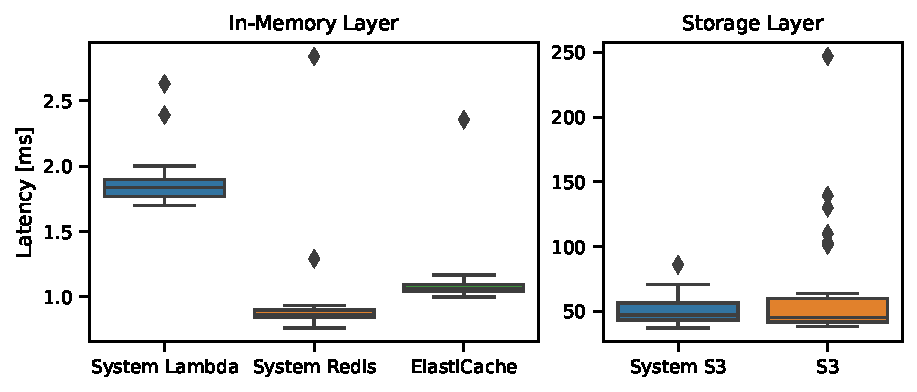
\includegraphics[width=\linewidth]{figures/proxy_latency_100B.pdf}
        \caption{Reverse Proxy latency measurement (100B).}
        \label{fig:proxy_latency_100B}
    \end{subfigure}
    
    \begin{subfigure}{.85\textwidth}
        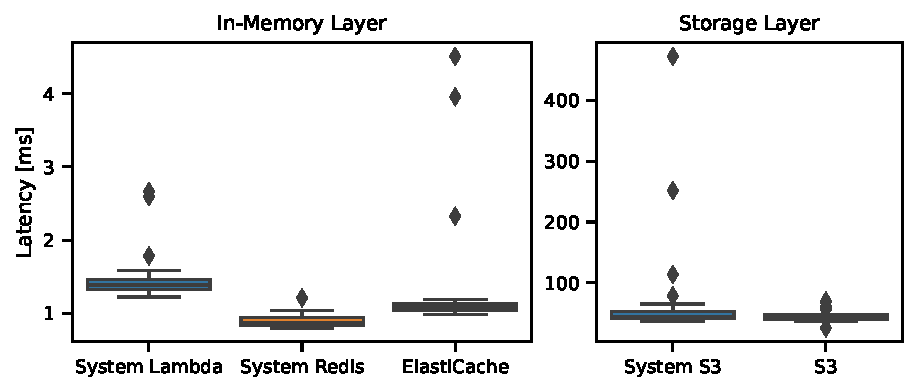
\includegraphics[width=\linewidth]{figures/proxy_latency_1KB.pdf}
        \caption{Reverse Proxy latency measurement (1KB).}
        \label{fig:proxy_latency_1KB}
    \end{subfigure}

    \begin{subfigure}{.85\textwidth}
        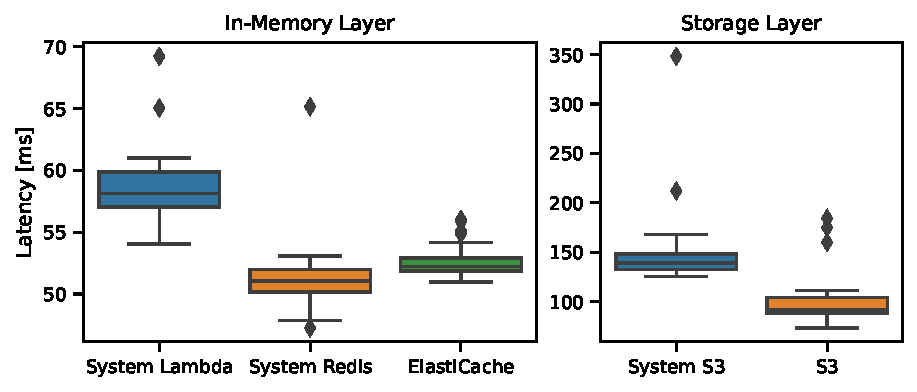
\includegraphics[width=\linewidth]{figures/proxy_latency_1MB.pdf}
        \caption{Reverse Proxy latency measurement (1MB).}
        \label{fig:proxy_latency_1MB}
    \end{subfigure}

    \caption{Measurement of request latency with respect to the reverse proxy. Latency includes the time it takes to process an API request within the AWS infrastructure on the reverse proxy. Each figure contains the measurements for specific object sizes. The left part contains the latency measurements for in-memory layers, while the right part describes the backend memory latency.}
    \label{fig:latency_proxy}
\end{figure}

\begin{figure}[pht!]
    \centering
    \begin{subfigure}{.85\textwidth}
        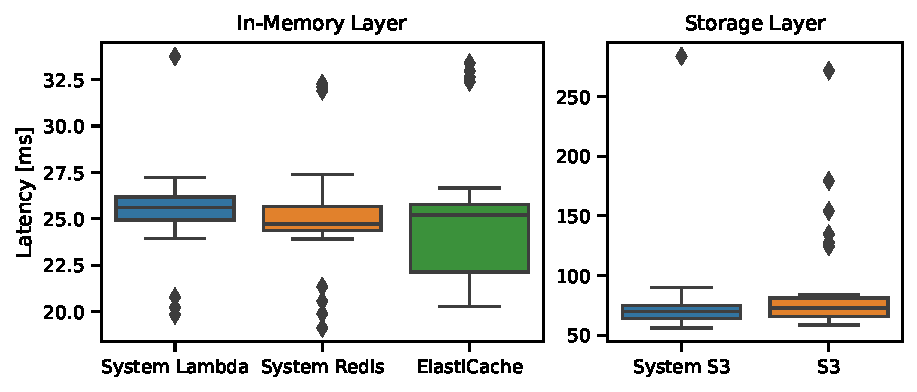
\includegraphics[width=\linewidth]{figures/client_latency_100B.pdf}
        \caption{End-to-end latency measurement (100B).}
        \label{fig:client_latency_100B}
    \end{subfigure}
    
    \begin{subfigure}{.85\textwidth}
        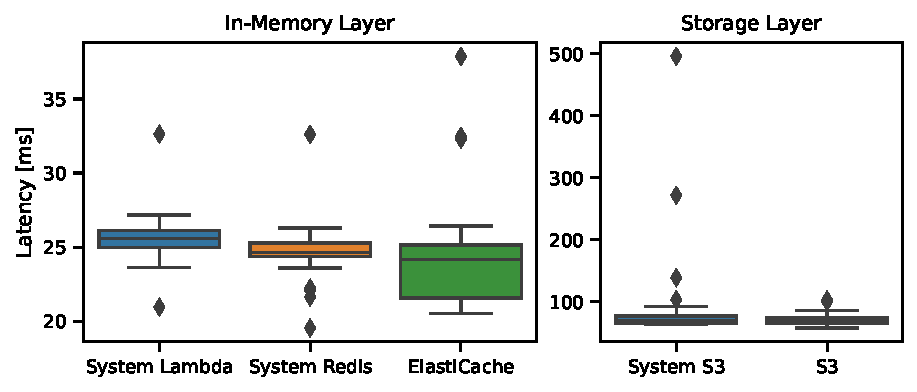
\includegraphics[width=\linewidth]{figures/client_latency_1KB.pdf}
        \caption{End-to-end latency measurement (1KB).}
        \label{fig:client_latency_1KB}
    \end{subfigure}

    \begin{subfigure}{.85\textwidth}
        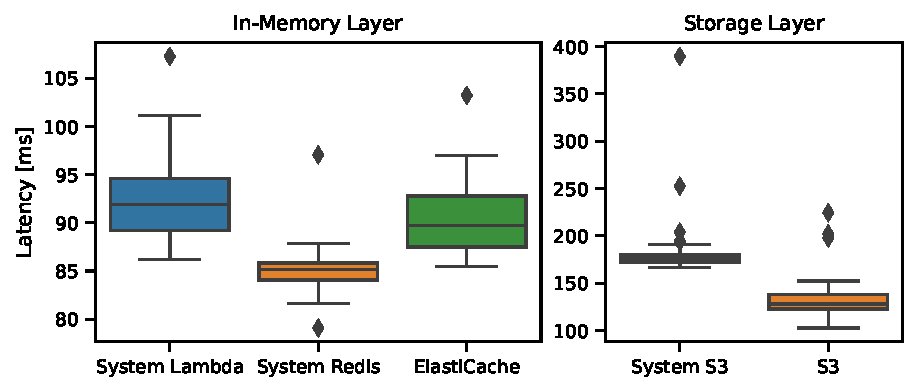
\includegraphics[width=\linewidth]{figures/client_latency_1MB.pdf}
        \caption{End-to-end latency measurement (1MB).}
        \label{fig:client_latency_1MB}
    \end{subfigure}

    \caption{Latency measurement in terms of total end-to-end latency measured on the client in our simulation. Each figure contains the measurements for specific object sizes. The left part contains the latency measurements for in-memory layers, while the right part describes the backend memory latency.}
    \label{fig:latency}
\end{figure}

% Each request is sent 30 times, while we wait 10 seconds between subsequent requests. We manually start the lambda runtime in our system using the control API and make sure that the same function is running for all 30 requests. We ignored the first measurement for the ElastiCache system because the lazy loading technique leads to AWS S3 access on the first request. The object is a simple random text file of a given size, and we repeated the experiment for different object sizes (100B, 1KB, and 1MB).

~\\
% Figure~\ref{fig:client_latency_100B},~\ref{fig:client_latency_1KB}, and~\ref{fig:client_latency_1MB} show the client-side measurements for the different object sizes, while Figure~\ref{fig:proxy_latency_100B},~\ref{fig:proxy_latency_1KB}, and~\ref{fig:proxy_latency_1MB} show the Gin API handler latency measurements from the respective proxy. 
Figure~\ref{fig:latency_proxy} shows the API handler latency measurements from the respective reverse proxy for the different object sizes, while Figure~\ref{fig:latency} shows the client-side end-to-end latency measurements. The results are consistent with the expectation of similar latencies for in-memory systems such as our self-hosted Redis layer, ElastiCache, and even our Lambda function achieves latency of the same order. As expected, the latency measurement for the persistent storage layer is about the same for our system as for a system without in-memory caching. 

~\\
The high latency of Internet traffic is evident when comparing the average latency from an in-memory endpoint for reverse proxy and client measurements. Thus, the average latency for processing an API request on our reverse proxy with the self-hosted Redis endpoint for the 100B object is less than one millisecond, as seen in Figure~\ref{fig:proxy_latency_100B}. In contrast, the average end-to-end latency for the same endpoint and object is about 25 ms, as seen in Figure~\ref{fig:client_latency_100B}. For endpoints with a higher latency on the reverse proxy side, this is no longer as serious in relation to each other. For the 100B object, the additional latency between reverse proxy and end-to-end measurements is approximately 24 ms, regardless of the endpoint. The same order of magnitude remains for the 1KB object. 

~\\
When we look at the reverse proxy measurements for the 1MB object, the storage layer latency increases similar to before between 100B and 1KB. In contrast, the latency increases drastically for each in-memory layer compared to the changes between 100B and 1KB. The reverse proxy copies the received object into the API response, which is a simple copy from the \code{io} package. The duration of the copy is most likely the reason for the increased latency as we approach much bigger objects of one MB. However, we still achieve better end-to-end latency for the in-memory layer than for the storage layer, although the difference is obviously much more significant for smaller objects, which we will focus on in further evaluations. Considering only the reverse proxy latency, the average latency of the in-memory layer for the 100B object is about 1.5 ms, while the memory layer is in the range of 50 ms, resulting in a $33.3\times$ faster in-memory caching retrieval with respect to the reverse proxy latency. Comparing the end-to-end latency, only about $3\times$ faster retrieval is achieved due to the additional latency of the Internet traffic.

\paragraph{Summary.} Both in-memory caching layers in our system achieve latency measurements on the same order of magnitude as ElastiCache. The slower layer S3 results in higher latency, which translates into a $33x$ speedup in terms of reverse proxy latency and a $3\times$ speedup for end-to-end latency due to the significant weight of additional Internet traffic latency. 

\section{Simulations}
\label{subsec:performance_evaluation}
With a better understanding of the latency measurements, we present the simulation results of our system with respect to the different traces used for the simulation. We start by testing our system on a trace modeling the same inter-arrival times of the requests as in the publicly available web server log described in Section~\ref{subsec:simulation_environment}. The extracted queries are for the most frequently queried object over the entire dataset, which includes the logs for one day. The duration of our simulation is one hour and includes all queries from the log for the object within the first hour. We assume the system administrator knows the average rate of requests per minute from the past, which is used for our system configurator. For this specific trace, it is about three requests per minute. For the sensitivity input, we run the simulation for three different values: two, three, and four.
\begin{figure}[t]
    \begin{center}
        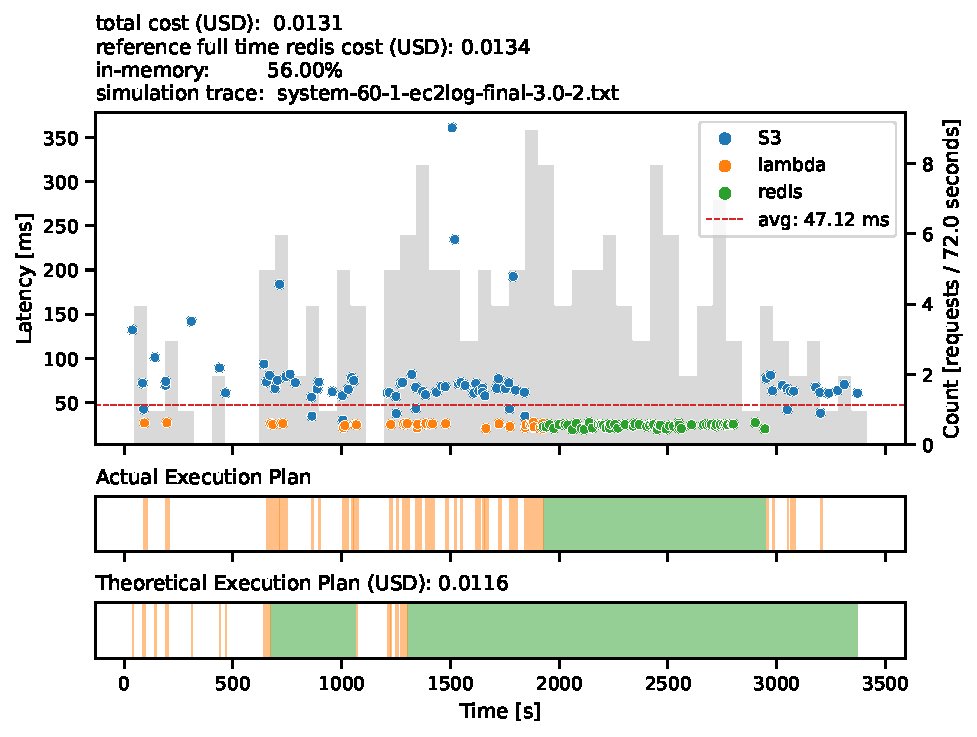
\includegraphics[width=0.8\textwidth]{figures/system-60-1-ec2log-final-3.0-2.pdf}
        \caption{Trace simulation on our system using the system configurator input (rate 3, sensitivity~2).}
        \label{fig:ec2log_3_2}
    \end{center}
\end{figure}

\paragraph{Figure Description.}
First, we provide an overview of the information presented in the simulation Figures such as Figure~\ref{fig:ec2log_3_2}. The x-axis represents the time during the simulation, while the y-axis represents the end-to-end latency measured on the client for each request. Each request is represented individually in the color of the particular endpoint that served the request. The bar chart in the background illustrates the workload distribution with the corresponding bucket size and requests per bucket indicated on the second y-axis on the right. The second subplot is a visualization of the currently active caching layer during the simulation, while the subplot below it visualizes the decision of our offline endpoint scheduler.

\begin{figure}[t]
    \begin{center}
        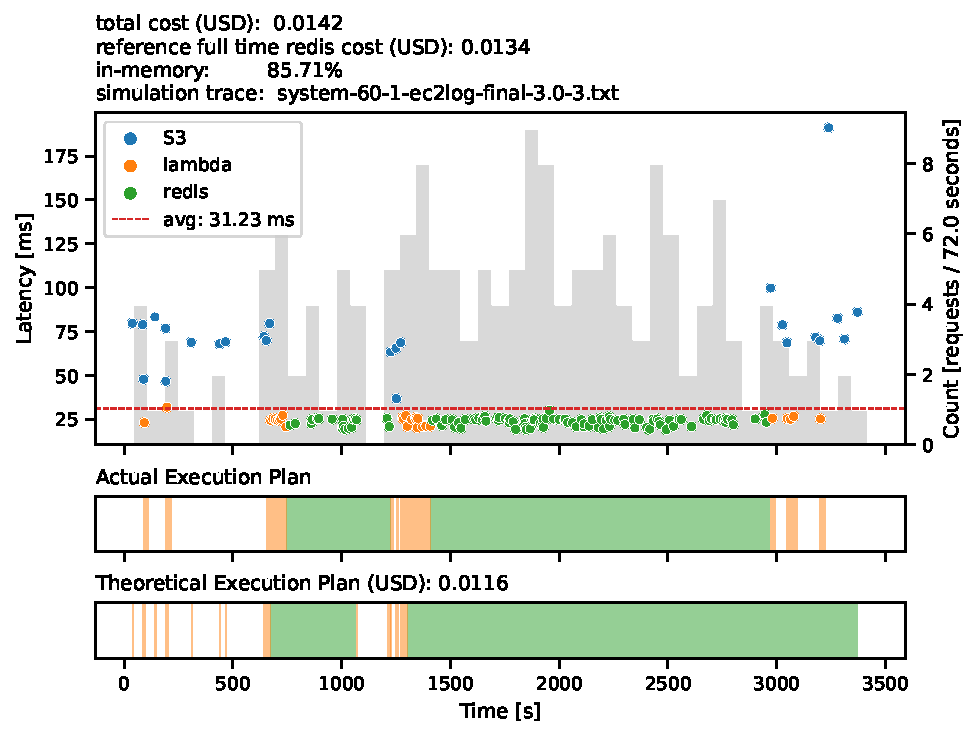
\includegraphics[width=0.8\textwidth]{figures/system-60-1-ec2log-final-3.0-3.pdf}
        \caption{Trace simulation on our system using the system configurator input (rate 3, sensitivity~3).}
        \label{fig:ec2log_3_3}
    \end{center}
\end{figure}

\begin{figure}[t]
    \begin{center}
        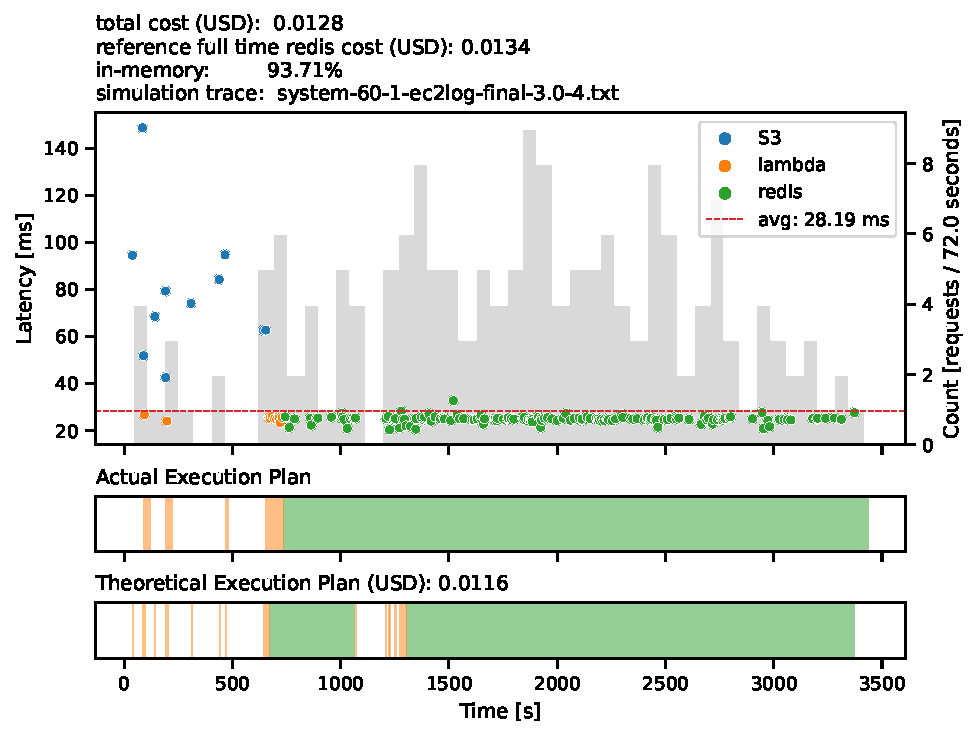
\includegraphics[width=0.8\textwidth]{figures/system-60-1-ec2log-final-3.0-4.pdf}
        \caption{Trace simulation on our system using the system configurator input (rate 3, sensitivity~4).}
        \label{fig:ec2log_3_4}
    \end{center}
\end{figure}

\paragraph{Sensitivity Value.}
The first obvious observation is the strong dependency of system parameters and the resulting endpoint decision-making process as shown in Figure~\ref{fig:ec2log_3_2},~\ref{fig:ec2log_3_3}, and~\ref{fig:ec2log_3_4}. While the rate remains the same in these simulation results, only varying the sensitivity value results in a completely different system at first glance. During the development, we started with fixed system parameters. The first few experiments clearly showed the need for a more dynamically configurable system, which led to the integration of the system configurator. As we increase the sensitivity, we achieve a higher in-memory percentage as expected. So for sensitivity two, only 56\% of the requests are served by either our Lambda runtime or the Redis layer, for sensitivity three we achieve 85.71\%, and for four we even reach 93.71\%. 

~\\
Initially, one would think the higher the sensitivity value, the higher the cost, which is the case for the first two. However, the highest sensitivity value in our experiments is also the experiment with the lowest cost. The reason for this is the more expensive serverless layer compared to the self-hosted Redis, which is used less often than the higher the sensitivity value, as one can easily see in the actual execution plan in the Figures~\ref{fig:ec2log_3_2} to~\ref{fig:ec2log_3_4}. The simulation using a sensitivity value of four achieves an in-memory percentage of 93.71\% and is even cheaper than an always running self-hosted Redis instance of the same type used in our system, but keep in mind that this instance would reach 100\%. 

\paragraph{Offline Endpoint Scheduler.}
When we look at the theoretical execution plan obtained by our offline endpoint scheduler, it is not surprising that the algorithm with the trace known in advance would achieve 100\% in-memory percentage at a lower cost than our system. A more detailed analysis of our endpoint scheduler is presented in the next section. 

\paragraph{Comparison Systems.}
Figure~\ref{fig:comparison_systems} shows the results of the same simulation for the two comparison systems using only S3 and ElastiCache, with lazy loading resulting in S3 access for the first request in ElastiCache. As already explained in the previous section, the end-to-end latencies for the in-memory layer and the storage layer are in the same order of magnitude. ElastiCache achieves an average end-to-end latency of 24.03 ms. Our system with sensitivity 4 achieves a comparable average of 28.19 ms, but as soon as the sensitivity decreases, the average end-to-end latency increases due to the increased number of S3 accesses. A system without in-memory caching as in Figure~\ref{fig:ec2log_s3} obviously achieves the lowest cost, while the price difference for ElastiCache compared to a self-hosted Redis instance is also no surprise but simply a reflection of the price difference of the instance type based on the fully managed service.

% The trace includes 174 requests during the one-hour simulation. So we are nowhere near the point where self-hosted Redis can be cheaper than the cost of S3 requests, as discussed in section~\ref{subsec:comparison_systems}.

\begin{figure}[t]
    \centering
    \begin{subfigure}{.78\textwidth}
        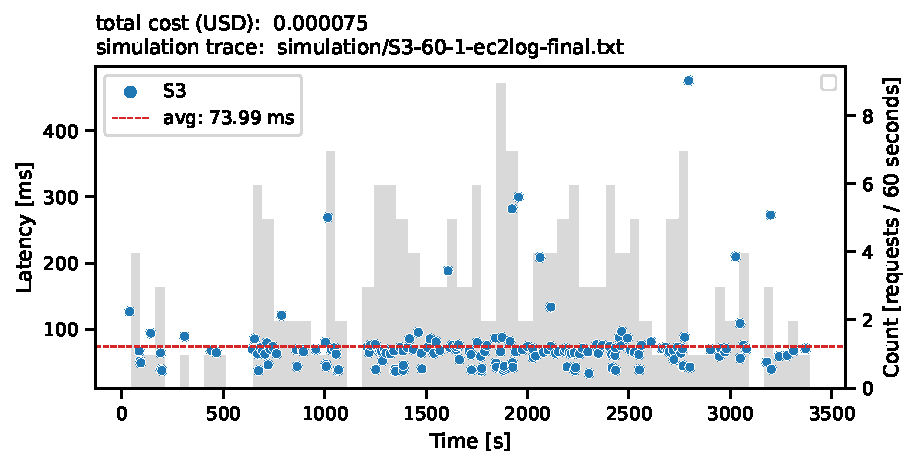
\includegraphics[width=\linewidth]{figures/S3-60-1-ec2log-final.pdf}
        \caption{Simulation on AWS S3 only.}
        \label{fig:ec2log_s3}
    \end{subfigure}
    \begin{subfigure}{.78\textwidth}
        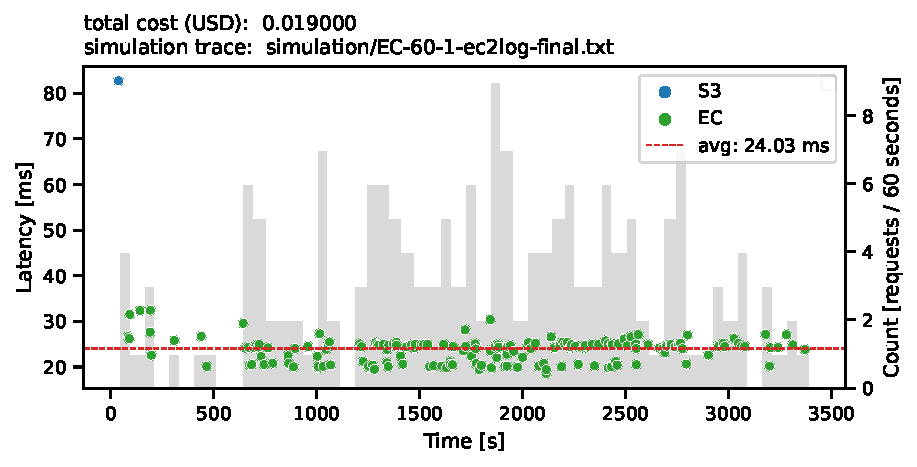
\includegraphics[width=\linewidth]{figures/EC-60-1-ec2log-final.pdf}
        \caption{Simulation on AWS ElastiCache (EC in the figure).}
        \label{fig:ec2log_ec}
    \end{subfigure}
    \caption{Results of the one-hour simulation based on the web server log for the two comparison systems.}
    \label{fig:comparison_systems}
\end{figure}

\paragraph{Varying Workload.}
In order to run our simulation with different traces, we add the method described in Section~\ref{subsec:simulation_environment} to generate traces using a Poisson process. The previous trace does not exactly correspond to a Poisson process, but it also contains an approximately constant average rate of requests. Therefore, we use this method to examine the results for different Poisson process parameters and explore the usability of our system. From the beginning, the goal of our system was to explore the possibilities of integrating the serverless platform as a caching layer into a Redis-based system. The goal was not to design a system that could handle every possible workload, as the design of our system stops making sense once the average request rate is high enough since a constantly running Redis instance will always beat our system in terms of cost at that point. At the same time, a reactive system is useless for workloads with a low average number of requests. More precisely, the advantage of a more expensive and faster reacting serverless layer is not helpful. The simulation results for the Poisson process-based traces in Figures~\ref{fig:poisson_3_23} to~\ref{fig:poisson_4_45} help to understand the design limitations of our system, which we discuss in more detail in the next section with a closer look at our endpoint scheduler. Nevertheless, these results help us understand the design of our system and the use cases where we can actually benefit from a reactive in-memory caching design, as described in Section~\ref{subsec:peak_workload}.

\begin{figure}[pht!]
    \centering
    \begin{subfigure}{.8\textwidth}
        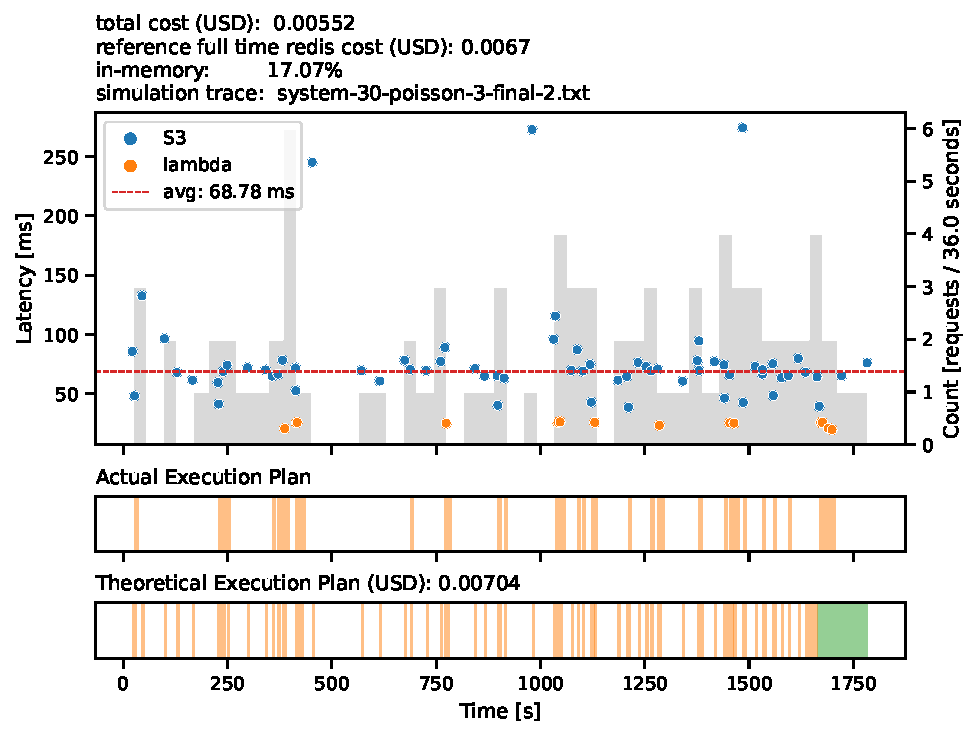
\includegraphics[width=\linewidth]{figures/system-30-poisson-3-final-2.pdf}
        \caption{System configurator used a sensitivity value of 2.}
        \label{fig:poisson_3_2}
    \end{subfigure}
    \begin{subfigure}{.8\textwidth}
        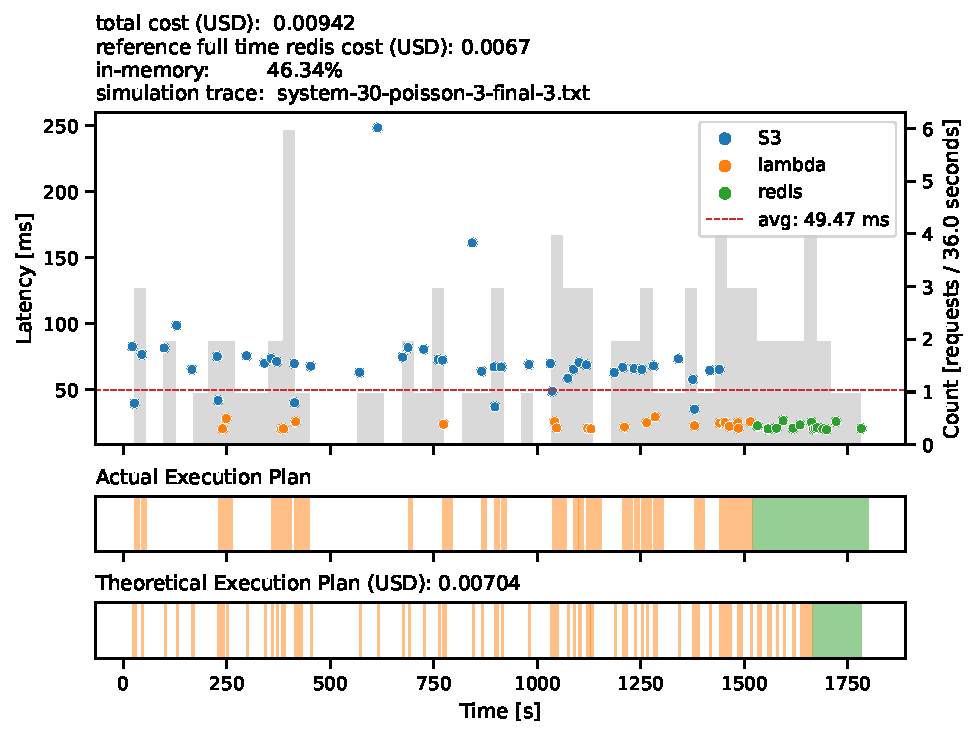
\includegraphics[width=\linewidth]{figures/system-30-poisson-3-final-3.pdf}
        \caption{System configurator used a sensitivity value of 3.}
        \label{fig:poisson_3_3}
    \end{subfigure}
    \caption{Simulations on our system using the rate 3 for the system configurator as the workload is derived as a Poisson process with rate 3. Results for sensitivity values 2 and 3.}
    \label{fig:poisson_3_23}
\end{figure}

\begin{figure}[pht!]
    \centering
    \begin{subfigure}{.8\textwidth}
        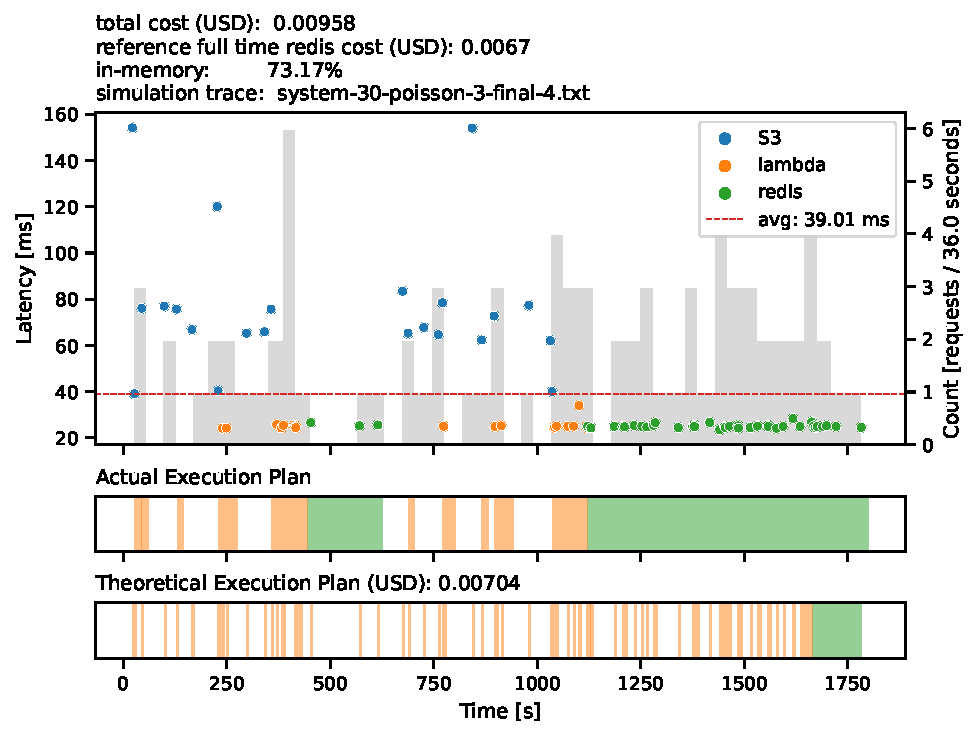
\includegraphics[width=\linewidth]{figures/system-30-poisson-3-final-4.pdf}
        \caption{System configurator used a sensitivity value of 4.}
        \label{fig:poisson_3_4}
    \end{subfigure}
    \begin{subfigure}{.8\textwidth}
        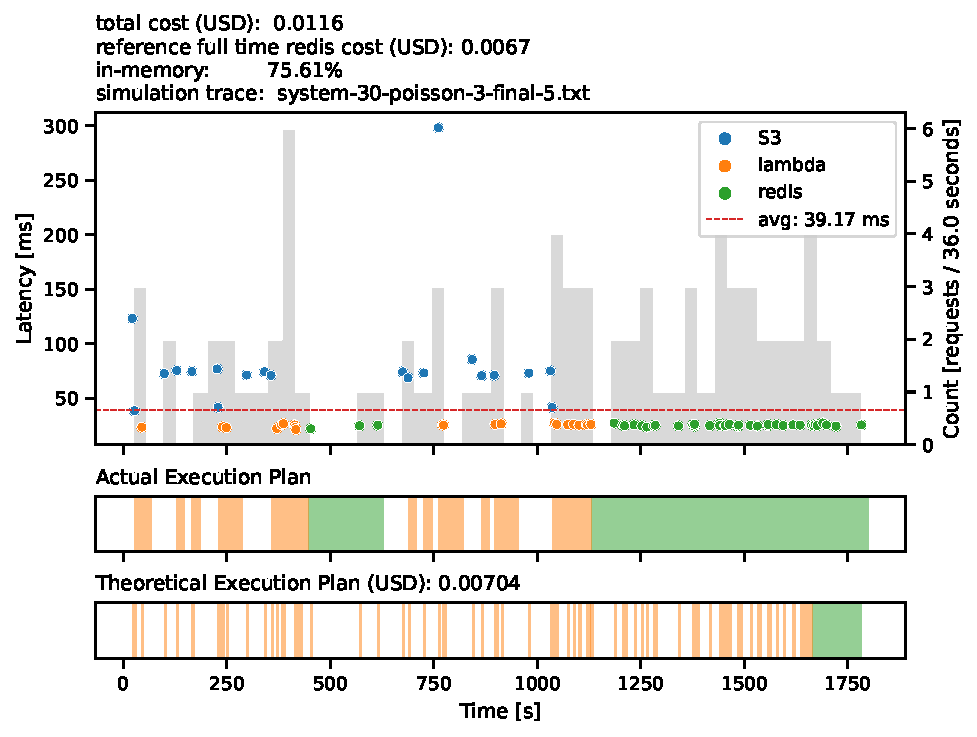
\includegraphics[width=\linewidth]{figures/system-30-poisson-3-final-5.pdf}
        \caption{System configurator used a sensitivity value of 5.}
        \label{fig:poisson_3_5}
    \end{subfigure}
    \caption{Simulations on our system using the rate 3 for the system configurator as the workload is derived as a Poisson process with rate 3. Results for sensitivity values 4 and 5.}
    \label{fig:poisson_3_45}
\end{figure}

\begin{figure}[pht!]
    \centering
    \begin{subfigure}{.8\textwidth}
        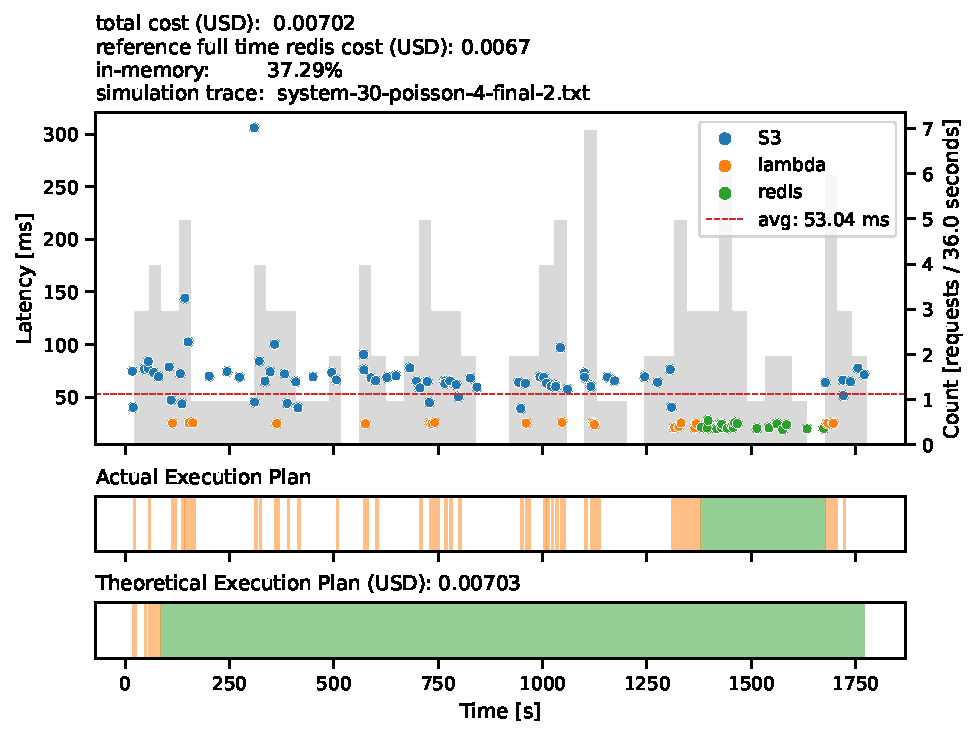
\includegraphics[width=\linewidth]{figures/system-30-poisson-4-final-2.pdf}
        \caption{System configurator used a sensitivity value of 2.}
        \label{fig:poisson_4_2}
    \end{subfigure}
    \begin{subfigure}{.8\textwidth}
        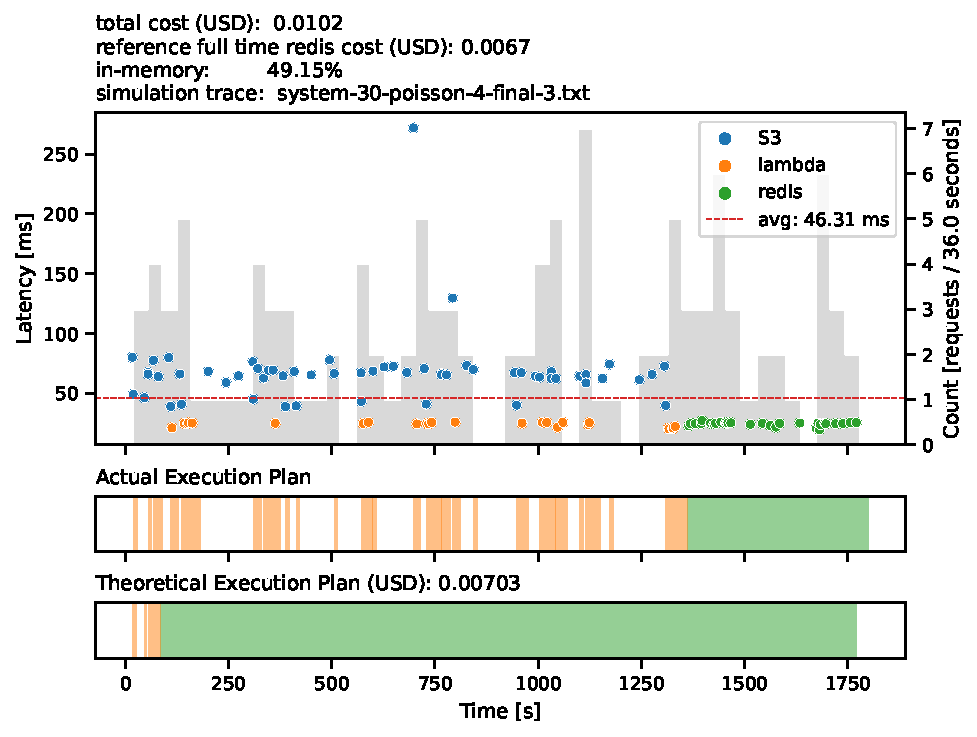
\includegraphics[width=\linewidth]{figures/system-30-poisson-4-final-3.pdf}
        \caption{System configurator used a sensitivity value of 3.}
        \label{fig:poisson_4_3}
    \end{subfigure}
    \caption{Simulations on our system using the rate 4 for the system configurator as the workload is derived as a Poisson process with rate 4. Results for sensitivity values 2 and 3.}
    \label{fig:poisson_4_23}
\end{figure}

\begin{figure}[pht!]
    \centering
    \begin{subfigure}{.8\textwidth}
        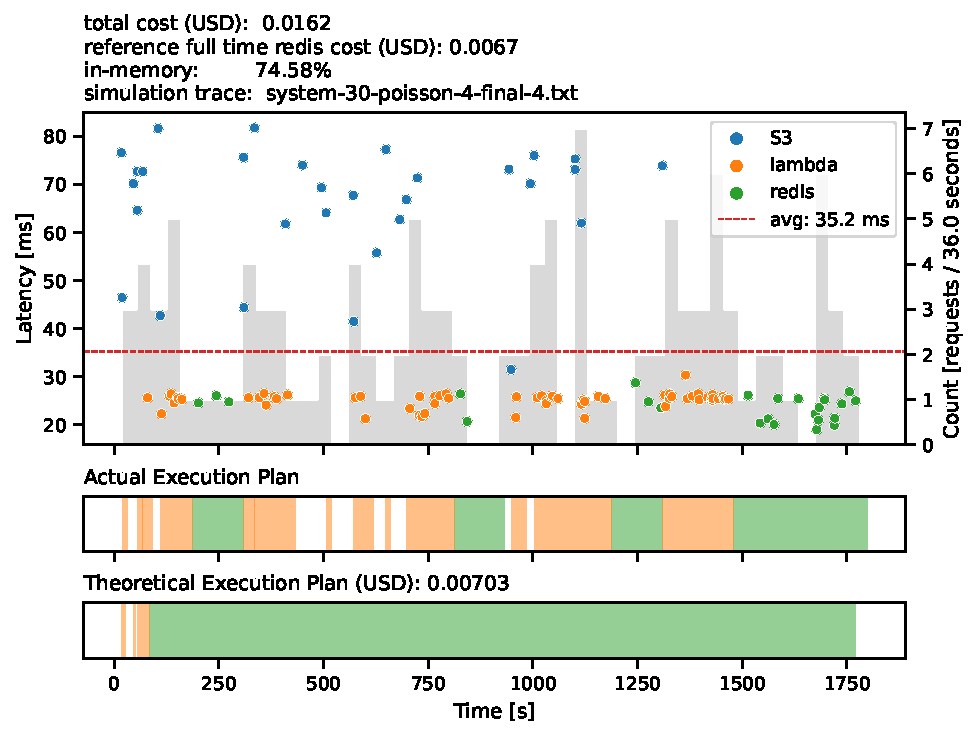
\includegraphics[width=\linewidth]{figures/system-30-poisson-4-final-4.pdf}
        \caption{System configurator used a sensitivity value of 4.}
        \label{fig:poisson_4_4}
    \end{subfigure}
    \begin{subfigure}{.8\textwidth}
        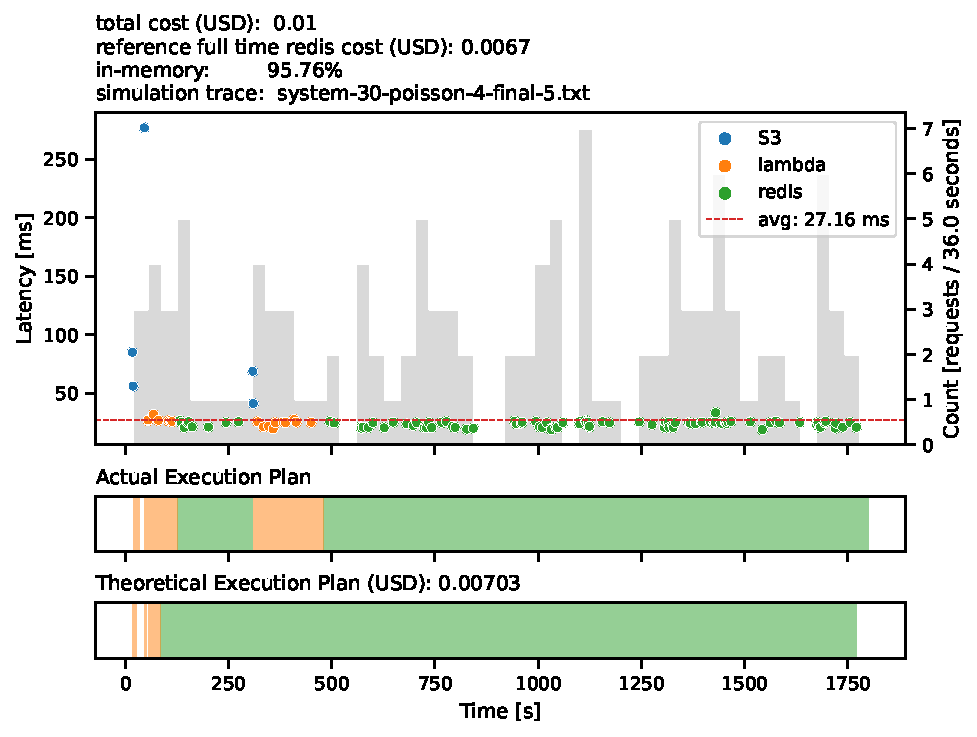
\includegraphics[width=\linewidth]{figures/system-30-poisson-4-final-5.pdf}
        \caption{System configurator used a sensitivity value of 5.}
        \label{fig:poisson_4_5}
    \end{subfigure}
    \caption{Simulations on our system using the rate 4 for the system configurator as the workload is derived as a Poisson process with rate 4. Results for sensitivity values 4 and 5.}
    \label{fig:poisson_4_45}
\end{figure}

\paragraph{Summary.}
We use the simulations to explore the usability of our system. The close dependence between the system parameters and the workload in terms of in-memory percentage and cost is quickly apparent. The results show some clear limitations of our system for use as a cost-effective caching system for general workloads. For example, either response time does not matter if the frequency of requests is too low, or a reactive design is meaningless if caching is desired all the time. The results in this section form the basis for discussing our endpoint scheduler in the next section.

\section{Endpoint Scheduler}
\label{sec:endpoint_scheduler}
% analyze the behaviour and performance of our endpoint scheduler
% explain their impact on the system with trace examples and actual simulations.
% conclusion should be that the design our system target to enhance the speedup to make in-memory caching available -> so unexpected peak workloads are of interest
The previous section briefly introduced the strong dependence of the system parameters and the resulting endpoint decision process on our endpoint scheduler. We use the simulations presented to shed more light on this dependence. For the purposes of this discussion, the system parameters for the specific inputs to the system configurator are shown in Table~\ref{tab:system_configurator}.

\paragraph{System Parameters in Action.}
The independent parameters \emph{lambdaWindowElements} and \emph{redisThreshold} determine the number of requests required to be resolved by the previous layer within specific time duration to transition to the new layer and therefore to a new state as shown in Figure~\ref{fig:endpoint_scheduler}. The mentioned time duration is the part for which our system configurator derives different values depending on the input. For example, for \emph{lambdaWindowElements}, the requests must be received within the time window specified by the \emph{lambdaThreshold}, while \emph{redisThreshold} is linked to the \emph{TICK} duration, which determines how long the Lambda runtime will run. The last system parameter \emph{redisUtilization} specifies the time in which the last five requests for our Redis layer must have arrived; otherwise, the Redis layer is stopped. Therefore, this parameter represents the tolerance of whether we keep our Redis layer running. Thus, depending on these parameters, our endpoint scheduler's trade-off in maintaining in-memory caching layers versus cost savings is clearly evident.

~\\
So as we increase the \emph{TICK} duration, the possibility of two subsequent requests being forwarded to the same Lambda runtime invocation increases. Since the \emph{TICK} duration is also used to extend the timeout functionality on our Lambda runtime, a larger \emph{TICK} duration also increases the probability of reaching the \emph{redisThreshold} and thus switching to the Redis-based part of our system. The downside of increasing the \emph{TICK} duration is the increased cost of the longer-running Lambda layer. The \emph{lambdaThreshold} defines the granularity at which our system actually starts any state transitions, so if we never receive two subsequent requests within this duration, our system is stuck in the \textsc{S3} state and will never make use of the in-memory caching layers. This duration should help anticipate the arrival of multiple requests in the future. At this point, we want to deploy in-memory caching while not being too reactive and starting the Lambda layer every time a single request arrives. With a general understanding of our system parameters, we now look at the simulation results with a focus on the endpoint scheduler.

\begin{table*}[t]
    \centering
    \ra{1.1}
        \begin{tabular}{ @ {} r r c r r r @ {}}
        \toprule
        \multicolumn{2}{c}{Configurator Input} & \phantom{abc} & \multicolumn{3}{c}{System Parameters} \\
        \cmidrule{1-2} \cmidrule{4-6}
        rate  & sensitivity && \emph{TICK} & \emph{lambdaThreshold} & \emph{redisUtilization} \\
        \midrule
        3 & 2 && 8s  & 16s & 2m20s \\
        3 & 3 && 12s  & 24s & 2m40s \\
        3 & 4 && 16s  & 32s & 3m00s \\
        4 & 2 && 6s  & 12s & 1m45s \\
        4 & 3 && 9s  & 18s & 2m00s \\
        4 & 4 && 12s & 24s & 2m15s \\
        6 & 2 && 4s  & 8s & 1m10s \\
        6 & 3 && 6s & 12s & 1m20s \\
        6 & 4 && 8s & 16s & 1m30s \\
        9 & 4 && 5s & 10s & 1m00s \\
        \bottomrule
        \end{tabular}
    \caption{Comparison of different system parameters depending on the system configurator input. Two system parameters are chosen independently of the input and are therefore omitted from the table. The \emph{lambdaWindowElements} is set to 2 and the redisThreshold to 4.}
    \label{tab:system_configurator}
\end{table*}

\paragraph{Simulation Analysis.}
The results for the web server log trace experiments, which all used a rate of 3 for the system configuration, vary widely. This is due to the changing system parameters caused by the varying sensitivity value. Figure~\ref{fig:ec2log_3_2} shows that the duration of \emph{lambdaThreshold} is low enough to trigger the transition to Lambda multiple times. However, the duration of \emph{TICK} appears to be too low to capture many requests and also results in only a single transition to the Redis-based system. So our system often starts the Lambda layer without serving many requests from it, which causes the higher total costs compared to the simulation using sensitivity three in Figure~\ref{fig:ec2log_3_3}. A closer look at the cost composition clearly confirms our assumption. The total billed duration for the Lambda layer is about 394 seconds compared to the 556 seconds for the lower sensitivity value. Thus, for sensitivity value two, \$0.00929 of total \$0.0131 is spent on the runtime duration for the serverless layer alone, while for sensitivity value three, only \$0.0066 of \$0.0142 is spent. The higher total cost for the higher sensitivity value is thus caused by the much longer runtime of the less expensive Redis layer, which also explains the much higher in-memory percentage. The influence of \emph{redisUtilization} becomes clear when we compare Figure~\ref{fig:ec2log_3_3} and Figure~\ref{fig:ec2log_3_4}. In the beginning, they are quite similar, but the lower \emph{redisUtilization} causes the Redis instance to be shut down, while a higher sensitivity value keeps the Redis instance alive in the same scenario, resulting in a higher in-memory percentage and lower overall cost by avoiding the more expensive Lambda runtime which is used almost immediately after the instance is shut down to transition back to the Redis state.

\paragraph{Endpoint Scheduler Limitations.}
We experiment with the Poisson process-based traces to evaluate the endpoint scheduler for multiple traces and thus different workload characteristics. Our expectation regarding the limited usability of our system with a more or less constant request rate modeled as a Poisson process was quickly confirmed. The results in terms of cost efficiency were poor compared to the web server log trace. The theoretical execution plan provides an interesting insight for this discussion. Once the rate is too low, our offline endpoint scheduler basically avoids using the Redis-based layer and uses only the serverless layer, as shown for the Poisson process trace for rate three in Figure~\ref{fig:poisson_3_23}. The result for our offline endpoint scheduler is exactly the opposite if we increase the Poisson process rate to four: it keeps the Redis layer all the time while using the Lambda layer only at the beginning, as shown in Figure~\ref{fig:poisson_4_23}. Increasing the sensitivity does lead to a higher percentage of in-memory with the consequence of higher costs. However, due to the constant request rate, we never really benefit from the reactive design of our system. 

~\\
Compared to the web server log, where our system saves costs in the first ten minutes because almost no requests arrive, and thus no in-memory layer is urgently needed. Thus, if we reconsider our interpretation of the similarity of the web server log to a Poisson process, we see the significance of the two peaks. The simulation in Figure~\ref{fig:ec2log_3_3} marks these peaks during the periods when our system is running the Redis layer. The break between the peaks is very short, so we can save costs by running the Redis layer between these peaks, as is the case with the higher sensitivity value. In summary, the design of our system targets peak workloads where we can actually benefit from the responsiveness and design of our system. Attempting to build a general caching system with our system configurator is already severely compromised by design and does not appear to be goal-oriented. For this reason, we are focusing for now on workload peaks where the design of our system is critical.

\paragraph{Summary.}
A closer look at the endpoint scheduler and its system parameters in the context of the simulations helps to understand the tight dependency mentioned in the previous section. The current design of our system is understandably not for general workloads, which is nicely emphasized by the offline endpoint scheduler for the Poisson process traces. The reactive design of our system is clearly designed for bursty workloads, which will be discussed in the next section. 

\section{Bursty Workload}
\label{subsec:peak_workload}

\begin{figure}[t]
    \begin{center}
        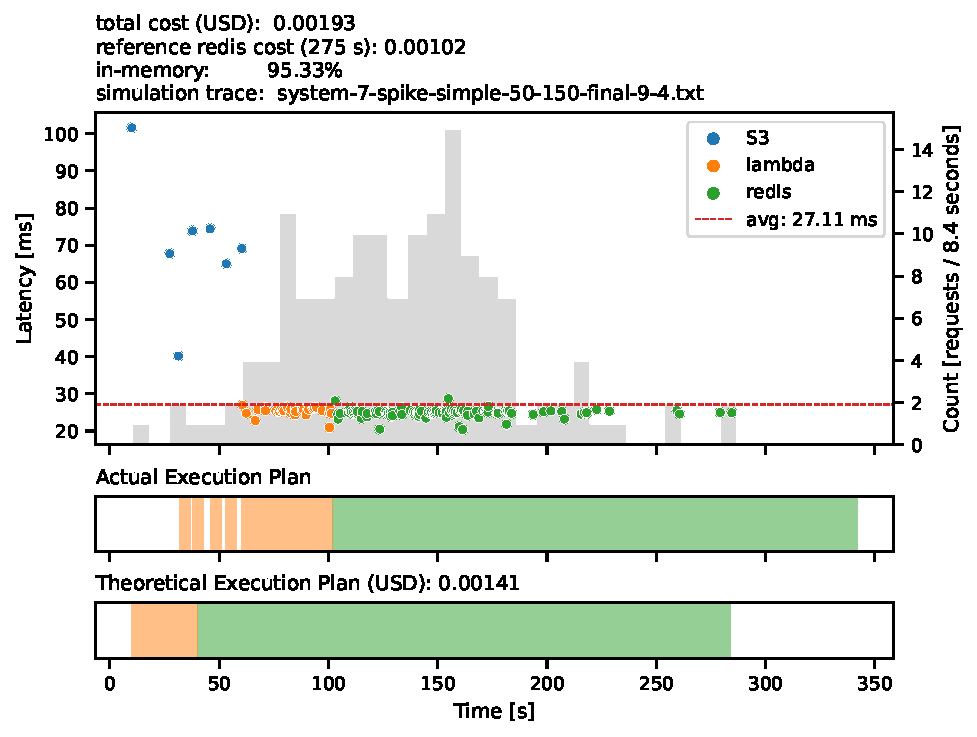
\includegraphics[width=0.8\textwidth]{figures/system-7-spike-simple-50-150-final-9-4.pdf}
        \caption{The arrival times for 150 requests were taken from a normal distribution with a standard deviation of 50 seconds to simulate a peak load on our system.}
        \label{fig:spike_1}
    \end{center}
\end{figure}

\begin{figure}[t]
    \begin{center}
        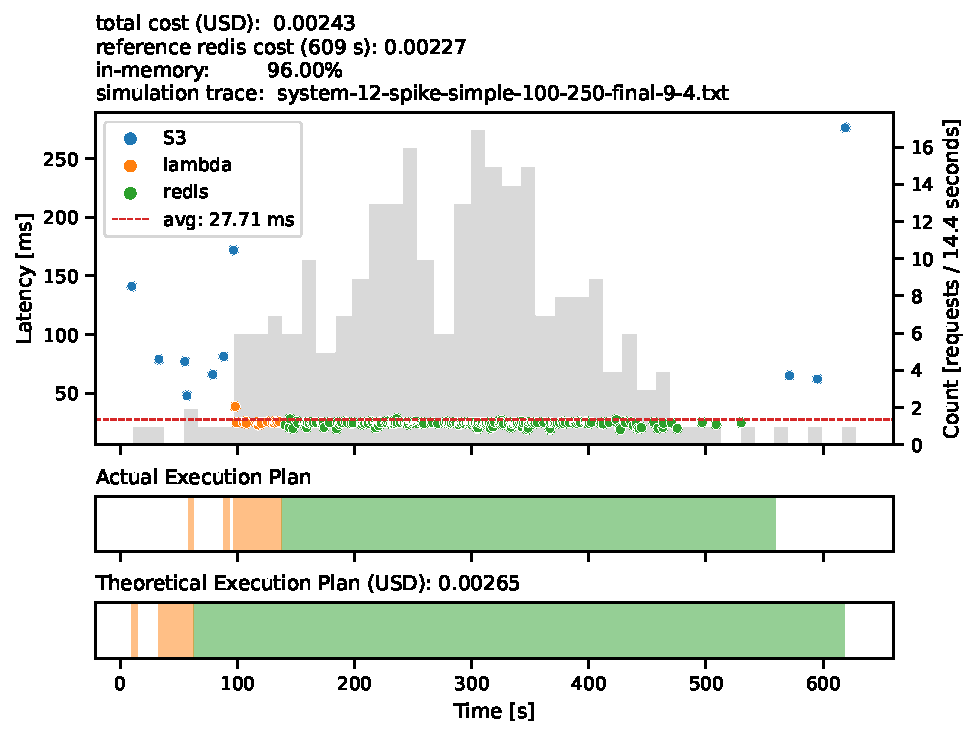
\includegraphics[width=0.8\textwidth]{figures/system-12-spike-simple-100-250-final-9-4.pdf}
        \caption{The arrival times for 250 requests were taken from a normal distribution with a standard deviation of 100 seconds to simulate a peak load on our system.}
        \label{fig:spike_2}
    \end{center}
\end{figure}
When focusing on burst workloads, we can safely assume that at some point, enough requests are received to trigger the state transition on our endpoint scheduler. Therefore, the system parameters become drastically less important. Nevertheless, the system parameters still play an important role depending on the tail distribution of the peak since they indicate how fast our system reacts to an approaching spike and how it behaves when the peak drops. To investigate more on the behavior of our system during spike workloads, we run additional experiments using the \emph{spike-simple} method described in Section~\ref{subsec:simulation_environment}. It uses a normal distribution to model the spike while the simulation duration is limited to the actual samples from the distribution. In the context of these experiments, we assume that the arrival time of the spike is unknown while the rate during the spike is high enough so that a Redis instance is always more cost-effective than Lambda. While we vary the duration of these spikes by taking more samples from a normal distribution with a higher standard deviation, we focus on spikes that last less than one hour. Therefore, comparing our system with ElastiCache is not of much interest due to the billing granularity of node hours. Nevertheless, when we look at the arrival frequency of these spikes at the end, we include ElastiCache again in our discussion. 

\paragraph{Perfect Automation Process.}
Remember the perfect automation process for a self-hosted Redis-based system, described at the end of Section~\ref{subsec:comparison_systems}. The perfect automation process provides a lower bound with respect to cost for a Redis-based system where the instance is exactly running as soon as we receive the first request and shut down after the last request was received. This would require knowing the trace in advance and starting the instance at just the right time so that it does not run too early, which would add some overhead. The baseline provided by this comparison system helps evaluate the cost-effectiveness of our system for these experiments. Thus, the reference costs shown in the charts are no longer a full-time Redis instance but only include the billed duration between the first and the last request.

\begin{figure}[t]
    \begin{center}
        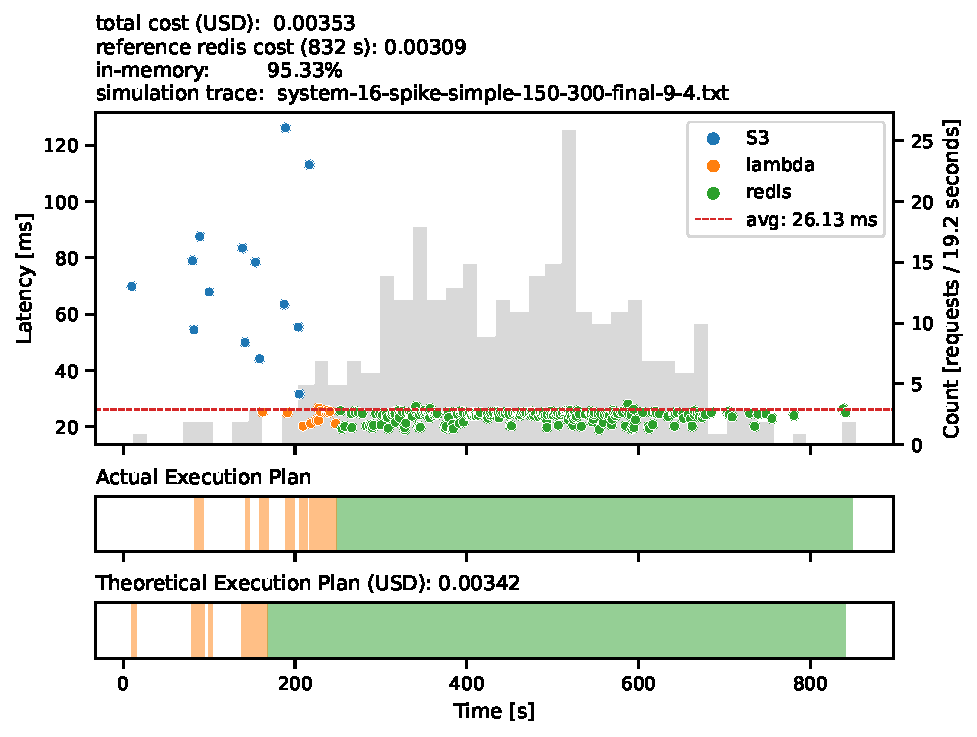
\includegraphics[width=0.8\textwidth]{figures/system-16-spike-simple-150-300-final-9-4.pdf}
        \caption{The arrival times for 300 requests were taken from a normal distribution with a standard deviation of 150 seconds to simulate a peak load on our system.}
        \label{fig:spike_3}
    \end{center}
\end{figure}

\begin{figure}[t]
    \begin{center}
        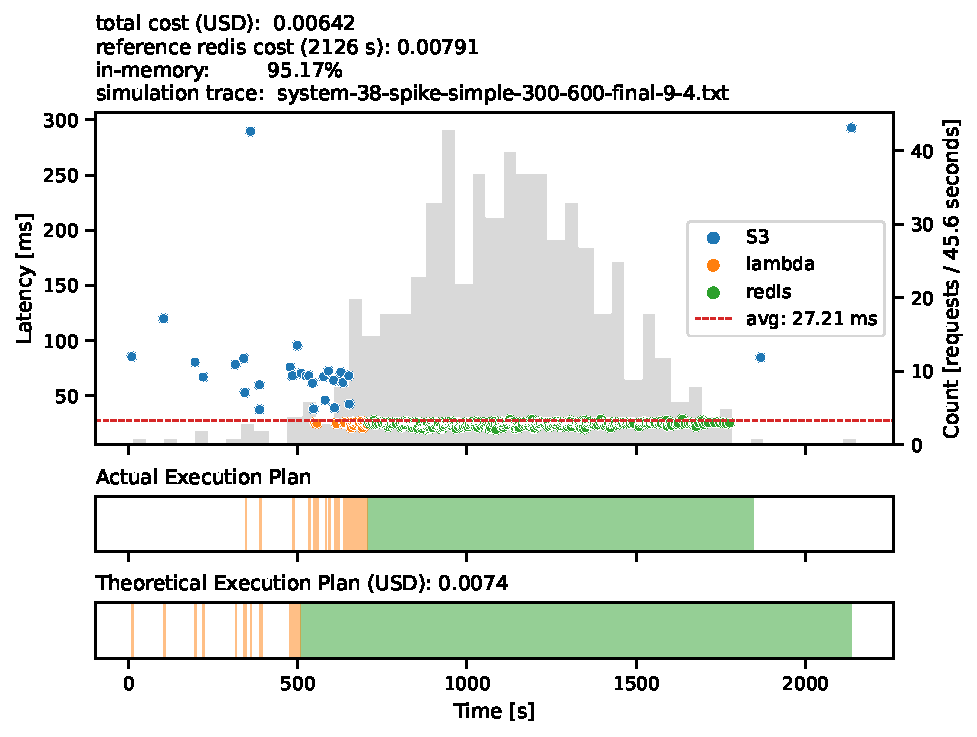
\includegraphics[width=0.8\textwidth]{figures/system-38-spike-simple-300-600-final-9-4.pdf}
        \caption{The arrival times for 600 requests were taken from a normal distribution with a standard deviation of 300 seconds to simulate a peak load on our system.}
        \label{fig:spike_4}
    \end{center}
\end{figure}

\paragraph{Simulation Results.}
First, we present the results for different spike durations where we used the system parameters shown in the last row of Table~\ref{tab:system_configurator}. The way our system configurator is designed is not really intended to optimize the performance of our system with respect to spike workloads. For this reason, we fix the system parameters for these experiments and discuss their effects at the end and consider how they could be improved. 

~\\
We find that we achieve a similar in-memory percentage between 95\% and 96\% for each peak, with a big difference when we compare the actual cost of our system to the Redis-based reference system. Thus, for a short peak as in Figure~\ref{fig:spike_1}, our system is almost twice as expensive, while for the longer-lasting peak as in Figure~\ref{fig:spike_4} we are even cheaper. An important point regarding cost is the usage of the serverless layer, which is a less cost-efficient in-memory caching layer than the self-hosted Redis instance. While the number of calls and the total runtime of our Lambda layer still depends on the actual distribution of requests arriving at our system, their proportional share in the total cost decreases significantly. For the simulation in Figure~\ref{fig:spike_1}, the billed Lambda duration is responsible for 53\% of the total cost, while the percentage is between 33-36\% for the other three experiments. 

~\\
So we can argue that our system is less cost-effective with a short peak duration, but on the other hand, handling a short peak duration with an automation process is even more difficult. So if the automation process only responds by starting the Redis instance as soon as the first request comes in, this could result in several EC2 billing minutes where only a single request is received and no actual peak. When a peak comes in, we miss a large portion of the peak while the automation process starts the instance. The fraction missed by a reactive automation process decreases as the duration of the spike increases, but this leads to another interesting discussion about the tail distribution of the peaks. 

\paragraph{Tail Distribution.}
So while a perfect automation process for self-hosted Redis would achieve 100\% in-memory caching, it runs at the beginning of the peak and continues to run until the last request is received. This results in a total runtime of 2126 seconds for the Redis reference instance in Figure~\ref{fig:spike_4} while the combined runtime of our caching layers totals only 1270 seconds. We thus achieve an in-memory percentage of 95.17\%, while running the in-memory layer only 60\% of the time. 

~\\
This effect is somewhat limited to the shorter peaks by our current system configurator's previously mentioned adjustability limitation. Thus, with the system parameters, we can control our system's responsiveness and set the tolerance threshold for shutting down a running in-memory layer. While the responsiveness is quite satisfying with respect to the experiments, we notice a problem in the current configurator design when handling short peak durations. Recall that our endpoint scheduler reevaluates once a minute if the Redis layer should be kept alive using the \emph{redisUtilization} system parameter. In the case of a short spike duration, the granularity at which we do this check is obviously a big problem, as shown in Figure~\ref{fig:spike_1}. However, the problem we mentioned regarding the system configurator is related to the way we derive the \emph{redisUtilization}. Because for a short spike duration, we want to keep the other system parameters but reduce the \emph{redisUtilization} to react faster when the end of the spike is approaching, which is currently not possible with our system configurator.

\begin{table}[t]
    \centering
    \ra{1.2}
        \begin{tabular}{ @ {} r c r r c r r @ {} }
        \toprule
        \multicolumn{1}{c}{} & \phantom{abc }& \multicolumn{2}{c}{Self-Hosted Redis} & \phantom{abc} & \multicolumn{2}{c}{AWS ElastiCache} \\
        \cmidrule{3-4} \cmidrule{6-7}
        spike duration &&  spikes  & hourly coverage &&  spikes  & hourly coverage \\
        \midrule
        275s && 6 & $45\%$ && 9 &  $68\%$ \\
        609s && 5 & $84\%$ && 7 & $>100\%$ \\
        832s && 3 & $69\%$ && 5 &  $>100\%$ \\
        2126s && 2 & $>100\%$ && 2 & $>100\%$ \\
        \bottomrule
        \end{tabular}
    \caption{For each experiment in this section, we give the maximum number of spikes that can occur during an hour so that our system still results in a lower cost than the two comparison systems. We also calculate the percentage of an hour that the number of spikes could span without overlapping.}
    \label{tab:spikes}
\end{table}

\paragraph{Burst Frequency.}
Comparing our system with respect to a perfect automation process makes sense when focusing on a single peak. However, we can only argue about the theoretical lower bound for the cost point, motivating our system with the difficulty of developing a prediction-based automation process that never results in unnecessarily launched Redis instances and always responds in a timely manner. Turning the discussion back to the systems we already used in the evaluation section, we now consider the given spike distributions and discuss the frequency with which these spikes can occur, keeping our system cheaper than an always running self-hosted Redis instance and ElastiCache. 

~\\
The price per hour for the self-hosted Redis instance (\code{t2.micro}) is \$0.0134, while the ElastiCache instance (\code{cache.t2.micro}) costs \$0.019 per hour. For simplicity, we assume that the spikes repeat without overlapping each other. Furthermore, we assume that the arrival times are still random and thus unpredictable to counter the automation argument with respect to the self-hosted Redis automation process. Table~\ref{tab:spikes} shows the number of spikes within an hour for which our system costs less compared to the two comparison systems, as well as the percentage of an hour covered by the duration of the given number of spikes arriving during that hour. Using a reactive in-memory caching management system can clearly help in such situations, even if we never achieve 100\% in-memory caching. If this is not an urgent requirement and the goal is to save some costs without worrying about an automation process under the assumption that predicting the workload is rather difficult, the reactive design of our system offers a promising solution.

\paragraph{Summary.}
When we consider burst workloads, we consistently achieve a high in-memory percentage of about 95\%. The cost-efficiency of our system compared to perfectly scheduled self-hosted Redis strongly depends on the duration of the peak for two reasons. One reason is the less cost-effective serverless layer, which loses weight as the duration increases. The other point is critical for short peaks because the current implementation limits the elasticity of our system in terms of shutting down the Redis instance after the peak. Nevertheless, our system achieves remarkable results for burst workloads. We achieve costs close to those of a self-hosted Redis instance running exactly for the workload duration with an in-memory percentage of 95\%. We even achieve this percentage for long-tail distributions, but at a lower cost than self-hosted Redis. So, considering how difficult it is to start self-hosted Redis in a cost-effective way for these bursts with unknown arrival times, this really shows the potential of a reactive design using serverless computing.

% motivate why the system parameters are not the focus of this evaluation (system configurator designed to handle the "tolerance" of our system, wile we now want a reasonable TICK and lambdaThreshold without increasing the redisUtilization which leads to poor performance for our system for the end of the spike)

% simple spike evaluations for different normal distributions
% -> just a single system parameter configuration or multiples?

% conclusion should be that the design our system target to enhance the speedup to make in-memory caching available -> so unexpected peak workloads are of interest
% analyze at what frequency of a specific peak are we cheaper than redis all the time with the tradeoff of a few S3 accesses (also compare to ElastiCache?)
% analyze the number of S3 accesses (connected to system configuration and tail distribution of the peak)

\section{Startup Times}
\label{subsec:startup_times}
% evaluation of the startup times
% lambda (different object sizes, cold vs warm startup)
% self-hosted redis (different object sizes, multiple objects?)
Focusing on a reactive system design leads to the question of how fast our system provisions the in-memory caching layers. This section presents the startup times of the self-hosted Redis instance and the time it takes for the serverless layer to become available in terms of cold and warm starts. 

\paragraph{Experiment Description.}
In the context of these experiments, the reverse proxy logs the time\-stamps of requests received from the client that will trigger a state transition to the \textsc{Lambda} or \textsc{RedisBootup} state on the orchestrator. In addition, the reverse proxy logs the timestamp whenever the \emph{LambdaStart} or \emph{RedisUpdate} message changes the forwarding on the reverse proxy. Thus, the time difference indicates the time needed to react and provide the in-memory caching layer so that the reverse proxy can use it for the subsequent request. In all scenarios, the time also includes the additional message delivery delay to inform the orchestrator about the received request. For self-hosted Redis, the orchestrator must send an additional message once the instance is up and running to inform the reverse proxy about the object served by the Redis endpoint, while Lambda runtime also sends a message to inform about the available endpoint. Self-hosted Redis and cold starts for Lambda need to download the object from S3 additionally. The experiments are performed in the same environment as the other simulations, and each measurement is repeated 30 times for different object sizes.
% though this latency is not really relevant as you can see for different object sizes

\paragraph{Results.}
Figure~\ref{fig:startup} clearly shows the different time dimensions needed until the in-memory caching layer is available to the reverse proxy. Increasing the object size results in a slight increase due to the required download of the object, as shown for the Lambda cold start and the self-hosted Redis instance, although the increase is relatively small compared to the overall latency of the startup process. Warm Lambda startup times do not depend on object size because the object remains available within the reused execution environment. So the time it takes for our self-hosted Redis layer to become available is about 30 seconds, while Lambda takes about 600 ms in the case of a cold start and only about 20 ms in the case of a warm start. In terms of the reactive design of our system, the Redis layer takes about $50$--$1500\times$ longer to become available compared to the serverless layer.

\paragraph{Summary.}
The fast startup times of serverless functions are no surprise and therefore offer a great additional in-memory caching layer for a reactive system. Such a system can greatly benefit burst workloads with unknown arrival times, as a reactive system provides the ability to reduce costs without sacrificing a large portion of the load by missing out on in-memory capacity.

\makeatletter
\setlength{\@fptop}{0pt}
\makeatother
\begin{figure}[!ht]
    \begin{center}
        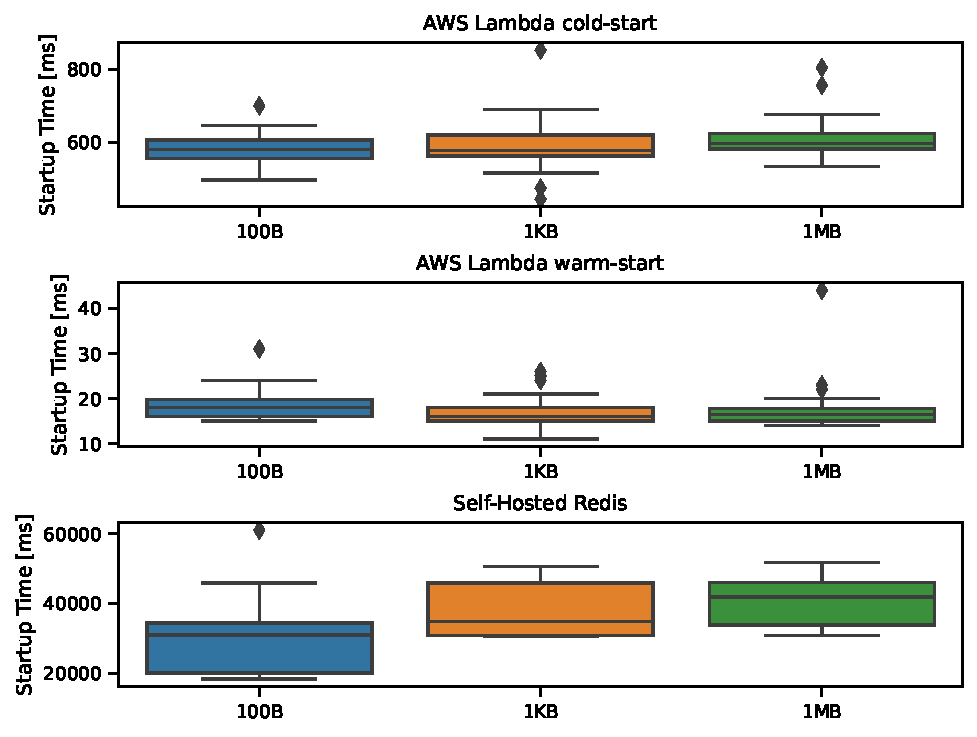
\includegraphics[width=0.8\textwidth]{figures/startup.pdf}
        \caption{Startup latency for the self-hosted Redis layer and the AWS Lambda function divided into cold and warm startups. Each experiment includes 30 measurements, and we also test different object sizes.}
        \label{fig:startup}
    \end{center}
\end{figure}

\chapter{Discussion}
\label{cha:discussion_and_outlook}
The evaluation yields some important insights into the performance of our system. Since our work serves as a proof-of-concept for building a reactive in-memory caching system with serverless computing, we have made some simplifications to make this possible within the scope of this work. Here we provide an overview of these limitations, while in the following sections, we elaborate on each limitation and suggest how our system can be extended to overcome them. We should note that the main reason for these limitations was the limited time for implementation. However, each section relates to the design goal of our system at the end and justifies the simplification. Finally, in Section~\ref{sec:usability} we summarize the discussion from the evaluation in terms of usability of our system. 

% Section~\ref{sec:limitations_and_restrictions} presents some limitations and constraints of our system that allowed us to build it as part of this work. In Section~\ref{sec:usability}, we summarize the discussion from the evaluation in terms of the usability of our system at the current state of implementation. The discussion highlights the usability of the serverless platform as a second in-memory caching layer to build a low-cost reactive in-memory caching system. Section~\ref{sec:outlook} explores how the limitations of our system can be overcome, and suggests future work to develop a fully managed in-memory caching system. 

% TODO: extend, why the limitation?, what was hard?, what was the reason? What would change and make it harder? 
\begin{itemize}
    \item Our system is currently only able to handle a single object (see Section ~\ref{sec:multiple_objects}).
    \item The scaling aspect is considered future work, as right now our system is based on a single AWS Lambda function with 1024 MB of memory and an EC2 instance of type \code{t2.micro} for the Redis layer, which limits the amount of data to be cached in our system (see Section~\ref{sec:scaling}).
    \item Consistency issues in our system are ignored for now by only supporting \code{get} requests (see Section~\ref{sec:api_extension}).
\end{itemize}

\section{Multiple Objects}
\label{sec:multiple_objects}
% one lambda function per object?
% https://aws.amazon.com/blogs/storage/turbocharge-amazon-s3-with-amazon-elasticache-for-redis/
% lazy loading as soon as Redis layer is running
% use multiple Redis instances if storage capacity reached
% For now, we only maintain a single connection to the running Lambda runtime, so as soon as the endpoint scheduler would invoke a second function to handle another object, the previously established connection would be lost. This behavior is not the result of a bug but rather due to the fact that we focused on other issues during this work. 
While the system is designed and mostly implemented to support multiple objects, proper connection management is missing. Supporting multiple objects raises some questions that we explore here in a theoretical framework that provides a foundation for potential future work. Our system can serve multiple objects within the same AWS Lambda function and self-hosted Redis instance, but how our endpoint scheduler works right now and how we handle connections prevents the system from adequately supporting multiple objects. While Redis is designed to cache multiple objects, using the serverless platform for multiple objects remains an open question. We think the best answer to this question is to use the endpoint scheduler as currently implemented on an object basis. So we call the Lambda function for a single object while the orchestrator and reverse proxy maintain multiple connections, with the key determining which connection leads to the Lambda runtime serving the desired object. Once the endpoint scheduler spins up the Redis instance, we apply the lazy loading technique and ignore the serverless platform. The orchestrator would need to keep track of the capacity of the Redis instance. If the capacity is exceeded, the serverless layer helps buffer the time required to set up the Redis cluster to expand its capacity. This has already opened the discussion on scaling, which will be continued in the next section.

~\\
Focusing on a single object already provides the opportunity to explore the possibilities of serverless computing for a reactive in-memory caching design. Covering multiple objects requires capacity management, which was not of central interest to us. Capacity management for Redis is not of much interest, as it only requires monitoring of running instances. The serverless platform includes one function per object and possibly splitting a large object into multiple functions, but this was already partially covered by InfiniCache~\cite{wang_infinicache_2020}.


% \begin{itemize}
%     \item Explain the limitations why our system does not support multiple objects.
%     \item Our system currently only relies on a single self-hosted Redis instance and the number of concurrent AWS Lambda connections is currently limited to 1.
%     \item So allowing multiple objects opens the question if our endpoint scheduler is acting on a per-object basis as of now, or if we keep the AWS Lambda layer for single objects, while as soon as we transition into the Redis state we forget about per-object processing.
%     \item Number of objects still restricted by the size of the single Redis instance. 
% \end{itemize}

\section{Scaling}
\label{sec:scaling}
% base cache system for the peak motivation
% about the peak motivation as discussed in the evaluation chapter
% discussion about potential required load balancer in fron of the reverse proxy
% multiple proxies requirement?
% Distributed Redis (Redis Cluster)
% Scalability:
% We don't want to reinvent a scalable in-memory cache such as Redis to deal with all the challenges in building a distributed in-memory storage. We focus on making in-memory capacity in a self-contained system available more quickly in case of burst workload. When we take a look at scaling, we can argue that we certainly have a base system running and our system woks to buffer unexpected load while our system relies on a Redis cluster. In this case we would have to think about the Redis part and whether we want to replace our fast spinning up empty Redis instance with an dynamically setup Read replica. This would result in a higher startup time of the Redis instance, which could be helped out by our Lambda layer on a per object base, while as soon as the Redis instance is running we no longer care about single objects workload but the whole workload in order to decide if the additional instance is no longer needed.
Our system attempts to use the serverless platform to improve a Redis-based in-memory caching system. The goal is not to develop an entirely new scalable in-memory cache, so our system is based on Redis as the core building block. While a Redis cluster theoretically provides scalability, the disadvantage of the ElastiCache managed service is the billing granularity based on node hours, resulting in poor cost efficiency when scaling is only required for short periods. Setting up the automation process for a self-hosted Redis cluster can lead to poor cost-efficiency or bad caching behavior for burst workloads. Scaling the Redis cluster relies on either ElastiCache or an automation process. Currently, our system only scales from zero to the size of one instance, focusing on burst workloads. Further scaling could be included in our system using our reactive design. So if we assume the scenario with a constant demand for in-memory caching (called base cache system), the more cost-effective solution would be to keep a Redis instance running to meet this demand constantly. Our system could form the basis to provide a managed scaling automation process for burst workloads on top of the constant demand. Our system could provide a lower-cost, fully managed service similar to ElastiCache by providing fine-grained elasticity through the reactive design of our system. There is still much work to be done to reach this level of implementation. However, the results of our system looked promising, so the direction described could help eliminate the need for an automation process and provide a cost-effective alternative to the AWS managed service.

% Our system could form the basis to provide a managed scaling automation process. We initially focused on the case of burst workloads while the in-memory caching system is not needed most of the time. We extend this scenario by assuming constant demand for in-memory caching. Compared to our system, the more cost-effective solution would be to keep a Redis instance running to meet this demand constantly. The scaling of the Redis cluster relies on either ElastiCache or an automation process. So assume our system includes a base cache system, a pure Redis base system, and uses the system developed as part of this work to handle unexpected short-term spikes. Our system could provide a lower-cost, fully managed service similar to ElastiCache by providing fine-grained elasticity through the reactive design of our system. There is still much work to be done to reach this level of implementation. However, the results of our system looked promising, so the direction described could help eliminate the need for an automation process and provide a cost-effective alternative to the AWS managed service.

~\\
By reducing the focus of our work on burst workloads, we can ignore the base cache system and focus more on the integration of the serverless platform in this particular setting. The base cache system is purely Redis-based and deals with the management of the self-hosted Redis cluster and its monitoring, which is not of central interest with respect to the serverless platform.

% \begin{itemize}
%     \item The previous discussion about multiple objects leads to the scaling issue on our system.
%     \item AWS Lambda can scale to infinity on a per-object basis, but what about the Redis layer?
%     \item Orchestrator can use a Redis Cluster to scale horizontally.
%     \item As soon as we enter this scale, we have to ask ourselves whether we are still in a scenario where our system actually makes sense.
%     \item Probably not, so instead we could assume that we have Redis Cluster running as a so-called base system and use our system on top of it to handle unexpected peaks which probably just include a few single objects. 
%     \item Explain the modification required to our system for this scenario on a high level.
%     \item Motivate this use case by taking the billing granularity of AWS ElastiCache into consideration, the comparison for self-hosted Redis is already provided in the evaluation.
% \end{itemize}

\section{Extension of the Reverse Proxy API}
\label{sec:api_extension}
% We’re building a cache for AWS S3, so we should care about what other S3 Actions (https://docs.aws.amazon.com/AmazonS3/latest/API/API_Operations.html) exists and if we integrate them to our system. For now we ignore the general S3 API and just provide a \code{get} endpoint to retrieve an object in our system. When someone uses the web interface to change an object, our caching system doesn’t know about it, especially the orchestrator, which tells the gateway that we have the specified object in the cache should be aware of it. We will not be able to integrate every action and some actions do not make sense in our case (e.g. delete bucket), but we should have an overview of the available actions and classify them. This way we can discuss classes of actions and justify why we ignore them or integrate them only partially.

% SET operations ()
% Support SET operations by creating a pipeline to update the cache as new data is written to S3. Using AWS Lambda function trigger, to keep the cache fresh as data is being written to S3, works for Redis layer, for Lambda layer, probably forcing the proxy to remove the forwarding would be best.
Our reverse proxy's API currently only supports \code{get} operations to retrieve objects specified by a key. Our reverse proxy stores information about keys when a particular in-memory layer is running, but we do not keep track of whether the object exists in S3, so requests for non-existing keys result in \emph{key not found}. This behavior is intentional, but it begs the question of what other S3 API operations are of interest to our system. If the client wants to push new objects, update existing objects, or delete existing objects, the S3 API should be used. In order to avoid retrieving a deleted object which was currently cached in our system, we have to consider those S3 API operations within the scope of our work. AWS Lambda function triggers would probably be the best way to accomplish this. Each time an object is added, updated, or deleted in the S3 bucket, a Lambda function is triggered to connect to our orchestrator to notify it of the event. If the object is not in the cache, our system does not care. However, suppose the object is in the cache and the client deletes or updates it. In that case, the orchestrator must either remove the cache entry and inform the reverse proxy or keep the cache up to date by retrieving the new object from persistent storage again. In both scenarios, the serverless layer would most likely require a manual shutdown of the function while the Redis layer could be updated dynamically. AWS Lambda function trigger is also the technique suggested by AWS when using ElastiCache to improve performance for S3 in combination with lazy loading~\cite{noauthor_turbocharge_2019}. So the only API endpoint our system would provide is the \code{get} endpoint, while the \code{put} and \code{delete} operations are supported via the S3 API, using AWS Lambda function triggers to keep our caching system up to date.

~\\
The issue of consistency is critical for building an in-memory caching system. However, in the context of this work exploring the possibilities of the serverless platform in a reactive system, it is sufficient to look at this aspect from a theoretical point of view.  


\section{Usability}
\label{sec:usability}
% small conclusion about the evaluation of our system and the actual usability of it
The applicability of our system in practice is currently limited by the restrictions mentioned in the previous section; as long as our system supports only one object, the applicability of our system is limited. Also, comparing our system with a fully managed service like ElastiCache, which supports auto-scaling, should be done with caution. 

~\\
However, for bursty workloads that inspired the reactive design of our system, using an additional in-memory layer based on serverless computing seems promising for building a cost-effective in-memory caching system. The current design of our reactive endpoint scheduler has issues with general workloads, where a pure Redis-based system is much more practical and cost-effective, but these issues will be addressed in future work. Interestingly, the fine-grained elasticity is limited in current managed services such as ElastiCache based on node hours. Therefore, we focused on burst workloads to address the elasticity issue for workloads that last less than an hour in this work.

~\\
The reactive design of our system aims to solve this very problem, where a simple automation process for self-hosted Redis would have difficulty provisioning the instance when in-memory caching is needed. We assume that developing an automation process capable of predicting future in-memory caching needs with a low error rate is rather infeasible, motivating the simple design of our reactive system. The reactive endpoint scheduler can provision in-memory caching using the serverless platform in less than a second. In the case of a warm startup, the serverless in-memory layer is even available within milliseconds. A pure Redis-based reactive system suffers from startup times of half a minute, so for workloads that last about a minute, our system significantly outperforms a pure Redis-based reactive system in terms of the in-memory portion served from the cache. Thus, serverless computing as an additional in-memory caching layer shows its potential in terms of the responsiveness of a reactive system. Building a cost-effective in-memory caching system using the less cost-effective serverless platform is counterintuitive. Therefore, our system can never beat a pure Redis-based reactive system in terms of cost. However, the improved responsiveness leads to a higher in-memory percentage, which is crucial for workloads lasting only a few minutes.

~\\
Suppose we can design a perfect automation process that is able to predict the arrival times of the workloads and thus run the self-hosted Redis instance for the exact duration of the workloads. This avoids any unnecessary over-provisioning, resulting in a perfect cost-efficient in-memory caching system. The feasibility of such a system is another matter. However, depending on the workload and its tail distribution, our system can achieve similar or even lower costs with an in-memory hit-rate of 95\%. 

~\\
Thus, the results of a Redis-based reactive in-memory caching system with serverless computing in this work look promising and provide a basis to improve the elasticity constraint on the node hours of current fully managed services without knowing the workload in advance.

% So, in summary, building a reactive Redis-based in-memory caching system with serverless computing looks promising for given situations, but the current state of the implementation clearly limits the use case of our system as a general in-memory caching service. Based on the foundation and design of our system, the outlook will show future work which targets to make our system more relevant and overcome any shortcoming to actually provide a scalable managed in-memory caching service similar to ElastiCache.

% However, if an application needs in-memory caching only in certain situations and for a short period of time, our system is able to beat a pure Redis-based system in terms of cost and still provide a high in-memory percentage. 


% \section{Outlook}
% \label{sec:outlook}
% % Consequences of your work?
% % Possible future work?
% In this section, we first address the limitations of our system and show how we can make our system more relevant as a managed in-memory caching service. The extension of our system described here shows the potential for building a scalable managed service similar to ElastiCache based on our work. The reactive design of our system helps minimize costs by avoiding over-provisioning in-memory caching resources. At the same time, the use of serverless computing mitigates the startup problem of a simple reactive automation process for a pure Redis-based system.

% \subsection{Limitations and Restrictions}
% This section refers to the issues mentioned in Section~\ref{sec:limitations_and_restrictions} and the necessary adjustments and considerations in our implementation to address them.

% \subsection{Improve Endpoint Scheduler}
% \label{sec:improve_endpoint_scheduler}
% The improvement of the endpoint scheduler offers many exciting starting points for future work. The reactive design of our endpoint scheduler could be improved by using proactive decisions. Integrating a proactive endpoint scheduler could help our system handle workloads where a reactive design leads to poor performance. However, integrating a proactive endpoint scheduler would require some prediction, which is not straightforward and opens a new research topic on its own. However, it would open many new possibilities for designing the endpoint scheduler.

% ~\\
% A more promising approach is offered by InfiniCache~\cite{wang_infinicache_2020} to provide caching for infrequent requests. Compared to our system, they do not use the serverless platform as a server listening to requests. Instead, their request directly invokes the function which stores the object. Using their system to manage the AWS Lambda execution environments to keep them warm allows for fast startup times and fast data retrieval. Extending our system by incorporating their approach to handling requests currently forwarded to S3 could improve average latency by achieving 100\% in-memory caching. The startup latencies measured in section~\ref{subsec:startup_times} look promising for warm lambda starts, and compared to these measurements, the reverse proxy would call the function itself, further reducing startup latency by eliminating the additional delay in message passing. Thus, integrating their approach could lead to a 100 percent in-memory caching system that can handle workloads that our system cannot respond to cost-efficiently. This adaption would also remove the direct impact of the system parameters concerning the in-memory portion.

% \subsection{Reverse Proxy as Client Library}
% \label{sec:proxy_as_client_library}
% Section~\ref{subsec:end_to_end_latency} has shown that the way we test and deploy our system is not ideal in the context of in-memory caching. Internet traffic latency accounts for a large portion of the end-to-end latency and drastically impacts the potential speedup. Deploying the reverse proxy on a separate EC2 instance requires an additional copy of the data, impacting end-to-end latency as object size increases. As long as the client/application runs outside the AWS infrastructure, we can only improve the simple copy. However, suppose the client/application is running in the AWS infrastructure. In that case, our reverse proxy could be wrapped in a client library that provides the same \code{get} API but runs on the same host as the application, similar to the design of InfiniCache~\cite{wang_infinicache_2020}. By customizing our system in this way, we can avoid the additional copy, resulting in better end-to-end latency for each layer, highlighting the latency difference between in-memory caching and the persistent storage layer. 

% The changes required are quite small as the reverse proxy has just to be wrapped inside a client library which is initialized at the beginning, while the communication with the orchestrator would remain the same. Further customization is required when multiple applications using the client library may be active at the same time. In this case, the orchestrator would need to manage multiple reverse proxy connections while the Lambda runtime connects to each running client library. These changes can be made relatively easily, but some additional adjustments are required when initializing a client library while our system is already up and running to keep the forwarding state consistent between all client libraries. 

% \subsection{Authentication and Security}
% \label{sec:authentication_and_security}
% % how do we check authentication for requests
% % what other security aspects are relevant or need to be considered
% \begin{itemize}
%     \item Authentication for requests?
%     \item What other security aspects are relevant or needed to be considered?
% \end{itemize}
\chapter{Related Work}
\label{cha:related_work}
This chapter gives a small insight into existing projects and research in related areas within the scope of this thesis. In Section~\ref{sec:in_memory_caching} we introduce the development of in-memory key-value stores such as Redis and newly proposed approaches. The various cloud services offer great opportunities to build multi-tier systems based on different services. We present examples of this approach in the area of cloud storage in Section~\ref{subsec:multi_layer_storage_system}. Since we use the serverless platform in our work as an additional in-memory layer, Section~\ref{sec:serverless_computing_rw} introduces work in the area of serverless computing and presents a system for caching large objects with serverless functions. In Section~\ref{sec:intermediate_data_caching}, we present a different view of caching than latency improvement.

\section{In-Memory Caching}
\label{sec:in_memory_caching}
In-memory caching will continue to be a hot topic in research and academia due to the increasing amount of data in daily applications and the desire for the best possible performance. Redis and Memcached are two popular and well-known in-memory caching solutions supported by cloud providers through managed services such as ElastiCache~\cite{noauthor_amazon_nodate-1}, Google Memorystore~\cite{noauthor_memorystore_nodate}, and Azure Cache~\cite{noauthor_azure_nodate}. 

~\\
While most modern applications rely on such a managed service to improve performance in some way, Facebook has even developed its own distributed key-value store to meet its specific needs based on Memcached~\cite{nishtala_scaling_nodate}. These managed in-memory caching services are commonly used to accelerate the performance of a persistence storage service. In the context of our work, we focused on S3 and Redis with ElastiCache as the managed service. The same principle is found in other services such as AWS DynamoDB~\cite{noauthor_fast_nodate}, a fully managed NoSQL database service. DynamoDB Accelerator (DAX) is a fully managed caching service to increase performance for read-intensive workloads~\cite{noauthor_amazon_2017}.

~\\
There are numerous case studies and analyses on existing in-memory key-value stores~\cite{kaur_-memory_2018, chen_towards_2016, lubis_multi-thread_2015} and their workload~\cite{atikoglu_workload_2012}. With the changing requirements and limitations of existing systems, they are constantly evolving, or even new systems are proposed to overcome these problems. Thus, improvements to Redis such as memory management optimization~\cite{zhang_redis_2018} and multi-thread support~\cite{lubis_multi-thread_2015} are not uncommon. Other systems such as MICA focus on multicore architectures to improve performance for write-intensive workloads~\cite{lim_mica_2014}. BlueCache uses flash memory and a flash controller implemented directly in hardware to achieve comparable performance at a lower memory cost by avoiding DRAM~\cite{xu_bluecache_2016}. Mega-KV's proposed use of GPUs to improve performance~\cite{zhang_mega-kv_2015}. Bullet attempts to combine the advantages of byte-addressable persistent memory with the lower latency of DRAM to build a key-value store~\cite{huang_closing_2018}. Or Minos, which uses size-aware sharding to improve performance~\cite{didona_size-aware_2018}.

% paragraph about serverless computing and the work done in this are (some connection to in-memory storage possible?)
\section{Multi-Layer Storage Systems}
\label{subsec:multi_layer_storage_system}
Different storage systems offer a specific trade-off between cost, latency, and capacity. So while S3 offers higher latency with lower cost and unlimited capacity, ElastiCache offers much lower latency with limited capacity and higher cost. In our work, we do not try to reinvent an existing storage system but rather combine the advantageous features of some systems to create an overall better system. An example in this direction is Anna~\cite{wu_autoscaling_2019}. This efficient key-value store can scale not only horizontally but also vertically with respect to different storage levels and thus different cost/performance ratios. Vertical scaling thus includes an in-memory tier using the memory of EC2 instances, a flash storage tier using Elastic Block Store (EBS), and possibly other tiers such as S3 and even S3 Glacier\footnote{AWS S3 Glacier is a low-cost archive storage.}. The system automatically adapts to the monitored workload using a reactive policy engine. The policy engine attempts to derive the most cost-effective policies according to the objective set by the system administrator.

\section{Serverless Computing}
\label{sec:serverless_computing_rw}
Systems such as Cloudburst~\cite{sreekanti_cloudburst_2020}, which uses Anna under the hood, or Pocket~\cite{klimovic_pocket_nodate} are proposed as solutions for the serverless platform to enable stateful functions and cost-effective data sharing. InfiniCache~\cite{wang_infinicache_2020}, on the other hand, uses the serverless platform to build a cost-effective object caching system. Their system uses the memory resources of AWS Lambda's execution environments to store objects and only pays for the resources once the function is actually executed. By cleverly orchestrating their functions and maintaining their execution environment with so-called warm-up operations, they have built a pay-per-use caching system based on requests rather than node hours, as is the case with popular in-memory caching services like ElastiCache.

\section{Intermediate Data Caching}
\label{sec:intermediate_data_caching}
Another interesting use case is CPU-bound applications, where many resources are consumed to repeatedly compute values, while in-memory caching allows these values to be computed only once. An interesting paper on this topic evaluates the trade-off between recomputing data items or caching them in a cloud storage service such as S3~\cite{scouarnec_cache_2014}. Their system uses an analytical model with the assumption of a specific distribution for request arrival times. The right cache policies can be derived in terms of cost, reducing the cost of a cloud-based system.

% InfiniCache: Exploiting Ephemeral Serverless Functions to Build a Cost-Effective Memory Cache~\cite{wang_infinicache_2020}.
% Autoscaling Tiered Cloud Storage in Anna~\cite{wu_autoscaling_2019}.
% Cloudburst: Stateful Functions-as-a-Service~\cite{sreekanti_cloudburst_2020}.
% Pocket: Elastic Ephemeral Storage for Serverless Analytics~\cite{klimovic_pocket_nodate}.
% AutoSight: Distributed Edge Caching in Short Video Network~\cite{zhang_autosight_2020}.
% DeepCache: A Deep Learning Based Framework For Content Caching~\cite{narayanan_deepcache_2018}.
% Cache policies for cloud-based systems: To keep or not to keep~\cite{scouarnec_cache_2014}.
% Shuffling, Fast and Slow: Scalable Analytics on Serverless Infrastructure~\cite{pu_shuffling_2019}.
% Scaling Memcache at Facebook~\cite{nishtala_scaling_nodate}.
\chapter{Conclusion and Outlook}
\label{cha:conclusion_and_outlook}
% Final, short summary of your work.
In this work, we explore the applicability of the serverless platform as an additional in-memory caching layer. We propose a novel reactive in-memory caching system that relies on the primary Redis-based caching layer, similar to other managed cloud services like ElastiCache. By leveraging the memory capacity of serverless functions, our system can improve the responsiveness of a reactive design without over-provisioning in-memory caching resources. Compared to the billing granularity of node hours of current managed in-memory caching services, our system can provide fine-grained control and therefore provides better elasticity to build a cost-effective in-memory caching system. The reactive design forms the basis for a fully managed service that frees system administrators from the burden of managing the in-memory cache themselves in a cost-effective manner, depending on the workload.

~\\
The main contribution of our work is the reactive design of our orchestrator, which is responsible for managing the in-memory caching layers and the integration of the serverless platform as one of these layers. Our system is deployed on AWS infrastructure and uses EC2 units to host our Redis-based layer, while AWS Lambda is the serverless platform used in our system. The reactive design enables our orchestrator to manage the in-memory caching layers without over-provisioning caching resources cost-effectively. Our orchestrator can provision in-memory caching capacity within milliseconds using the serverless platform. Afterward, the system switches to the less expensive Redis-based layer when the load persists. However, starting the Redis layer takes some time; the intermediate time can also be covered with the serverless platform.

~\\
Cost efficiency and performance guarantees are highly dependent on the workload, as the reactive design acts based on this load. Simulations are used to evaluate and study the usability and cost of our system for different workloads. The current design of our system clearly shows some limitations for general workloads, as the reactive mechanism is designed to handle burst workloads. We target this setting because the current managed services are not cost-effective due to their design, while a self-managed system is challenging to develop for the unknown arrival of these burst workloads. The results show that our reactive system achieves a cache hit rate of about 95\% in this setting. In the case of bursty workloads, our system can reduce the cost of an always running caching system and achieves similar or even lower costs than a self-hosted Redis instance running only for the duration of the workload. The evaluation clearly shows the potential of our reactive design and serverless computing in such a system. 

\newpage
\noindent
Although our work targets whether the serverless platform is useful for building a reactive managed system, the implementation still requires future work to overcome current limitations. In addition, we propose some interesting directions for future work:
\begin{itemize}
    \item \textbf{Proactive Endpoint Scheduler:} Incorporating a proactive endpoint scheduler could help our system handle workloads where a reactive design leads to poor performance. A proactive endpoint scheduler would require prediction, a separate research topic.
    \item \textbf{InfiniCache:} InfiniCache~\cite{wang_infinicache_2020} provides a novel approach to in-memory caching as a request-based pay-per-use model. Integrating their approach for infrequent requests could help our system become a 100\% in-memory caching system.
    \item \textbf{Client Library:} Suppose the client is running inside the AWS infrastructure. The additional copy on the reverse proxy can be avoided by including the reverse proxy in a client library running on the same host as the client, similar to InfiniCache~\cite{wang_infinicache_2020}.
\end{itemize}

% Our work provides a solid foundation for future work on extending our system to compete with a managed cloud service such as ElastiCache. Our work builds a solid foundation for future work to extend our system to compete with a managed cloud service like ElastiCache.

% \section{Improve Endpoint Scheduler}
% \label{sec:improve_endpoint_scheduler}
% The improvement of the endpoint scheduler offers many exciting starting points for future work. The reactive design of our endpoint scheduler could be improved by using proactive decisions. Integrating a proactive endpoint scheduler could help our system handle workloads where a reactive design leads to poor performance. However, integrating a proactive endpoint scheduler would require some prediction, which is not straightforward and opens a new research topic on its own. However, it would open many new possibilities for designing the endpoint scheduler.

% ~\\
% A more promising approach is offered by InfiniCache~\cite{wang_infinicache_2020} to provide caching for infrequent requests. Compared to our system, they do not use the serverless platform as a server listening to requests. Instead, their request directly invokes the function which stores the object. Using their system to manage the AWS Lambda execution environments to keep them warm allows for fast startup times and fast data retrieval. Extending our system by incorporating their approach to handling requests currently forwarded to S3 could improve average latency by achieving 100\% in-memory caching. The startup latencies measured in Section~\ref{subsec:startup_times} look promising for warm Lambda starts, and compared to these measurements, the reverse proxy would call the function itself, further reducing startup latency by eliminating the additional delay in message passing. Thus, integrating their approach could lead to a 100 percent in-memory caching system that can handle workloads that our system cannot respond to cost-efficiently. This adaption would also remove the direct impact of the system parameters concerning the in-memory portion.

% \section{Reverse Proxy as Client Library}
% \label{sec:proxy_as_client_library}
% Section~\ref{subsec:end_to_end_latency} has shown that the way we test and deploy our system is not ideal in the context of in-memory caching. Internet traffic latency accounts for a large portion of the end-to-end latency and drastically impacts the potential speedup. Deploying the reverse proxy on a separate EC2 instance requires an additional copy of the data, impacting end-to-end latency as object size increases. As long as the client runs outside the AWS infrastructure, we can only improve the simple copy. However, suppose the client is running on the AWS infrastructure. In that case, our reverse proxy could be wrapped in a client library that provides the same \code{get} API but runs on the same host as the client, similar to the design of InfiniCache~\cite{wang_infinicache_2020}. By customizing our system in this way, we can avoid the additional copy, resulting in better end-to-end latency for each layer, highlighting the latency difference between in-memory caching and the persistent storage layer. 

\clearpage

\addcontentsline{toc}{chapter}{References}
% \bibliographystyle{acm}
\bibliographystyle{IEEEtran}
\bibliography{IEEEabrv, zotero}

\clearpage
\appendix
\pagenumbering{Roman}

\chapter{Appendix}
\label{app:a}
% - material which is not absolutely necessary to understand and follow the work
% - code snippets
% - additional plots

\section{AWS Setup}
\label{sec:aws_setup}
% include relevant details for the setup on the AWS platform
% setup of the building blocks in general
% network specific configurations (VPC, inbound rules)
In Appendix~\ref{subsec:deployment} we describe how our system can be used and what to consider regarding the AWS infrastructure on which our system runs. First, we explain how the orchestrator and Reverse Proxy instances obtain their executable binaries, while Appendix~\ref{subsec:network_configuration} provides some details on the network configurations required for the necessary communication, followed by some clarifications on the security concerns in the context of this work and implementation in Appendix~\ref{subsec:security_concerns}. In Appendix~\ref{subsec:self_hosted_redis_instance} we describe the instance that hosts the Redis server.

\subsection{Deployment}
\label{subsec:deployment}
While our system dynamically determines the IP addresses used for communication, the instance ID for the orchestrator is fixed in the source code so that the reverse proxy can establish initial communication at startup. We have also set the instance ID for the self-hosted Redis instance, since we are focusing on a single instance for the purposes of this work. The scripts \code{build\_gateway.sh} and \code{build\_orchestrator.sh} can be used to create the executable binaries for the reverse proxy and orchestrator. The script allows you to specify the IP address of the instance that hosts it to transfer the executable to the corresponding instance. The \code{build\_lambda.sh} script creates the executable file for the Lambda layer and updates the function code of the existing Lambda function. Starting the system requires executing the orchestrator binary, followed by the reverse proxy binary.

\subsection{Network Configuration}
\label{subsec:network_configuration}
In order to execute/transfer the binaries, the EC2 instances must allow incoming traffic to enable SSH access. We briefly cover the AWS infrastructure settings related to VPCs and security groups. Everything we deploy is within our standard VPC provided by AWS. The associated security group for each EC2 instance contains rules to allow inbound network traffic for the required ports used for communication. In addition, we allow incoming traffic for port 22 for SSH communication. The way our system performs connection management for the Lambda layer requires a special inbound rule for our orchestrator and reverse proxy. The port used to listen to communication from the Lambda runtime must restrict the source to the VPC. Therefore, the Lambda function must be configured within the same VPC, which is the case as long as we only use the default VPC.

\subsection{Security Concerns}
\label{subsec:security_concerns}
Security was outside the scope of this work, so we could ignore most of the AWS-specific settings. Some exceptions, such as the network configuration mentioned above, and some specific settings are briefly discussed in this section. The session required by the \code{aws-sdk-go} used for various parts of our work is obtained from environment variables that contain the required information for the AWS account. The Lambda function is configured with a specific execution role for permission to access the S3 bucket.

\subsection{Self-Hosted Redis Instance}
\label{subsec:self_hosted_redis_instance}
This section covers the EC2 instance hosting a Redis server for our in-memory caching layer. The instance itself does not restrict incoming traffic, while access management is performed by the Redis server itself and requires a password. The password is hard coded in the source code, as it is required by both the orchestrator and the reverse proxy. The Redis server on this instance is set up to run as daemon as soon as the instance is started~\cite{hsieh_spin_2020}.

\section{System Configurator Algorithm}
\label{sec:system_configurator_algorithm}
Our current system configurator is a simple step function, as it only helped us explore the impact of system parameters on our simulations. While experimenting with lower rate workloads, we found that our system needs some sort of information about the average rate of incoming requests in order to set appropriate parameters for our endpoint scheduler. Therefore, the first input parameter for our system configurator is the rate parameter, which describes the average number of requests per minute. The second parameter describes the sensitivity value, which we have already described. The pseudocode below shows the step function algorithm for deriving the system parameters according to the input:
\begin{algorithm}
    \caption{System Configurator}\label{alg:system_configurator}
    \begin{algorithmic}
        \Procedure{GetSystemParamaeters}{rate, sensitivity}
            \State $maxSens \gets 5$
            \State $lambdaWindowElements \gets 2$
            \State $redisThreshold \gets 4$

            \State $t \gets 60.0/rate$ \Comment{Seconds between two requests on average}
            \State $tick \gets (t - ((maxSens - sensitivity) \times (t / maxSens)))$ \Comment{Duration in seconds}
            \State $lambdaThreshold \gets (tick \times lambdaWindowElements)$ \Comment{Duration in seconds}
            \State $redisUtilization \gets (t \times (sensitivity+5))$ \Comment{Duration in seconds}
            \State \Return system parameters
        \EndProcedure
    \end{algorithmic}
\end{algorithm}

\newpage
\begin{landscape}
    \section{Simulation Overview}
    \label{sec:simulation_overview}
    \begin{table*}[ht!]
        \centering
        \ra{1.2}
        \begin{adjustbox}{max width=\linewidth}
        \begin{tabular}{ @{} l r r r r r c r r r c r r c r @{}}
        \toprule
        & \multicolumn{5}{c}{\textbf{AWS Lambda}} & \phantom{abc} & \multicolumn{3}{c}{\textbf{Self-Hosted Redis}} & \phantom{abc} & \multicolumn{2}{c}{\textbf{AWS S3}} & \phantom{abc} & \phantom{abc} \\
        \cmidrule{2-6} \cmidrule{8-10} \cmidrule{12-13}
        \textbf{Simulation} & \textbf{Duration} & \textbf{Cost} & \textbf{Inv.} & \textbf{Cold} & \textbf{Cost} && \textbf{Duration} & \textbf{Inv.} & \textbf{Cost} && \textbf{Req.} & \textbf{Cost} && \textbf{Total Cost}\\
        \midrule
        Figure~\ref{fig:ec2log_3_2} &   556170ms & 0.00929 & 36 & 3 & 0.0000072 && 1020s & 1 & 0.00377 && 81  & 0.0000348 && 0.0131 \\
        Figure~\ref{fig:ec2log_3_3} &   393809ms & 0.00657 & 10 & 4 & 0.0000020 && 2040s & 2 & 0.00759 && 31  & 0.0000133 && 0.0142 \\
        Figure~\ref{fig:ec2log_3_4} &   161806ms & 0.00270 & 4 &  1 & 0.0000008 && 2701s & 1 & 0.01005 && 13  & 0.0000056 && 0.0128 \\
        Figure~\ref{fig:ec2log_s3} &    x &        x &       x &  x & x         && x     & x & x       && 175 & 0.0000753 && 0.0000753 \\
        Figure~\ref{fig:ec2log_ec} &    x &        x &       x &  x & x         && x     & x & x       && 1   & 0.00000043 && 0.019 \\
        Figure~\ref{fig:poisson_3_2} &  328207ms & 0.00548 & 27 & 1 & 0.0000054 && 0s    & 0 & 0       && 69  & 0.0000296 && 0.00552 \\
        Figure~\ref{fig:poisson_3_3} &  499976ms & 0.00835 & 21 & 1 & 0.0000042 && 281s  & 1 & 0.00105 && 46  & 0.0000198 && 0.00942 \\
        Figure~\ref{fig:poisson_3_4} &  381188ms & 0.00637 & 10 & 2 & 0.0000020 && 859s  & 2 & 0.00320 && 26  & 0.0000112 && 0.00958 \\
        Figure~\ref{fig:poisson_3_5} &  506881ms & 0.00846 & 11 & 1 & 0.0000022 && 849s  & 2 & 0.00316 && 23  & 0.0000099 && 0.0116 \\
        Figure~\ref{fig:poisson_4_2} &  350962ms & 0.00586 & 31 & 1 & 0.0000062 && 300s  & 1 & 0.00112 && 76  & 0.0000327 && 0.00702 \\
        Figure~\ref{fig:poisson_4_3} &  512991ms & 0.00857 & 31 & 1 & 0.0000062 && 437s  & 1 & 0.00163 && 62  & 0.0000267 && 0.0102 \\
        Figure~\ref{fig:poisson_4_4} &  817102ms & 0.01365 & 17 & 1 & 0.0000034 && 681s  & 4 & 0.00253 && 35  & 0.0000151 && 0.0162 \\
        Figure~\ref{fig:poisson_4_5} &  266881ms & 0.00446 & 3 &  1 & 0.0000006 && 1500s & 2 & 0.00558 && 8   & 0.0000034 && 0.0100 \\
        Figure~\ref{fig:spike_1} &      61531ms &  0.00103 & 5 &  1 & 0.0000010 && 240s  & 1 & 0.00089 && 9   & 0.0000039 && 0.00193 \\
        Figure~\ref{fig:spike_2} &      51477ms &  0.00086 & 3 &  1 & 0.0000006 && 421s  & 1 & 0.00156 && 12  & 0.0000052 && 0.00243 \\
        Figure~\ref{fig:spike_3} &      76754ms &  0.00128 & 7 &  1 & 0.0000014 && 601s  & 1 & 0.00224 && 16  & 0.0000069 && 0.00353 \\
        Figure~\ref{fig:spike_4} &      129234ms & 0.00216 & 10 & 1 & 0.0000020 && 1141s & 1 & 0.00425 && 31  & 0.0000133 && 0.00642 \\
        \bottomrule
        \end{tabular}
        \end{adjustbox}
        \caption{More detailed insights for each layer during our simulation. Parameters were either logged by the orchestrator or queried by AWS CloudWatch. Total costs are derived from these observations. Costs are in USD for the Europe (Frankfurt) region and are calculated according to the base costs of the specified units (EC2, ElastiCache, Lambda). The table contains the total billed time for Lambda and the cost. The total number of function calls, the number of cold starts, and the cost in terms of function invocations. For the self-hosted Redis tier, we show the total billed duration (the minimum billed duration of 60 seconds is already included), the number of starts, and the cost in terms of duration. S3 includes the total number of requests, including the cold-starts and Redis starts and the associated cost. The last column shows the total cost for the simulation.}
        \label{tab:costs}
    \end{table*}
\end{landscape}

\section{Offline Endpoint Scheduler Algorithm}
\label{sec:offline_endpoint_scheduler_algorithm}
% TODO: short explanation and reference to actual code
The offline endpoint scheduler allows us to evaluate the performance of our endpoint scheduler by presenting an algorithm with complete information about the incoming workload. The algorithm derives a cost-effective use of our in-memory caching layer with respect to the assumptions and calculations presented in Section~\ref{sec:offline_endpoint_scheduler}. The core logic of the algorithm is presented in the same section, while the following pseudocode provides a more detailed description.

\algnewcommand\algorithmicswitch{\textbf{switch}}
\algnewcommand\algorithmiccase{\textbf{case}}
\algnewcommand\algorithmicassert{\texttt{assert}}
\algnewcommand\Assert[1]{\State \algorithmicassert(#1)}%
% New "environments"
\algdef{SE}[SWITCH]{Switch}{EndSwitch}[1]{\algorithmicswitch\ #1\ \algorithmicdo}{\algorithmicend\ \algorithmicswitch}%
\algdef{SE}[CASE]{Case}{EndCase}[1]{\algorithmiccase\ #1}{\algorithmicend\ \algorithmiccase}%
\algtext*{EndSwitch}%
\algtext*{EndCase}%

\begin{algorithm}[H]
    \caption{Checks if next request should be served by individual Lambda runtime.}\label{alg:offline_endpoint_scheduler2}
    \small
    \begin{algorithmic}
        \Procedure{checkStart}{}
            \If{next 9 requests within $90$ seconds}
                \State $lambdaList \gets$ append $30s$ Lambda runtime
                \State $redisList \gets$ append $60s$ Redis runtime
                \State $state \gets redis$
            \Else
                \State $lambdaList \gets$ append $5s$ Lambda runtime
                \State $state \gets lambda$
            \EndIf
        \EndProcedure
    \end{algorithmic}
\end{algorithm}
\begin{algorithm}[H]
    \caption{Offline Endpoint Scheduler}\label{alg:offline_endpoint_scheduler}
    \small
    \begin{algorithmic}
        \State $state \gets none$
        \State $lambdaList, redisList \gets$ empty list \Comment{Keep track of Lambda start and end times}
        \While{further requests to process}
        \Switch{$state$}
            \Case{$none$}
                \State \Call{checkStart}{}
            \EndCase
            \Case{$lambda$}
                \If{Lambda runtime still running}
                    \If{next 9 requests within $90$ seconds}
                        \State $lambdaList \gets$ extend last runtime by $30s$
                        \State $redisList \gets$ append $60s$ Redis runtime
                        \State $state \gets redis$
                    \Else
                        \State $lambdaList \gets$ extend last runtime by $5s$
                    \EndIf
                \Else
                    \State \Call{checkStart}{} \Comment{Lambda runtime not running}
                \EndIf
            \EndCase
            \Case{$redis$}
                \If{Redis still running}
                    \State continue
                \ElsIf{next request withing $104.6$ seconds} \Comment{Redis not running}
                    \State extend Redis runtime
                \Else
                    \State \Call{checkStart}{}
                \EndIf
            \EndCase
        \EndSwitch
        \EndWhile
    \end{algorithmic}
\end{algorithm}

\end{document}
